%% UTFPRCT-TEX, v1.0.6 wmeira on 2021/10/11
%% Copyright (C) 2020- by William H. T. Meira
%%
%% Modified version of project 'utfprpgtex' maintained 
%% by Luiz E. M. Lima
%%
%% This work may be distributed and/or modified under the
%% conditions of the LaTeX Project Public License, either version 1.3
%% of this license or (at your option) any later version.
%% The latest version of this license is in 
%%   http://www.latex-project.org/lppl.txt
%% and version 1.3 or later is part of all distributions of LaTeX
%% version 2005/12/01 or later.
%%
%% This work has the LPPL maintenance status `maintained'.
%%
%% The Current Maintainer of this work is William H. T. Meira.
%%
%% This project consists mainly of files: 'utfprct.cls', 'utfprct.tex', 
%% 'utfprct-dados.tex' 
%% 
%% The 'abntex2-alf.bst' and 'abntex2-num.bst' files are slightly
%% modified versions of the bibtex styles from abntex2 (v.1.9.7)
%% package to suit NBR6023/2018 (not yet implemented there). 
%% Complementary, 'abntex2-alf-en.bst' and 'abntex2-num-en.bst' are
%% english versions of the respective bibtex styles.
%%
%% Contribute to improve this project (github repo):
%% https://github.com/wmeira/utfprct-tex

%% Formato digital (sem folhas em branco): 
%% 'pretextualoneside': impressão dos elementos pré-textuais começa em qualquer lado da folha (anverso ou verso)
%% 'oneside': impressão dos elementos textuais e pós-textuais no anverso da folha (sem folhas em branco para o verso)

%% Formato impresso:
%% 'pretextualtwoside': impressão dos elementos pré-textuais começa sempre no anverso
%% 'oneside' ou 'twoside': impressão dos elementos textuais e pós-textuais `oneside` (anverso) ou `twoside` (anverso e verso, se mais de 100 páginas)

%% [Note] As legendas devem ser colocadas em cima do elemento (figura, tabela, quadro, algoritmo...) e os  \caption antes de entrar no ambiente. Obrigatoriamente, \fonte deve ser embaixo da elemento. Se for de criação do próprio autor, colocar "Autoria Própria." (Own Authorship.)
%\begin{figure}[htb]%% Ambiente figure
%\caption{Exemplo de caption}%% Legenda
%\label{fig:figura1}%% Rótulo
%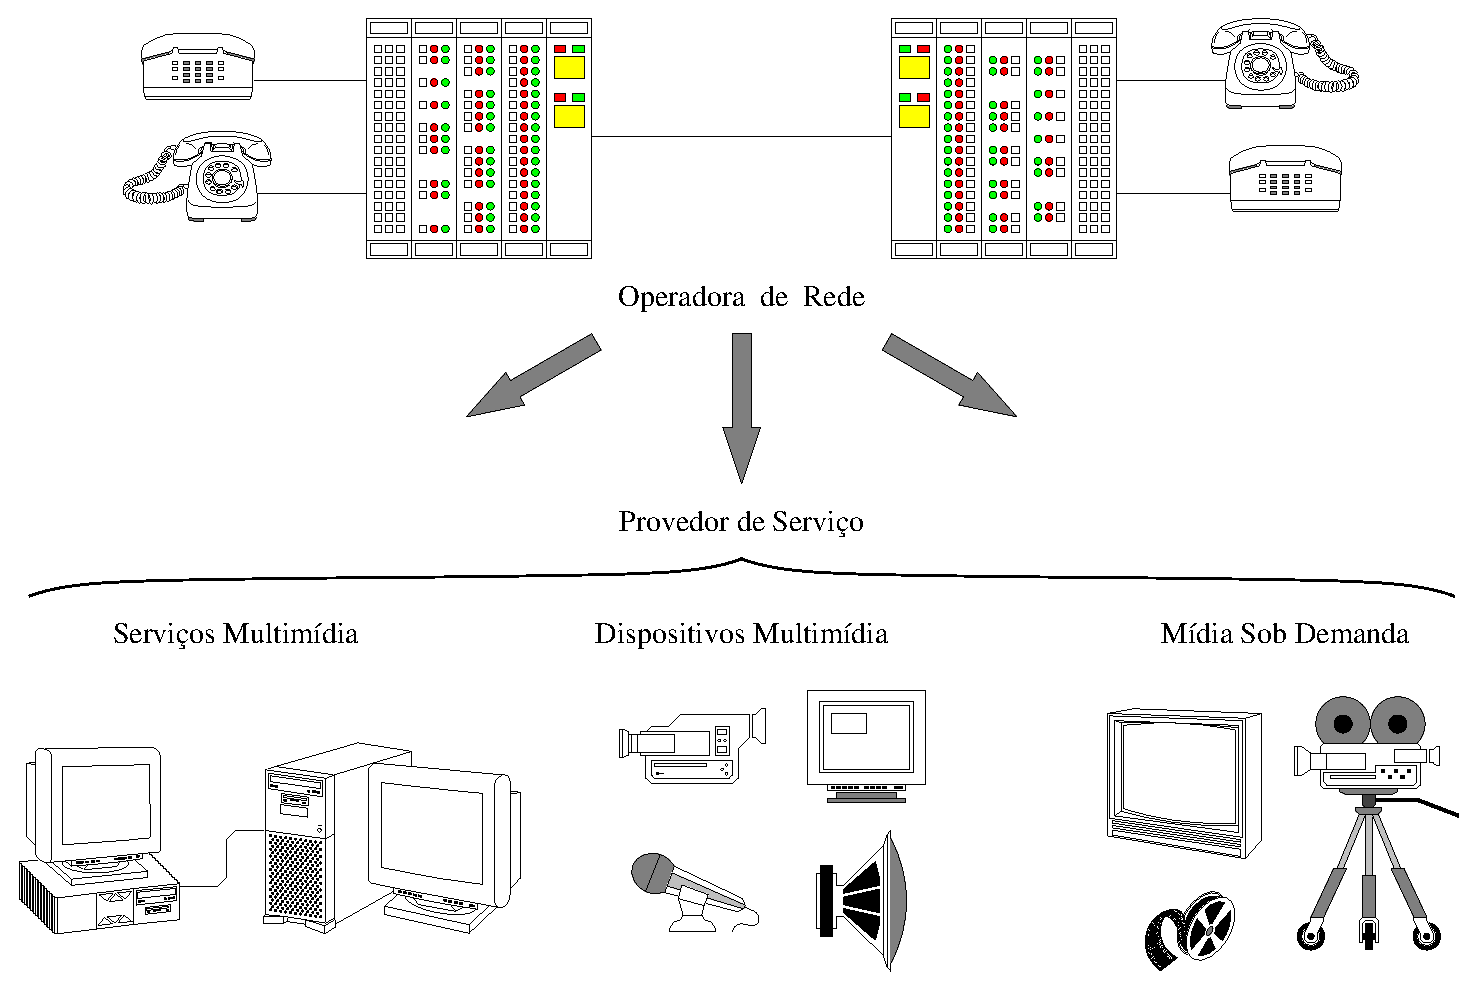
\includegraphics[width=\textwidth]{./CapituloExemplo/figura1}%% Dimensões e localização
%\fonte{\citet{Larsson2003}.}%% Fonte (quando criado pelo autor, usar Autoria Própria)
%\end{figure}

%% Classe e opções de documento
\documentclass[%% Opções
%% -- Opções da classe MEMOIR --
  12pt,%% Tamanho da fonte: 10pt, 11pt, 12pt, etc.
  a4paper,%% Tamanho do papel: a4paper (A4), letterpaper (carta), etc.
  % fleqn,%% Alinhamento das equações à esquerda (comente para alinhamento centralizado)
  % leqno,%% Numeração das equações no lado esquerdo (comente para lado direito)
  oneside,%% IMPRESSÃO dos elementos textuais e pós-textuais: oneside (apenas no anverso) ou twoside (anverso e verso, se mais de 100 p.) (insere páginas em branco).
%%  
%% -- Opções da classe ABNTEX2 --
  sumario = abnt-6027-2012,%% Formatação do sumário: tradicional (estilo tradicional) ou abnt-6027-2012 (norma ABNT 6027-2012)
  chapter = TITLE,%% Títulos de capítulos em maiúsculas (comente para desabilitar)
  section = TITLE,%% Títulos de seções secundárias em maiúsculas (comente para desabilitar)
  % subsection = TITLE,%% Títulos de seções terciárias em maiúsculas (comente para desabilitar)
  % subsubsection = TITLE,%% Títulos de seções quartenárias em maiúsculas (comente para desabilitar)
%%  
%% -- Opções da classe UTFPRCT-TEX --
  pretextualoneside,%% Impressão dos elementos pré-textuais: pretextualoneside (anverso) ou pretextualtwoside (anverso e verso)
  fontetimes,%% Fonte do texto: fontetimes (times), fontearial (arial) ou fontecourier (courier), fontemodern (lmodern - default latex). Times and Arial are ABNT recommended
   %vinculoscoloridos,%% Cores nos vínculos (citações, arquivos, links, url, etc.) (comente para desabilitar). NBR 14724/2011: cor preta (inclusive hyperlinks)
  semrecuonosumario,%% Remoção do recuo dos itens no sumário (comente para adição do recuo, se estilo tradicional)
  %inserirbackref,%% Inserir backref na lista de referências (e.g., Citado na página...)
  usemakeindex,%% Compilação de glossários e índices utilizando makeindex (comente para desabilitar)
  legendascentralizadas,%% Alinhamento das legendas centralizado (comente para alinhamento à esquerda)
%%  
%% -- Opções da folha de aprovação -- 
%% O mais comum é anexar o PDF do termo de aprovação sem assinaturas. As opções abaixo são para o formato da pós-graduação UTFPR-PG (Ponta Grossa) e podem servir de placeholder para este template.
  %aprovacaoestiloppg,%% Folha de aprovação do programa de pós-graduação no estilo do PPG (comente para estilo padrão)
  %pardeassinaturas,%% Assinaturas na folha de aprovação em até duas colunas (comente para em uma única coluna)
  % linhasdeassinaturas,%% Linhas de assinaturas na folha de aprovação (comente para remover as linhas)
%%  
%% -- Opções do pacote babel (hifenização) -- % 
  %french,%% Idioma adicional para hifenização (suporte parcial)
  %spanish,%% Idioma adicional para hifenização (suporte parcial)
  english,%% Idioma adicional para hifenização  (colocar em último para doc. em inglês)  
  brazil%% Idioma principal do documento (último da lista) 
]{utfprct}%% Classe utfprct

%%%%%%%%
% Documento em Inglês: colocar o "english" como último idioma carregado no documentclass, sendo o último a língua principal do documento.
%%%%%%%%

%%%%%%%%
%% Configuração dos avisos (warnings)
%% Comportamento do Tex quando um PDF é incluído e possui uma versão mais nova que a versão mínima especificada em \pdfminorversion. Opções: -1 (no info), 0 (default, warning), 1 (error)
\pdfinclusionerrorlevel=-1%no warning 
%\pdfminorversion=5%pdf minor output version (default 5)

%% [Badbox] Underfull e Overfull nível de aviso (filtra o que está abaixo)
\hbadness=5000%0 até 10000 (max) nível de badness
\vbadness=1000%0 até 10000 (max) nível de badness
%\hfuzz=0.01pt%excesso permitido de largura (\hbox)para ser considerado overfull
%\vfuzz=0.001pt%excesso permitido de altura (\vbox) para ser considerado overfull
%\overfullrule=10mm%adicionar aviso visual para um badbox
%%%%%%%%

%%%%%%%%
%% Pacotes carregados nas classes:
%%   memoir: abstract, appendix, array, booktabs, ccaption, chngcntr, chngpage, dcolumn, delarray, enumerate, epigraph, framed, ifmtarg, ifpdf, index, makeidx, moreverb, needspace, newfile, nextpage, parskip, patchcmd, setspace, shortvrb, showidx, tabularx, titleref, titling, tocbibind, tocloft, verbatim, verse.
%%   memoir (similares): crop, fancyhdr, geometry, sidecap, subfigure, titlesec.
%%   abntex2: babel, bookmark, calc, enumitem, ifthen, hyperref, textcase.
%%   utfprct: abntex2cite, ae, algorithmic, amsmath, backref, breakurl, caption, subcaption, cmap, color, eepic, epic, epsfig, etoolbox, fancyhdr, fix-cm, fontenc, glossaries, graphics, graphicx, helvet, hyphenat, indentfirst, inputenc, lastpage, morewrites, nomencl, sfmath, sistyle, substr, times, xtab, pdfpages.

%% Pacotes adicionais (\usepackage[options]{package})
\usepackage{bigdelim, booktabs, colortbl, longtable, multirow}%% Ferramentas para tabelas
\usepackage{amssymb, amstext, amsthm, icomma}%% Ferramentas para linguagem matemática
\usepackage{pifont, textcomp, wasysym}%% Símbolos de texto

% Refinamento tipográfico: diminui badboxes
\usepackage{microtype}%

%% Comandos personalizados (\newcommand{name}[num]{definition})
\newcommand{\cpp}{\texttt{C$++$}}%% C++
\newcommand{\latex}{\LaTeX}%% LaTeX
\newcommand{\ds}{\displaystyle}%% Tamanho normal das equações
\newcommand{\bsym}[1]{\boldsymbol{#1}}%% Texto no modo matemático em negrito
\newcommand{\mr}[1]{\mathrm{#1}}%% Texto no modo matemático normal (não itálico)
\newcommand{\der}{\mr{d}}%% Operador diferencial
\newcommand{\deri}[2]{\frac{\der#1}{\der#2}}%% Derivada ordinária
\newcommand{\derip}[2]{\frac{\partial#1}{\partial#2}}%% Derivada parcial
\newcommand{\pare}[1]{\left(#1\right)}%% Parênteses
\newcommand{\colc}[1]{\left[#1\right]}%% Colchetes
\newcommand{\chav}[1]{\left\lbrace#1\right\rbrace}%% Chaves
\newcommand{\sen}{\operatorname{sen}}%% Operador seno
\newcommand{\senh}{\operatorname{senh}}%% Operador seno hiperbólico
\newcommand{\tg}{\operatorname{tg}}%% Operador tangente
\newcommand{\tgh}{\operatorname{tgh}}%% Operador tangente hiperbólico  
\ifthenelse{\equal{\languagename}{english}}{%%
\newcommand{\nomeequacao}{Equation}
\newcommand{\nomeequacoes}{Equations}
}{%default pt
\newcommand{\nomeequacao}{Equação}
\newcommand{\nomeequacoes}{Equações}
}%  
\newcommand{\seqref}[1]{\nomeequacao~\eqref{#1}}%% Referência de uma única equação
\newcommand{\meqref}[1]{\nomeequacoes~\eqref{#1}}%% Referência de multiplas equações
\newcommand{\citep}[1]{\cite{#1}}%% Atalho para citação implícita
\newcommand{\citet}[1]{\citeonline{#1}}%% Atalho para citação explícita
\newcommand{\citepa}[1]{(\citeauthor{#1})}%% Atalho para citação implícita (somente autor)
\newcommand{\citeta}[1]{\citeauthoronline{#1}}%% Atalho para citação explícita (somente autor)
\newcommand{\citepy}[1]{(\citeyear{#1})}%% Atalho para citação implícita (somente ano)
\newcommand{\citety}[1]{\citeyear{#1}}%% Atalho para citação explícita (somente ano)

%allow fixed size on collums with text position
\newcolumntype{L}[1]{>{\raggedright\let\newline\\\arraybackslash\hspace{0pt}}m{#1}}
\newcolumntype{C}[1]{>{\centering\let\newline\\\arraybackslash\hspace{0pt}}m{#1}}
\newcolumntype{R}[1]{>{\raggedleft\let\newline\\\arraybackslash\hspace{0pt}}m{#1}}

%%%%%%%%%%%%%%%%%%%%%%%%%%%%%%%%%%%%%%%%%%%%%%%
%%%%%%%%%%%%%%%%%%%%%%%%%%%%%%%%%%%%%%%%%%%%%%%
%% Configuração das entradas
%%

%% Arquivo de dados do modelo de documento LaTeX para produção de trabalhos acadêmicos da UTFPR
%% UTFPRCT-TEX, v1.0.6 wmeira on 2021/10/11
%% Copyright (C) 2020- by William H. T. Meira
%%
%% Modified version of project 'utfprpgtex' maintained 
%% by Luiz E. M. Lima
%%
%% Alterado por Victor Mammana
%%
%% This work may be distributed and/or modified under the
%% conditions of the LaTeX Project Public License, either version 1.3
%% of this license or (at your option) any later version.
%% The latest version of this license is in
%%   http://www.latex-project.org/lppl.txt
%% and version 1.3 or later is part of all distributions of LaTeX
%% version 2005/12/01 or later.
%%
%% This work has the LPPL maintenance status `maintained'.
%%
%% The Current Maintainer of this work is William H. T. Meira.
%%
%% This project consists mainly of files: 'utfprct.cls', 'utfprct.tex', 
%% 'utfprct-dados.tex' 
%% 
%% The 'abntex2-alf.bst' and 'abntex2-num.bst' files are slightly
%% modified versions of the bibtex styles from abntex2 (v.1.9.7)
%% package to suit NBR6023/2018 (not yet implemented there). 
%% Complementary, 'abntex2-alf-en.bst' and 'abntex2-num-en.bst' are
%% english versions of the respective bibtex styles.
%%
%% Contribute to improve this project (github repo):
%% https://github.com/wmeira/utfprct-tex

%%%%%%%%%%%%%%%%%%%%%%%%%%%%%%%%%%%%%%%%%%%%%%%
%%%%%%%%%%%%%%%%%%%%%%%%%%%%%%%%%%%%%%%%%%%%%%%
%% Tutorial do Documento de Dados 
%%%%%%%%%%%%%%%%%%%%%%%%%%%%%%%%%%%%%%%%%%%%%%%
%%
%% O 'utfprct-dados.tex' cont\'em todos as informa\c{c}\~oes do documento, 
%% metadados e outros valores importantes para o preenchimento dos 
%% elementos pr\'e-textuais: capa, folha de rosto, resumo, abstract.
%% 
%% N\~ao \'e necess\'ario preencher todos os campos, existem campos mais
%% espec\'{\i}ficos para o tipo de documento sendo elaborado. Quando TCC,
%% por exemplo, n\~ao \'e necess\'ario definir dados do programa de 
%% p\'os-gradua\c{c}\~ao. Todos os dados inseridos estar\~ao dispon\'{\i}veis para
%% inser\c{c}\~ao no tex usando o padr\~ao '\imprimir + nomedodadominusculo'. 
%% Por exemplo, para imprimir o tipo do documento ('\TipoDeDocumento'),
%% usar '\imprimirtipodedocumento'.
%%
%% \'E poss\'{\i}vel customizar a descri\c{c}\~ao do documento na folha de rosto. 
%% Exemplos de descri\c{c}\~ao s\~ao fornecidos para guiar a escrita do texto,
%% em que pode-se utilizar os dados j\'a definidos com o padr\~ao descrito.
%%
%% Existe a possibilidade de inserir dados de uma institui\c{c}\~ao de 
%% cotutela quando se aplicar. 
%%
%% Os dados da ficha catalogr\'afica s\~ao fornecidos pela biblioteca
%% e, na maioria das vezes, apenas anexa-se a folha digitalizada
%% na regi\~ao definida dos elementos pr\'e-textuais.
%%
%% A folha de aprova\c{c}\~ao \'e, na maioria das vezes, fornecido 
%% digitalmente pelo departamento ou pelo orientador ap\'os a defesa e 
%% dever\'a ser anexada ao documento na regi\~ao definida dos elementos 
%% pr\'e-textuais. Recomenda-se apenas anexar a folha de aprova\c{c}\~ao sem
%% precisar alterar os dados espec\'{\i}ficos aqui presentes, pois foram
%% criados originalmente para o template da folha de aprova\c{c}\~ao da
%% UTFPR-PG, presente no projeto base, e foram apenas mantidos.
%%
%%%%%%%%%%%%%%%%%%%%%%%%%%%%%%%%%%%%%%%%%%%%%%%
%%%%%%%%%%%%%%%%%%%%%%%%%%%%%%%%%%%%%%%%%%%%%%%

%%%%%%%%%%%%%%%%%%%%%%%%%%%%%%%%%%%%%%%%%%%%%%%
%% Informa\c{c}\~oes do Documento
%%%%%%%%%%%%%%%%%%%%%%%%%%%%%%%%%%%%%%%%%%%%%%%

%% Tipo de documento (op\c{c}\~oes: "Tese", "Disserta\c{c}\~ao", "Trabalho de Conclus\~ao de Curso"
\TipoDeDocumento{Disserta\c{c}\~ao}%copiar exatamente uma das op\c{c}\~oes 

%% [abstract] Document type: "Thesis", "Dissertation", "Bachelor Thesis"
\DocumentType{Dissertation}%

%% N\'{\i}vel de forma\c{c}\~ao: "Doutorado", "Mestrado", "Bacharelado"
\NivelDeFormacao{Mestrado}%

%% [abstract] Formation level: "Doctorate", "PhD", "Master's Degree", "Bachelor's Degree"
\FormationLevel{Msc.}%

%% T\'{\i}tulo ou grau pretendido: "Doutor", "Mestre" ou "Bacharel"
\TituloPretendido{@[mestreoudoutor]@}%

%%%%%%%%%%%%%%%%%%%%%%%%%
%% Por padr\~ao, o t\'{\i}tulo principal ser\'a o \TituloDoDocumento (portugu\^es)
%% Se a l\'{\i}ngua do documento for definida como ingl\^es, ser\'a o \DocumentTitle

%% T\'{\i}tulo do documento em PORTUGU\^ES (resumo)
\TituloDoDocumento{%%
@[titulo]@ %% : @[subtitulo]@ coloque se tiver subtitulo
}%

%% T\'{\i}tulo do trabalho em INGL\^ES (abstract)
\DocumentTitle{%%
@[tituloabstract]@
}%

%% T\'{\i}tulo em m\'ultiplas linhas na capa, folha de rosto e termo de aprova\c{c}\~ao
%% Use o comando \par para indicar a quebra de linha
%%
%% A CAPA apresentar\'a o t\'{\i}tulo no formato de m\'ultiplas linhas
%% para a respectiva l\'{\i}ngua do documento definida.
%%
%% Na folha de rosto, caso a l\'{\i}ngua do documento n\~ao seja portugu\^es, aparecer\'a o
%% \TituloEmMultiplasLinhasIngles seguido pela tradu\c{c}\~ao \TituloEmMultiplasLinhas
%%
\TituloEmMultiplasLinhas{%%
@[titulo]@ %%\par coloque se tiver subtitulo
%% @[subtitulo]@ coloque se tiver subtitulo
}%

\TituloEmMultiplasLinhasIngles{%%
@[tituloabstract]@ %% \par coloque se tiver subtitulo
%%subtitle of this academic work
}%

%%%%%%%%%%%%%%%%%%%%%%%%%


%% Data da defesa
\Dia{10}%% Dia (opcional: usado na ficha catalogr\'afica apenas)
\MesPorExtenso{mar\c{c}o}%% m\^es por extenso (opcional: usado na ficha catalogr\'afica apenas)
\Ano{@[ano]@}%% Ano

%% Palavras-chave e keywords (m\'aximo 5)
\NumeroDePalavrasChave{5}%% N\'umero de palavras-chave 
\PalavraChaveA{Papert}%% Palavra-chave A
\PalavraChaveB{STEAM}%% Palavra-chave B
\PalavraChaveC{STEM}%% Palavra-chave C
\PalavraChaveD{WASH}%% Palavra-chave D
\PalavraChaveE{Educa\c{c}\~ao}%% Palavra-chave E

\NumeroDeKeywords{\imprimirnumerodepalavraschave}%% N\'umero de keywords (mesmo que palavras-chave)
\KeywordA{Papert}%% Keyword A
\KeywordB{STEAM}%% Keyword B
\KeywordC{STEM}%% Keyword C
\KeywordD{WASH}%% Keyword D
\KeywordE{Education}%% Keyword E

%%%%%%%%%%%%%%%%%%%%%%%%%%%%%%%%%%%%%%%%%%%%%%%
%% Informa\c{c}\~ao do Autor(a) ou Autores(as) (TCC)
%%%%%%%%%%%%%%%%%%%%%%%%%%%%%%%%%%%%%%%%%%%%%%%

%%% Autor(a)
%% Usado para cita\c{c}\~ao: "\SobrenomeDoAutor, PrenomeDoAutor" (ex: "Doe, John" ou "Doe, J.")
\NomeDoAutor{@[autor]@}%% Nome completo do(a) autor(a)
\SobrenomeDoAutor{@[ultimonome]@}%% \'Ultimo nome do(a) autor(a)
\PrenomeDoAutor{@[primeirosnomes]@}%% Nome do(a) autor(a) sem \'ultimo nome

%%% Autor(a) 2 (opcional)
%% *Considera apenas se "\TipoDeDocumento" == "Trabalho de Conclus\~ao de Curso"
\AtribuiAutorDois{false}%% Insere ou remove autor(a) 2: "true" ou "false"
\NomeDoAutorDois{Nome do(a) Autor(a) 2}%% Nome completo do(a) autor(a) 2
\SobrenomeDoAutorDois{\'Ultimo Nome}%% \'Ultimo nome do(a) autor(a) 2
\PrenomeDoAutorDois{Nome do(a) Autor(a) 2 Sem \'Ultimo}%% Nome do(a) autor(a) 2 sem \'ultimo nome

%%% Autor(a) 3 (opcional)
%% *Considera apenas se "\TipoDeDocumento" == "Trabalho de Conclus\~ao de Curso"
\AtribuiAutorTres{false}%% Insere ou remove autor(a) 3: "true" ou "false"
\NomeDoAutorTres{Nome do(a) Autor(a) 3}%% Nome completo do(a) autor(a) 3
\SobrenomeDoAutorTres{\'Ultimo Nome}%% \'Ultimo nome do(a) autor(a) 3
\PrenomeDoAutorTres{Nome do(a) Autor(a) 3 Sem \'Ultimo}%% Nome do(a) autor(a) 3 sem \'ultimo nome

%%%%%%%%%%%%%%%%%%%%%%%%%%%%%%%%%%%%%%%%%%%%%%%%%%
%% Informa\c{c}\~oes do Orientador(a) e Coorientador(a)
%%%%%%%%%%%%%%%%%%%%%%%%%%%%%%%%%%%%%%%%%%%%%%%%%%

%% Orientador(a)
%% Usado para cita\c{c}\~ao: "\SobrenomeDoOrientador, PrenomeDoOrientador" (ex: "Doe, John" ou "Doe, J.")
\AtribuicaoOrientador{Orientador}%% Atribui\c{c}\~ao "Orientador(a)"
\TituloDoOrientador{Prof. Dr.}%% T\'{\i}tulo do(a) orientador(a)
\NomeDoOrientador{@[orientador]@}%% Nome completo do(a) orientador(a)
\SobrenomeDoOrienador{@[ultimonomeorientador]@}%% \'Ultimo nome do(a) orientador(a)
\PrenomeDoOrientador{@[primeirosnomesorientador]@}%% Nome do(a) orientador(a) sem \'ultimo nome

%% Coorientador(a) (opcional)
%% Usado para cita\c{c}\~ao: "\SobrenomeDoCoorientador, PrenomeDoCoorientador" (ex: "Doe, John" ou "Doe, J.")
\AtribuiCoorientador{true}%% Insere ou remove o(a) coorientador(a): "true" ou "false"
\AtribuicaoCoorientador{Coorientador}%% Atribui\c{c}\~ao "Coorientador(a)"
\TituloDoCoorientador{Prof. Dr.}%% T\'{\i}tulo do(a) coorientador(a)
\NomeDoCoorientador{@[coorientador]@}%% Nome completo do(a) coorientador(a)
\SobrenomeDoCoorienador{@[ultimonomecoorientador]@}%% \'Ultimo nome do(a) coorientador(a)
\PrenomeDoCoorientador{@[primeirosnomescoorientador]@}%% Nome do(a) coorientador(a) sem \'ultimo nome

%%%%%%%%%%%%%%%%%%%%%%%%%%%%%%%%%%%%%%%%%%%%%%%%%%
%% Informa\c{c}\~oes da Institui\c{c}\~ao
%%%%%%%%%%%%%%%%%%%%%%%%%%%%%%%%%%%%%%%%%%%%%%%%%%

%% Nome da institui\c{c}\~ao
\Instituicao{@[universidade]@}

%% [abstract] Institution name (*nome sem traduzir \'e o recomendado para docs. da UTFPR)
\Institution{@[universidade]@}

%% Sigla da Institui\c{c}\~ao
\SiglaInstituicao{@[universidademaiuscula]@}

%% Nome da cidade (c\^ampus)
\Cidade{@[localidade]@}

%% Diretoria: "Gradua\c{c}\~ao e Educa\c{c}\~ao Profissional" ou "Pesquisa e P\'os-Gradua\c{c}\~ao" (opcional)
\Diretoria{Pesquisa e P\'os-Gradua\c{c}\~ao}

%% Nome do departamento ou da coordena\c{c}\~ao (opcional: mais comum no Bacharelado: Departamento de Inform\'atica)
\Departamento{@[programapos]@}

%% Sigla do departamento (opcional, ex: DAINF, DAMEC, DAMAT...)
\SiglaDepartamento{PPGEN}

%% Nome do curso bachalerado ou p\'os-gradua\c{c}\~ao (PPG) (ex: "Engenharia de Computa\c{c}\~ao",  "Engenharia El{\'e}trica e Inform{\'a}tica Industrial") 
\Curso{@[titulopos]@}

%% [abstract] Course name
\Course{Teaching Social, Human and Natural Sciences}

%% Programa ou nome do curso completo (capa)
%% "Bachalerado em Engenharia de Computa\c{c}\~ao"
%% "@[programapos]@
\Programa{@[programapos]@}

%% Sigla do programa de p\'os-gradua\c{c}\~ao (opcional, ex: CPGEI, PPGCA)
\SiglaDoPPG{PPGEN}

%% Nome da \'area de concentra\c{c}\~ao
\AreaDeConcentracao{Educa\c{c}\~ao}

%%%%%%%%%%%%%%%%%%%%%%%%%%%%%%%%%%%%%%%%%%%%%%%%%%%%%%
%% Informa\c{c}\~oes de Cotutela (Duplo Grau) (opcional)
%%%%%%%%%%%%%%%%%%%%%%%%%%%%%%%%%%%%%%%%%%%%%%%%%%%%%%

%% Insere dados de cotutela: "true" ou "false"
\AtribuiCotutela{false}

%% Nome da institui\c{c}\~ao de cotutela
\InstituicaoCotutela{Universidade Da Cotutela}

%% [abstract] Institution name
\InstitutionCotutela{Double Degree University}

%% Sigla da institui\c{c}\~ao de cotutela
\SiglaInstituicaoCotutela{UC}

%% Nome do departamento ou da coordena\c{c}\~ao da inst. de cotutela (mais comum no Bacharelado: Departamento de Inform\'atica)
\DepartamentoCotutela{Nome do Departamento ou da Coordena\c{c}\~ao}

%% Sigla do departamento da inst. cotutela (ex: DAINF, DAMEC, DAMAT...)
\SiglaDepartamentoCotutela{DPT-EXT}

%% Nome do curso bachalerado ou p\'os-gradua\c{c}\~ao (PPG) na institui\c{c}\~ao de cotutela (ex: "Engenharia de Computa\c{c}\~ao",  "Engenharia El{\'e}trica e Inform{\'a}tica Industrial")
\CursoCotutela{Nome do @[curso]@}

%% [abstract] Course name 
\CourseCotutela{Second Degree Course}

%% Programa ou nome do curso completo na inst. cotutela (capa)
%% "Bachalerado em Engenharia de Computa\c{c}\~ao"
%% "@[programapos]@
\ProgramaCotutela{Programa de Doutoral em \imprimircursocotutela}

%% Sigla do programa externo de p\'os-gradua\c{c}\~ao
\SiglaDoPPGCotutela{PPG-EXT}

%% Nome da \'area de concentra\c{c}\~ao na institui\c{c}\~ao de cotutela
\AreaDeConcentracaoCotutela{Nome da \'Area de Concentra\c{c}\~ao}

%% N\'{\i}vel de forma\c{c}\~ao que ser\'a fornecido na refer\^encia do doc.
\NivelDeFormacaoResumo{Duplo doutorado}
\FormationLevelAbstract{Double PhD}

%% Informacoes do orientador(a) na institui\c{c}\~ao de cotutela

%% Orientador(a) da institui\c{c}\~ao de cotutela
%% Usado para cita\c{c}\~ao: "\SobrenomeDoOrientador, PrenomeDoOrientador" (ex: "Doe, John" ou "Doe, J.")
\AtribuicaoOrientadorCotutela{Orientador(a)}%% Atribui\c{c}\~ao "Orientador(a)"
\TituloDoOrientadorCotutela{Prof(a). Dr(a).}%% T\'{\i}tulo do(a) orientador(a)
\NomeDoOrientadorCotutela{Nome Completo do(a) Orientador(a)}%% Nome completo do(a) orientador(a)
\SobrenomeDoOrienadorCotutela{\'Ultimo Nome}%% \'Ultimo nome do(a) orientador(a)
\PrenomeDoOrientadorCotutela{Nome do(a) Orientador(a) Sem \'Ultimo}%% Nome do(a) orientador(a) sem \'ultimo nome

%% Coorientador(a) da institui\c{c}\~ao de cotutela
%% Usado para cita\c{c}\~ao: "\SobrenomeDoCoorientador, PrenomeDoCoorientador" (ex: "Doe, John" ou "Doe, J.")
\AtribuiCoorientadorCotutela{false}%% Insere ou remove o(a) coorientador(a) da cotutela: "true" ou "false"
\AtribuicaoCoorientadorCotutela{Coorientador(a)}%% Atribui\c{c}\~ao "Coorientador(a)"
\TituloDoCoorientadorCotutela{Prof(a). Dr(a).}%% T\'{\i}tulo do(a) coorientador(a)
\NomeDoCoorientadorCotutela{Nome Completo do(a) Coorientador(a)}%% Nome completo do(a) coorientador(a)
\SobrenomeDoCoorienadorCotutela{\'Ultimo Nome}%% \'Ultimo nome do(a) coorientador(a)
\PrenomeDoCoorientadorCotutela{Nome do(a) Coorientador(a) Sem \'Ultimo}%% Nome do(a) coorientador(a) sem \'ultimo nome

%%%%%%%%%%%%%%%%%%%%%%%%%%%%%%%%%%%%%%%%%%%%%%%%%%
%% Folha de Rosto
%%%%%%%%%%%%%%%%%%%%%%%%%%%%%%%%%%%%%%%%%%%%%%%%%%

%% Se desejar usar os dados inseridos, eles est\~ao dispon\'{\i}ves
%% usando o padr\~ao '\imprimir + nomedodadominusculo'. Por exemplo,
%% para imprimir o tipo do documento ('\TipoDeDocumento'), usar
%% '\imprimirtipodedocumento'

%% Descri\c{c}\~ao do documento na folha de rosto (exemplos)
\DescricaoDoDocumento{
\imprimirtipodedocumento\ apresentada como requisito para obten\c{c}\~ao do t\'{\i}tulo de \imprimirtitulopretendido\ em \imprimircurso, do \imprimirppgoudepartamento, da \imprimirinstituicao\ (\imprimirsiglainstituicao).
}

% Exemplo: Mestrado
%\DescricaoDoDocumento{
%\imprimirtipodedocumento\ apresentada como requisito para obten\c{c}\~ao do grau de \imprimirtitulopretendido\ em \imprimircurso\ da \imprimirinstituicao\ (\imprimirsiglainstituicao).
%}

% Exemplo: Doutorado
%\DescricaoDoDocumento{
%\imprimirtipodedocumento\ apresentada como requisito para obten\c{c}\~ao do t\'{\i}tulo de \imprimirtitulopretendido\ em \imprimircurso\ da \imprimirinstituicao\ (\imprimirsiglainstituicao).
%}


%% Insere ou remove descri\c{c}\~ao da cotutela (extra) na folha de rosto: "true" ou "false". 
%% Se "true", a descri\c{c}\~ao do documento ser\'a colocada na folha de rosto, logo abaixo do orientador(a) e coorientador(a) da primeira inst. e depois o orientador(a) e coorientador(a) da inst. de cotutela. 
%% Se "false", os nomes do orientador(a) e coorientador(a) aparecer\~ao logo abaixo do orientador(a) da primeira institui\c{c}\~ao, sem uma descri\c{c}\~ao extra. Neste caso, recomenda-se revisar a "\DescricaoDoDocumento" para contemplar ambas as institui\c{c}\~oes.   
\AtribuiDescricaoCotutela{false}

%% Segunda Descricao da Inst. de Cotutela na folha de rosto (exemplos)
\DescricaoDoDocumentoCotutela{
\imprimirtipodedocumento\ apresentado(a) como requisito \`a obten\c{c}\~ao do t\'{\i}tulo de \imprimirtitulopretendido\ em \imprimircursocotutela, do \imprimirppgoudepartamentocotutela, da \imprimirinstituicaocotutela.  
%\imprimirtipodedocumento\ apresentada \`a Comiss\~ao de Acompanhamento de Tese do Programa Doutoral em \imprimircursocotutela\ do \imprimirinstituicaocotutela\ (\imprimirsiglainstituicaocotutela) como requisito \`a obten\c{c}\~ao de grau de \imprimirtitulopretendido\ na \'area de concentra\c{c}\~ao \imprimirareadeconcentracaocotutela.
}

%%%%%%%%%%%%%%%%%%%%%%%%%%%%%%%%%%%%%%%%%%%%%%%%%%
%% Ficha Catalogr\'afica* (opcional)
%%%%%%%%%%%%%%%%%%%%%%%%%%%%%%%%%%%%%%%%%%%%%%%%%%

%% *Pode ser usado como placeholder, por\'em para entrega deve-se inserir a ficha catologr\'afica digitalizado (PDF) pela biblioteca da UTFPR.

\NumeroDaPublicacao{00/\imprimirano}%% N\'umero da publica\c{c}\~ao - Fornecido pela biblioteca
\CDDOuCDU{CDD 000.00}%% Classifica\c{c}\~ao Decimal Dewey (CDD) ou Classifica\c{c}\~ao Decimal Universal (CDU) - Fornecida pela biblioteca

\TituloDaFichaCatalografica{%% T\'{\i}tulo da ficha catalogr\'afica
  Ficha catalogr\'afica elaborada pelo Departamento de Biblioteca da \par \imprimirinstituicao, C\^ampus \imprimircidade \par n.
  \imprimirnumerodapublicacao
}

%%%%%%%%%%%%%%%%%%%%%%%%%%%%%%%%%%%%%%%%%%%%%%%%%%
%% Folha de aprova\c{c}\~ao (Formato UTFPR-PG)* (opcional)
%%%%%%%%%%%%%%%%%%%%%%%%%%%%%%%%%%%%%%%%%%%%%%%%%%

%% *Pode ser usado como placeholder, por\'em para entrega final prefere-se a folha (termo) de aprova\c{c}\~ao digitalizado (PDF) fornecido pelo departamento ou orientador.

\NumeroDaTeseOuDissertacao{00/\imprimirano}%% N\'umero da Tese ou Disserta\c{c}\~ao - Fornecido pelo programa de p\'os-gradua\c{c}\~ao
\NumeroDaFichaCatalografica{A000}%% N\'umero da ficha catalogr\'afica - Fornecido pela biblioteca

\TituloDoResponsavelTCC{Prof(a). Dr(a).}%% T\'{\i}tulo do(a) respons\'avel pelos TCC
\NomeDoResponsavelTCC{Nome do(a) Respons\'avel}%% Nome completo do(a) respons\'avel pelos TCC
\AtribuicaoCoordenador{Coordenador(a)}%% Atribui\c{c}\~ao "Coordenador(a)" do curso
\TituloDoCoordenador{Prof(a). Dr(a).}%% T\'{\i}tulo do(a) coordenador(a) do curso
\NomeDoCoordenador{Nome do(a) Coordenador(a)}%% Nome completo do(a) coordenador(a) do curso

\TextoDeAprovacao{%% Texto de aprova\c{c}\~ao
  %% Exemplo de texto de aprova\c{c}\~ao para Tese ou Disserta\c{c}\~ao (descomente a pr\'oxima linha para utiliz\'a-lo):
  Esta \imprimirtipodedocumento\ foi apresentada \`as 00:00 de \imprimirdia\ de \imprimirmesporextenso\ de \imprimirano\ como requisito parcial para a obten\c{c}\~ao do t\'{\i}tulo de \imprimirtitulopretendido\ em \imprimircurso, na \'area de concentra\c{c}\~ao em \imprimirareadeconcentracao\ e na linha de pesquisa em (Nome da Linha de Pesquisa), do @[programapos]@. O(A) candidato(a) foi arguido(a) pela Banca Examinadora composta pelos professores abaixo citados. Ap\'os delibera\c{c}\~ao, a Banca Examinadora considerou o trabalho aprovado.
  %% Exemplo de texto de aprova\c{c}\~ao para Trabalho de Conclus\~ao de @[curso]@\'oxima linha para utiliz\'a-lo):
  % Este \imprimirtipodedocumento\ foi apresentado em \imprimirdia\ de \imprimirmesporextenso\ de \imprimirano\ como requisito parcial para a obten\c{c}\~ao do t\'{\i}tulo de \imprimirtitulopretendido\ em \imprimircurso. O(A) candidato(a) foi arguido(a) pela Banca Examinadora composta pelos professores abaixo assinados. Ap\'os delibera\c{c}\~ao, a Banca Examinadora considerou o trabalho aprovado.
}

\AvisoDeAprovacao{%% Aviso de aprova\c{c}\~ao
  %% Exemplo de aviso de aprova\c{c}\~ao para Tese ou Disserta\c{c}\~ao (descomente a pr\'oxima linha para utiliz\'a-lo):
  A Folha de Aprova\c{c}\~ao assinada encontra-se no \par Departamento de Registros Acad\^emicos da UTFPR -- C\^ampus \imprimircidade
  %% Exemplo de aviso de aprova\c{c}\~ao para Trabalho de Conclus\~ao de @[curso]@\'oxima linha para utiliz\'a-lo):
  % -- O Termo de Aprova\c{c}\~ao assinado encontra-se na Coordena\c{c}\~ao do @[curso]@--
}

%% Banca examinadora: 3 membros (Trabalho de Conclus\~ao de @[curso]@\c{c}\~ao); 5 a 7 membros (Tese)
\MembroAIgualOrientador{true}%% Insere ou remove o membro A igual ao(\`a) orientador(a): "true" ou "false"
\MembroA{Nome do Membro A}%% Nome completo do membro A - Presidente (autom\'atico se orientador(a))
\TituloDoMembroA{Prof(a). Dr(a).}%% T\'{\i}tulo do membro A - Presidente (autom\'atico se orientador(a))
\InstituicaoDoMembroA{Institui\c{c}\~ao do Membro A}%% Nome da institui\c{c}\~ao do membro A - Presidente (autom\'atico se orientador(a))
\MembroB{Nome do Membro B}%% Nome completo do membro B
\TituloDoMembroB{Prof(a). Dr(a).}%% T\'{\i}tulo do membro B
\InstituicaoDoMembroB{Institui\c{c}\~ao do Membro B}%% Nome da institui\c{c}\~ao do membro B
\MembroC{Nome do Membro C}%% Nome completo do membro C
\TituloDoMembroC{Prof(a). Dr(a).}%% T\'{\i}tulo do membro C
\InstituicaoDoMembroC{Institui\c{c}\~ao do Membro C}%% Nome da institui\c{c}\~ao do membro C
\MembroD{Nome do Membro D}%% Nome completo do membro D
\TituloDoMembroD{Prof(a). Dr(a).}%% T\'{\i}tulo do membro D
\InstituicaoDoMembroD{Institui\c{c}\~ao do Membro D}%% Nome da institui\c{c}\~ao do membro D
\MembroE{Nome do Membro E}%% Nome completo do membro E
\TituloDoMembroE{Prof(a). Dr(a).}%% T\'{\i}tulo do membro E
\InstituicaoDoMembroE{Institui\c{c}\~ao do Membro E}%% Nome da institui\c{c}\~ao do membro E
\AtribuiMembroF{false}%% Insere ou remove o Membro F: "true" ou "false"
\MembroF{Nome do Membro F}%% Nome completo do membro F
\TituloDoMembroF{Prof(a). Dr(a).}%% T\'{\i}tulo do membro F
\InstituicaoDoMembroF{Institui\c{c}\~ao do Membro F}%% Nome da institui\c{c}\~ao do membro F
\AtribuiMembroG{false}%% Insere ou remove o Membro G: "true" ou "false"
\MembroG{Nome do Membro G}%% Nome completo do membro G
\TituloDoMembroG{Prof(a). Dr(a).}%% T\'{\i}tulo do membro G
\InstituicaoDoMembroG{Institui\c{c}\~ao do Membro G}%% Nome da institui\c{c}\~ao do membro G
%% Realize as modificações pertinentes no arquivo "utfprct-dados.tex"

%% Ferramenta para criação de índices
\makeindex%% Não comente esta linha

%% Ferramenta para criação de glossários
\makeglossaries%% Não comente esta linha

%% Entradas da lista de abreviaturas, siglas e acrônimos
%%%% LISTA DE ABREVIATURAS, SIGLAS E ACR\^ONIMOS
%%
%% Rela\c{c}\~ao, em ordem alfab\'etica, das abreviaturas (representa\c{c}\~ao de uma palavra por meio de alguma(s) de sua(s) s\'{\i}laba(s) ou
%% letra(s)), siglas (conjunto de letras iniciais dos voc\'abulos e/ou n\'umeros que representa um determinado nome) e acr\^onimos
%% (conjunto de letras iniciais dos voc\'abulos e/ou n\'umeros que representa um determinado nome, formando uma palavra pronunci\'avel).
%%
%%
%% Este arquivo para defini\c{c}\~ao de abreviaturas, siglas e acr\^onimos \'e utilizado com a op\c{c}\~ao \incluirlistadeacronimos{glossaries}
%%
%% Vantagens do modo com "glossaries" em rela\c{c}\~ao ao modo "file":
%%   1) Ordena automaticamente a lista
%%	 2) Apenas os termos referenciados s\~ao colocados na lista


%% Como referenciar: 
%% \gls{lp} = Linear Programming (LP)  (First use)
%% \gls{lp} = LP (Next uses)
%% \glspl{lp} = LPs
%% \glsentrytext{lp} = Linear Programming    (recommended for chapter/section/....)
%% \glsentrylong{lp} = Linear Programming
%% \glsentryshort{lp} = LP

%% Para acr\^onimos tamb\'em funciona:  
%% \acrlong{lp} = Linear Programming
%% \acrshort{lp} = LP

%% Abreviaturas: \abreviatura{r\'otulo}{representa\c{c}\~ao}{defini\c{c}\~ao}

\abreviatura{art.}{art.}{Artigo}
\abreviatura{cap.}{cap.}{Cap\'{\i}tulo}
\abreviatura{sec.}{sec.}{Se\c{c}\~ao}

%% Siglas: \sigla{r\'otulo}{representa\c{c}\~ao}{defini\c{c}\~ao}

\sigla{abnt}{ABNT}{Associa\c{c}\~ao Brasileira de Normas T\'ecnicas}
\sigla{cnpq}{CNPq}{Conselho Nacional de Desenvolvimento Cient\'{\i}fico e Tecnol\'ogico}
\sigla{eps}{EPS}{\textit{Encapsulated PostScript}}
\sigla{pdf}{PDF}{Formato de Documento Port\'atil, do ingl\^es \textit{Portable Document Format}}
\sigla{ps}{PS}{\textit{PostScript}}
\sigla{utfpr}{UTFPR}{Universidade Tecnol\'ogica Federal do Paran\'a}

%% Acr\^onimos: \acronimo{r\'otulo}{representa\c{c}\~ao}{defini\c{c}\~ao}

\acronimo{gimp}{Gimp}{Programa de Manipula\c{c}\~ao de Imagem GNU, do ingl\^es \textit{GNU Image Manipulation Program}}
% Comente para remover este item

%% Entradas do glossário
%%%% GLOSS\'ARIO
%%
%% Rela\c{c}\~ao de palavras ou express\~oes t\'ecnicas de uso restrito ou de sentido obscuro, utilizadas no texto, acompanhadas das
%% respectivas defini\c{c}\~oes.

%% Entradas do gloss\'ario: \newglossaryentry{r\'otulo}{informa\c{c}\~oes da entrada}

\newglossaryentry{pai}{%% Informa\c{c}\~oes da entrada
  name        = {pai},
  plural      = {pais},
  description = {um exemplo de entrada pai que possui subentradas (entradas filhas)}
}

\newglossaryentry{componente}{%% Informa\c{c}\~oes da entrada
  name        = {componente},
  plural      = {componentes},
  parent      = {pai},
  description = {um exemplo de uma entrada componente, subentrada da entrada chamada \gls{pai}}
}

\newglossaryentry{filho}{%% Informa\c{c}\~oes da entrada
  name        = {filho},
  plural      = {filhos},
  parent      = {pai},
  description = {um exemplo de uma entrada filha (subentrada) da entrada chamada \gls{pai}. Trata-se de uma entrada irm\~a da entrada chamada \gls{componente}}
}

\newglossaryentry{equilibrio}{%% Informa\c{c}\~oes da entrada
  name        = {equil\'{\i}brio da configura\c{c}\~ao},
  see         = [veja tamb\'em]{componente},
  description = {uma consist\^encia entre os \glspl{componente}}
}

\newglossaryentry{tex}{%% Informa\c{c}\~oes da entrada
  name        = {\TeX},
  sort        = {TeX},
  description = {\'e um sistema de tipografia criado por Donald E. Knuth}
}

\newglossaryentry{latex}{%% Informa\c{c}\~oes da entrada
  name        = {\latex},
  sort        = {LaTeX},
  description = {um conjunto de macros para o processador de textos \gls{tex}, utilizado amplamente para a produ\c{c}\~ao de textos matem\'aticos e cient\'{\i}ficos devido \`a sua alta qualidade tipogr\'afica}
}

\newglossaryentry{bibtex}{%% Informa\c{c}\~oes da entrada
  name        = {Bib\TeX},
  sort        = {BibTeX},
  parent      = {latex},
  description = {um software de gerenciamento de refer\^encias para a formata\c{c}\~ao de listas de refer\^encias. A ferramenta Bib\TeX\ \'e normalmente usada em conjunto com o sistema de prepara\c{c}\~ao de documentos do \gls{latex}}
}

\newglossaryentry{abntex2}{%% Informa\c{c}\~oes da entrada
  name        = {\abnTeX},
  sort        = {abnTeX2},
  see         = {latex},
  description = {uma su\'{\i}te para \gls{latex} que atende os requisitos das normas da Associa\c{c}\~ao Brasileira de Normas T\'ecnicas (ABNT) para elabora\c{c}\~ao de documentos t\'ecnicos e cient\'{\i}ficos brasileiros, como artigos cient\'{\i}ficos, relat\'orios t\'ecnicos, trabalhos acad\^emicos como teses, disserta\c{c}\~oes, projetos de pesquisa e outros documentos do g\^enero}
}

\newglossaryentry{utfprpgtex}{%% Informa\c{c}\~oes da entrada
  name        = {\utfprpgtex},
  sort        = {UTFPRPGTeX},
  see         = {latex},
  parent      = {abntex2},
  description = {uma su\'{\i}te para \gls{latex}, baseada na su\'{\i}te \gls{abntex2}, que atende os requisitos das normas definidas pela Universidade Tecnol\'ogica Federal do Paran\'a (UTFPR), c\^ampus Ponta Grossa, para elabora\c{c}\~ao de trabalhos acad\^emicos}
}

\newglossaryentry{utfprcttex}{%% Informa\c{c}\~oes da entrada
  name        = {\utfprcttex},
  sort        = {UTFPRCTTeX},
  see         = {latex},
  parent      = {abntex2},
  description = {uma su\'{\i}te para \gls{latex}, baseada na su\'{\i}te \gls{abntex2}, que atende os requisitos das normas definidas pela Universidade Tecnol\'ogica Federal do Paran\'a (UTFPR), c\^ampus Curitiba, para elabora\c{c}\~ao de trabalhos acad\^emicos}
}
% Comente para remover este item

%% Ferramenta para criação de nomenclaturas
\makenomenclature%% Não comente esta linha

%%%%%%%%%%%%%%%%%%%%%%%%%%%%%%%%%%%%%%%%%%%%%%%
%%%%%%%%%%%%%%%%%%%%%%%%%%%%%%%%%%%%%%%%%%%%%%%
%% Início do documento
%%
\begin{document}%% Não comente esta linha

%%%%%%%%%%%%%%%%%%%%%%%%%%%%%%%%%%%%%%%%%%%%%%%
%%%%%%%%%%%%%%%%%%%%%%%%%%%%%%%%%%%%%%%%%%%%%%%
%% Formatação de páginas de elementos pré-textuais
%%
\pretextual%% Não comente esta linha


%%%%%%%%%%%%%%%%%%%%%%%%%%%%%%%%%%%%%%%%%%%%%%%
%% Capa
%%
\incluircapa%% Comente para remover este item
%%%%%%%%%%%%%%%%%%%%%%%%%%%%%%%%%%%%%%%%%%%%%%%


%%%%%%%%%%%%%%%%%%%%%%%%%%%%%%%%%%%%%%%%%%%%%%%
%% Folha de rosto (comentar para remover pré-textual)
%%
%% A descrição da folha de rosto pode ser customizada no 
%% arquivo de dados ('utfprct-dados.tex) alterando o dado
%% '\DescricaoDoDocumento'. Colocando o * (asterisco)
%% insere a ficha catalográfica no verso da folha de rosto
%%
%% Licenciamento: a resolução conjunta Nº 01/2020 COGEP-COPPG torna
%% obrigatório a inclusão de uma das 6 licenças Creative Commons
%% disponíveis na folha de rosto. Verificar junto ao curso ou 
%% programa de pós-graduação qual deve ser utilizada no trabalho. 
%% Por exemplo, o CPGEI aderiu a CC-BY. 
%%
%% Opções: CC-BY, CC-BY-SA, CC-BY-ND, CC-BY-NC, CC-BY-NC-SA, CC-BY-NC-ND, Nenhuma
%%
\Licenca{CC-BY}
\incluirfolhaderosto*%% Com ficha catalográfica no verso 
%\incluirfolhaderosto%% Sem ficha catalográfica no verso
%%%%%%%%%%%%%%%%%%%%%%%%%%%%%%%%%%%%%%%%%%%%%%%


%%%%%%%%%%%%%%%%%%%%%%%%%%%%%%%%%%%%%%%%%%%%%%%
%% Ficha catalográfica (comente para remover este item)
%% A ficha catalográfica é fornecida pela biblioteca em PDF
%% e deve ser anexada no verso da folha de rosto.
%%
%% Comando \incluirfichacatalografica: 
%% 1) Aceita o path para o PDF (insere a primeira página)
%% 2) Com argumento 'template' (ou sem argumento), insere-se um template 'utfprct' (placeholder)
%%
\incluirfichacatalografica{./PreTexto/ficha_catalografica_exemplo.pdf}%%1
%\incluirfichacatalografica{template}%%2
%%%%%%%%%%%%%%%%%%%%%%%%%%%%%%%%%%%%%%%%%%%%%%%


%%%%%%%%%%%%%%%%%%%%%%%%%%%%%%%%%%%%%%%%%%%%%%%
%% Errata
%%%% ERRATA
%%
%% Lista dos erros ocorridos no texto, seguidos das devidas corre\c{c}\~oes.

%% Trocar t\'{\i}tulo da errata
%\renewcommand{\nomeerrata}{Errata} %default: Errata

\begin{errata}%% Ambiente errata
\begin{table*}[Htb]%% Ambiente table
\begin{tabularx}{\textwidth}{|l|l|X|X|}%% Ambiente tabularx
\toprule
\textbf{P\'agina(s)}         & \textbf{Linha(s)} & \textbf{Onde se l\^e} & \textbf{Leia-se}         \\ \midrule
\pageref*{errata:capitulo} & 4, 9-11, 14-16    & cap\'{\i}tulo(s)         & se\c{c}\~ao(\~oes) prim\'aria(s)   \\ \midrule
\pageref*{errata:secao}    & 12-16             & se\c{c}\~ao(\~oes)          & se\c{c}\~ao(\~oes) secund\'aria(s) \\ \midrule
\pageref*{errata:subsecao} & 16                & subse\c{c}\~ao(\~oes)       & se\c{c}\~ao(\~oes) terci\'aria(s)  \\ \bottomrule
\end{tabularx}
\end{table*}
\end{errata}
%% Comente para remover este item

%% Folha ou Termo de aprovação (comente para remover este item)
%% A folha de aprovação é entregue ao autor, quando aprovado, após
%% a defesa e deve ser anexada nos pré-textuais .
%% 1) Aceita o path para o PDF (insere a primeira página)
%% 2) Com argumento 'template' (ou sem argumento), insere-se um template 'utfprct', que pode servir de placeholder.
%%
\incluirfolhadeaprovacao{./PreTexto/folha_de_aprovacao_exemplo.pdf}%%1
%\incluirfolhadeaprovacao{template}%2
%%%%%%%%%%%%%%%%%%%%%%%%%%%%%%%%%%%%%%%%%%%%%%%

%%%%%%%%%%%%%%%%%%%%%%%%%%%%%%%%%%%%%%%%%%%%%%%
%% Dedicatória
%%
%%%% DEDICATÓRIA
%%
%% Texto em que o autor presta homenagem ou dedica seu trabalho.

\begin{dedicatoria}%% Ambiente dedicatoria
Dedico este trabalho a minha família e aos meus amigos, pelos momentos de ausência.
\end{dedicatoria}
%% Comente para remover este item
%%%%%%%%%%%%%%%%%%%%%%%%%%%%%%%%%%%%%%%%%%%%%%%


%%%%%%%%%%%%%%%%%%%%%%%%%%%%%%%%%%%%%%%%%%%%%%%
%% Agradecimentos
%%
%%%% AGRADECIMENTOS
%%
%% Texto em que o autor faz agradecimentos dirigidos \`aqueles que contribu\'{\i}ram de maneira relevante \`a elabora\c{c}\~ao do trabalho.

\begin{agradecimentos}%% Ambiente agradecimentos
%\begin{agradecimentos}[Agradecimentos]%% (op\c{c}\~ao: t\'{\i}tulo do agradecimento)

% @[pontoinsercaoparagrafoagradecimento]@

\end{agradecimentos}
%% Comente para remover este item
%%%%%%%%%%%%%%%%%%%%%%%%%%%%%%%%%%%%%%%%%%%%%%%


%%%%%%%%%%%%%%%%%%%%%%%%%%%%%%%%%%%%%%%%%%%%%%%
%% Epígrafe
%%
%%%% EP\'IGRAFE
%%
%% Texto em que o autor apresenta uma cita\c{c}\~ao, seguida de indica\c{c}\~ao de autoria, relacionada com a mat\'eria tratada no corpo do
%% trabalho.

\begin{epigrafe}%% Ambiente epigrafe
@[epigrafe]@
\end{epigrafe}
%% Comente para remover este item
%%%%%%%%%%%%%%%%%%%%%%%%%%%%%%%%%%%%%%%%%%%%%%%


%%%%%%%%%%%%%%%%%%%%%%%%%%%%%%%%%%%%%%%%%%%%%%%
%% Resumo
%%
%%%% RESUMO
%%
%% Apresenta\c{c}\~ao concisa dos pontos relevantes de um texto, fornecendo uma vis\~ao r\'apida e clara do conte\'udo e das conclus\~oes do trabalho.

\begin{resumoutfpr}%% Ambiente resumoutfpr

% @[pontoinsercaoparagraforesumo]@

\end{resumoutfpr}
%% Comente para remover este item
%%%%%%%%%%%%%%%%%%%%%%%%%%%%%%%%%%%%%%%%%%%%%%%


%%%%%%%%%%%%%%%%%%%%%%%%%%%%%%%%%%%%%%%%%%%%%%%
%% Abstract
%%
%%%% ABSTRACT
%%
%% Versão do resumo para idioma de divulgação internacional.

\begin{abstractutfpr}%% Ambiente abstractutfpr
The abstract should be drafted in the third person singular with the verb in the active voice, not exceeding one page (from 150 to 500 words, according to ABNT NBR 6028), avoiding the use of paragraphs in the middle of the summary, formulas, equations and symbols. Start the abstract setting the work in the general context, presenting the objectives, describe the methodology adopted, reporting the contribution itself, commenting on the results and finally present the conclusions of the most important work. The keywords should appear below the abstract, preceded by the expression Keywords. To define the keywords (and their corresponding portuguese in the \textit{resumo}) query in Authorities Catalog Topic term of the National Library, available at: \url{http://acervo.bn.br/sophia_web/index.html}.
\end{abstractutfpr}
%% Comente para remover este item
%%%%%%%%%%%%%%%%%%%%%%%%%%%%%%%%%%%%%%%%%%%%%%%

%%%%%%%%%%%%%%%%%%%%%%%%%%%%%%%%%%%%%%%%%%%%%%%
%% Lista de algoritmos
%%
\incluirlistadealgoritmos%% Comente para remover este item
%%%%%%%%%%%%%%%%%%%%%%%%%%%%%%%%%%%%%%%%%%%%%%%


%%%%%%%%%%%%%%%%%%%%%%%%%%%%%%%%%%%%%%%%%%%%%%%
%% Lista de ilustrações
%%
\incluirlistadeilustracoes%% Comente para remover este item
%%%%%%%%%%%%%%%%%%%%%%%%%%%%%%%%%%%%%%%%%%%%%%%


%%%%%%%%%%%%%%%%%%%%%%%%%%%%%%%%%%%%%%%%%%%%%%%
%% Lista de tabelas
%%
\incluirlistadetabelas%% Comente para remover este item
%%%%%%%%%%%%%%%%%%%%%%%%%%%%%%%%%%%%%%%%%%%%%%%


%%%%%%%%%%%%%%%%%%%%%%%%%%%%%%%%%%%%%%%%%%%%%%%
%% Lista de abreviaturas, siglas e acrônimos
%% 
%%
%% Modo "glossaries": utiliza o pacote "glossaries" do TeX 
%%  1) Ordena automaticamente a lista
%%  2) Apenas os termos referenciados (\gls) são colocados na lista
%%  3) Referencia de uso na seção 6.11 do Capítulo Exemplo
%%  4) ATENÇÃO: o arquivo que define qual lista utilizar está 
%%  definido no preambulo.
%%  5) Arquivo exemplo: PreTexto/entradas-acronimos.tex 
%% 		
%% Modo "file": utiliza os termos definidos no arquivo PreTexto/file-acronimos.tex
%%  1) Inserção tabular da listas
%%  2) Controle da ordem de apresentação das listas
%%  3) Não é preciso referenciar no texto
%%
\incluirlistadeacronimos{glossaries}%% Opções: "glossaries" (pacote) ou "file" (arquivo) ou "none" (desabilita)
%%%%%%%%%%%%%%%%%%%%%%%%%%%%%%%%%%%%%%%%%%%%%%%


%%%%%%%%%%%%%%%%%%%%%%%%%%%%%%%%%%%%%%%%%%%%%%%
%% Lista de símbolos
%% 
%% Modo "nomencl": utiliza o pacote "nomencl" do TeX
%%  1) Ordena automaticamente a lista pelo índice e seção
%%  2) Comandos pré-definidos para as seções definidas
%%  3) Referência de uso na seção 6.12 do Capítulo Exemplo
%% Modo "file": utiliza os símbolos definidos no arquivo PreTexto/file-acronimos.tex
%%  1) Inserção tabular da listas
%%  2) Liberdade na organização das seções das listas
%%  3) Controle da ordem de apresentação dentro das listas
%%
\incluirlistadesimbolos{nomencl}%% Opções: "nomencl" (pacote) ou "file" (arquivo) ou "none" (desabilita)

%% Pretexto da lista de símbolos (opção pacote nomencl)
%\renewcommand{\nompreamble}{Nomenclature...}
%%%%%%%%%%%%%%%%%%%%%%%%%%%%%%%%%%%%%%%%%%%%%%%

%%%%%%%%%%%%%%%%%%%%%%%%%%%%%%%%%%%%%%%%%%%%%%%
%% Sumário
%%
\incluirsumario%% Comente para remover este item
%%%%%%%%%%%%%%%%%%%%%%%%%%%%%%%%%%%%%%%%%%%%%%%


%%%%%%%%%%%%%%%%%%%%%%%%%%%%%%%%%%%%%%%%%%%%%%%
%%%%%%%%%%%%%%%%%%%%%%%%%%%%%%%%%%%%%%%%%%%%%%%
%% Formatação de páginas de elementos textuais
%%
\textual%% Não comente esta linha

%% Parte
% \part{Introdução}%% Comente para remover este item

@[pontoinsercaotextoprincipal]@

%% Capítulo
%% %%%% CAP\'ITULO 1 - INTRODU\c{C}\~AO
%%
%% Deve apresentar uma vis\~ao global da pesquisa, 
%% incluindo: breve hist\'orico, import\^ancia e
%% justificativa da escolha do tema, delimita\c{c}\~oes
%% do assunto, formula\c{c}\~ao de hip\'oteses e objetivos
%% da pesquisa e estrutura do trabalho.

%% T\'{\i}tulo e r\'otulo de cap\'{\i}tulo (r\'otulos n\~ao devem conter caracteres especiais, acentuados ou cedilha)
\chapter{Introdu\c{c}\~ao}\label{cap:introducao}

Deve apresentar uma vis\~ao global da pesquisa, incluindo: breve hist\'orico, import\^ancia e justificativa da escolha do tema, delimita\c{c}\~oes do assunto, formula\c{c}\~ao de hip\'oteses, objetivos da pesquisa e estrutura do trabalho.
%% Comente para remover este item

%% Parte
% \part{Desenvolvimento}%% Comente para remover este item

%% Capítulo
%% %%%% CAP\'ITULO 2 - REVIS\~AO DA LITERATURA (OU REVIS\~AO BIBLIOGR\'AFICA, ESTADO DA ARTE, ESTADO DO CONHECIMENTO)
%%
%% O autor deve registrar seu conhecimento sobre a
%% literatura b\'asica do assunto, discutindo e 
%% comentando a informa\c{c}\~ao j\'a publicada. A revis\~ao deve
%% ser apresentada, preferencialmente, em ordem
%% cronol\'ogica e por blocos de assunto, procurando
%% mostrar a evolu\c{c}\~ao do tema.

%% T\'{\i}tulo e r\'otulo de cap\'{\i}tulo (r\'otulos n\~ao devem conter caracteres especiais, acentuados ou cedilha)
\chapter{Revis\~ao da Literatura}\label{cap:revisaodaliteratura}

O autor deve registrar seu conhecimento sobre a literatura b\'asica do assunto, discutindo e comentando a informa\c{c}\~ao j\'a publicada. A revis\~ao deve ser apresentada, preferencialmente, em ordem cronol\'ogica e por blocos de assunto, procurando mostrar a evolu\c{c}\~ao do tema.
%% Comente para remover este item

%% Capítulo
%%%%%% CAP\'ITULO 3 - MATERIAL E M\'ETODOS (PODE SER OUTRO T\'ITULO DE ACORDO COM O TRABALHO REALIZADO)
%%
%% Deve apresentar o modelo utilizado, a modelagem
%% empregada, as simplifica\c{c}\~oes necess\'arias, a
%% metodologia e a descri\c{c}\~ao do m\'etodo de c\'alculo 
%% utilizado no desenvolvimento da pesquisa para que
%% a mesma possa ser reconstitu\'{\i}da. Deve ainda 
%% apresentar resultados de amostras e coment\'arios.
%% Deve apresentar a descri\c{c}\~ao da montagem 
%% experimental, metodologia para a obten\c{c}\~ao de 
%% resultados, an\'alise de erros, amostra de resultados
%% obtidos e coment\'arios. Aten\c{c}\~ao: Esta parte pode ser
%% subdividida em mais cap\'{\i}tulos de acordo com a 
%% especificidade do assunto.

%% T\'{\i}tulo e r\'otulo de cap\'{\i}tulo (r\'otulos n\~ao devem conter caracteres especiais, acentuados ou cedilha)
\chapter{Material e M\'etodos}\label{cap:materialemetodos}

Deve apresentar o modelo utilizado, a modelagem empregada, as simplifica\c{c}\~oes necess\'arias, a metodologia e a descri\c{c}\~ao do m\'etodo de c\'alculo utilizado no desenvolvimento da pesquisa para que a mesma possa ser reconstitu\'{\i}da. Deve ainda apresentar resultados de amostras e coment\'arios. Deve apresentar a descri\c{c}\~ao da montagem experimental, metodologia para a obten\c{c}\~ao de resultados, an\'alise de erros, amostra de resultados obtidos e coment\'arios. Aten\c{c}\~ao: Esta parte pode ser subdividida em mais cap\'{\i}tulos de acordo com a especificidade do assunto.
%% Comente para remover este item

%% Capítulo
%%%%%% CAP\'ITULO 4 - RESULTADOS E DISCUSS\~AO
%%
%% Deve descrever detalhadamente os dados obtidos 
%% pelo autor. Normalmente s\~ao inclu\'{\i}das ilustra\c{c}\~oes
%% como: quadros, tabelas, gr\'aficos, etc. Deve efetuar
%% a compara\c{c}\~ao dos dados obtidos e/ou resultados, com
%% aqueles descritos na revis\~ao de literatura, 
%% incluindo os coment\'arios sobre os estudos de outros
%% autores.

%% T\'{\i}tulo e r\'otulo de cap\'{\i}tulo (r\'otulos n\~ao devem conter caracteres especiais, acentuados ou cedilha)
\chapter{Resultados e Discuss\~ao}\label{cap:resultadosediscussao}

Deve descrever detalhadamente os dados obtidos pelo autor. Normalmente s\~ao inclu\'{\i}das ilustra\c{c}\~oes como: quadros, tabelas, gr\'aficos, etc. Deve efetuar a compara\c{c}\~ao dos dados obtidos e/ou resultados, com aqueles descritos na revis\~ao de literatura, incluindo os coment\'arios sobre os estudos de outros autores.
%% Comente para remover este item

%% Parte
% \part{Conclusão}%% Comente para remover este item

%% Capítulo
%%%%%% CAP\'ITULO 5 - CONCLUS\~OES E PERSPECTIVAS
%%
%% Deve finalizar o trabalho com uma resposta \`as
%% hip\'oteses especificadas na introdu\c{c}\~ao. O autor deve
%% manifestar seu ponto de vista sobre os resultados
%% obtidos; n\~ao se deve incluir neste cap\'{\i}tulo novos
%% dados ou equa\c{c}\~oes. A partir da tese, alguns assuntos
%% que foram identificados como importantes para serem
%% explorados poder\~ao ser sugeridos como temas para
%% novas pesquisas.

%% T\'{\i}tulo e r\'otulo de cap\'{\i}tulo (r\'otulos n\~ao devem conter caracteres especiais, acentuados ou cedilha)
\chapter{Conclus\~oes e Perspectivas}\label{cap:conclusoeseperspectivas}

Deve finalizar o trabalho com uma resposta \`as hip\'oteses especificadas na introdu\c{c}\~ao. O autor deve manifestar seu ponto de vista sobre os resultados obtidos; n\~ao se deve incluir neste cap\'{\i}tulo novos dados ou equa\c{c}\~oes. A partir da tese, alguns assuntos que foram identificados como importantes para serem explorados poder\~ao ser sugeridos como temas para novas pesquisas.
%% Comente para remover este item

%% Capítulos após este comando criam marcadores do pdf na raiz
% \phantompart%% Comente para remover este item

%% Capítulo de exemplo
%%%%%% CAP\'ITULO - EXEMPLO
%%
%% Cap\'{\i}tulo de informa\c{c}\~oes e exemplos de utiliza\c{c}\~ao deste modelo.
%%
%% Criado por Luiz E. M. Lima (UTFPRPG-TEX) e adaptado para o contexto da UTFPRCT-TEX por William H. T. Meira

%% T\'{\i}tulo e r\'otulo de cap\'{\i}tulo (r\'otulos n\~ao devem conter caracteres especiais, acentuados ou cedilha)
\chapter{Informa\c{c}\~oes e Exemplos de Utiliza\c{c}\~ao deste Modelo}\label{cap:exemplo}

Devido \`a necessidade de padroniza\c{c}\~ao em trabalhos acad\^emicos (teses, disserta\c{c}\~oes, trabalhos de conclus\~ao de curso, etc.), s\~ao utilizadas neste documento algumas regras b\'asicas para estrutura\c{c}\~ao e formata\c{c}\~ao.

Deste modo, o presente documento foi produzido utilizando o modelo \gls{utfprcttex}\index{UTFPRCTTeX@\utfprcttex} para elabora\c{c}\~ao de trabalhos acad\^emicos segundo as normas definidas pela \gls{utfpr}\index{UTFPR} \cite{UTFPR2017}. Este modelo foi desenvolvido em linguagem de editora\c{c}\~ao \gls{tex}\index{TeX@\TeX}/\gls{latex}\index{LaTeX@\latex} com base no modelo \gls{utfprpgtex}\index{UTFPRPGTEX@\utfprpgtex} \cite{LIMA2019} mantido por Luiz E. M. Lima. Por sua vez, a base de ambos os modelos \'e o \gls{abntex2}\index{abnTeX2@\abnTeX} \cite{abnTeX2:2013}, que atende os requisitos das normas da \gls{abnt}\index{ABNT} para elabora\c{c}\~ao de documentos t\'ecnicos e cient\'{\i}ficos brasileiros.

Os arquivos principais do modelo \gls{utfprcttex}\index{UTFPRCTTeX@\utfprcttex} s\~ao: \texttt{utfprct.tex} e \texttt{utfprct-dados.tex}. O segundo tem por finalidade a defini\c{c}\~ao de informa\c{c}\~oes sobre o documento, o autor, o orientador, o coorientador, a institui\c{c}\~ao e a defesa do trabalho. O primeiro constitui a estrutura central deste modelo e tem por finalidade:

\begin{itemize}%% Lista de itens
\item Definir a classe e as op\c{c}\~oes do documento.
\item Permitir o carregamento de pacotes adicionais.
\item Permitir a defini\c{c}\~ao de comandos personalizados.
\item Permitir a inclus\~ao de arquivos auxiliares, por exemplo, fontes de dados do documento e elementos pr\'e-textuais, textuais e p\'os-textuais.
\end{itemize}

A codifica\c{c}\~ao de caracteres em todos os arquivos \'e \texttt{UTF8}, tanto no modelo \gls{abntex2}\index{abnTeX2@\abnTeX} quanto no modelo \gls{utfprcttex}\index{UTFPRCTTeX@\utfprcttex}. Portanto, \'e necess\'ario que seja utilizada a mesma codifica\c{c}\~ao nos documentos a serem desenvolvidos, inclusive nos arquivos de base bibliogr\'afica. Diversos editores de arquivos fonte do \gls{latex}\index{LaTeX@\latex} s\~ao capazes de manipular e/ou converter entre diferentes codifica\c{c}\~oes, por exemplo, o ``Texmaker\index{Texmaker}'' (dispon\'{\i}vel em \url{http://www.xm1math.net/texmaker/}). Recomenda-se, sempre que for manipular e/ou substituir um dos arquivos constituintes deste modelo, manter uma c\'opia do original num local seguro e/ou renomear esta c\'opia do original para que possa ser utilizada como um exemplo no desenvolvimento do seu pr\'oprio arquivo. Por exemplo, quando for criar o seu ``Cap\'{\i}tulo 1'', fazer uma c\'opia do arquivo original \texttt{capitulo1.tex}, renomeando-o para \texttt{capitulo1.original.tex}, por exemplo, e realizar as altera\c{c}\~oes e/ou modifica\c{c}\~oes no arquivo \texttt{capitulo1.tex}.

Este cap\'{\i}tulo\label{errata:capitulo} de exemplo tem por finalidade a defini\c{c}\~ao e a apresenta\c{c}\~ao de alguns comandos do \gls{latex}\index{LaTeX@\latex} e/ou dos modelos \gls{abntex2}\index{abnTeX2@\abnTeX} e \gls{utfprcttex}\index{UTFPRCTTeX@\utfprcttex}. O presente documento n\~ao se constitui um manual, tampouco uma apostila de \gls{latex}\index{LaTeX@\latex}, visto que existe uma grande quantidade de material de refer\^encia dispon\'{\i}vel na internet, como por exemplo em \url{http://en.wikibooks.org/wiki/LaTeX}.

Os cap\'{\i}tulos devem conter uma introdu\c{c}\~ao e um fecho. A introdu\c{c}\~ao fornece ao leitor uma breve descri\c{c}\~ao do que ser\'a tratado no cap\'{\i}tulo, enquanto o fecho apresenta coment\'arios finais sobre o que foi desenvolvido no cap\'{\i}tulo. Os cap\'{\i}tulos podem ser divididos em se\c{c}\~oes\label{errata:secao}. Esta divis\~ao deve ser l\'ogica (tem\'atica) e n\~ao f\'{\i}sica (por tamanho). O n\'umero ideal de se\c{c}\~oes \'e imposs\'{\i}vel de se precisar. Entretanto, um cap\'{\i}tulo com uma \'unica se\c{c}\~ao, possivelmente, dever\'a ser agregado ao cap\'{\i}tulo anterior ou posterior. Um cap\'{\i}tulo com quinze se\c{c}\~oes, possivelmente, dever\'a ser subdividido em dois cap\'{\i}tulos. Cap\'{\i}tulos, se\c{c}\~oes e subse\c{c}\~oes\label{errata:subsecao} devem ser rotulados para que possam ser referenciados em qualquer parte do texto. Exemplo: O \autoref{cap:exemplo} \'e gerado, rotulado e referenciado pelos comandos \verb|\chapter{Informa\c{c}\~oes e...}|, \verb|\label{cap:exemplo}| e \verb|\autoref{cap:exemplo}|, respectivamente.

%% T\'{\i}tulo e r\'otulo de se\c{c}\~ao (r\'otulos n\~ao devem conter caracteres especiais, acentuados ou cedilha)
\section{T\'{\i}tulo da Se\c{c}\~ao Secund\'aria}\label{sec:secsec}

Se\c{c}\~oes secund\'arias s\~ao divis\~oes do conte\'udo das se\c{c}\~oes prim\'arias. A \autoref{sec:secsec} \'e gerada, rotulada e referenciada pelos comandos \verb|\section{T\'{\i}tulo da Se\c{c}\~ao Secund\'aria}|, \verb|\label{sec:secsec}| e \verb|\autoref{sec:secsec}|, respectivamente.

%% T\'{\i}tulo e r\'otulo de se\c{c}\~ao (r\'otulos n\~ao devem conter caracteres especiais, acentuados ou cedilha)
\subsection{T\'{\i}tulo da Se\c{c}\~ao Terci\'aria}\label{ssec:secterc}

Se\c{c}\~oes terci\'arias s\~ao divis\~oes do conte\'udo de se\c{c}\~oes secund\'arias. A \autoref{ssec:secterc} \'e gerada, rotulada e referenciada pelos comandos \verb|\subsection{T\'{\i}tulo da Se\c{c}\~ao Terci\'aria}|, \verb|\label{ssec:secterc}| e \verb|\autoref{ssec:secterc}|, respectivamente.

%% T\'{\i}tulo e r\'otulo de se\c{c}\~ao (r\'otulos n\~ao devem conter caracteres especiais, acentuados ou cedilha)
\subsubsection{T\'{\i}tulo da se\c{c}\~ao quarten\'aria}\label{sssec:secquart}

Se\c{c}\~oes quarten\'arias s\~ao divis\~oes do conte\'udo de se\c{c}\~oes terci\'arias. A \autoref{sssec:secquart} \'e gerada, rotulada e referenciada pelos comandos \verb|\subsubsection{T\'{\i}tulo da se\c{c}\~ao quarten\'aria}|, \verb|\label{sssec:secquart}| e \verb|\autoref{sssec:secquart}|, respectivamente.

%% T\'{\i}tulo e r\'otulo de se\c{c}\~ao (r\'otulos n\~ao devem conter caracteres especiais, acentuados ou cedilha)
\paragraph{T\'{\i}tulo da se\c{c}\~ao quin\'aria}\label{par:secqui}

Se\c{c}\~oes quin\'arias s\~ao divis\~oes do conte\'udo de se\c{c}\~oes quarten\'arias. A \autoref{par:secqui} \'e gerada, rotulada e referenciada pelos comandos \verb|\paragraph{T\'{\i}tulo da se\c{c}\~ao quin\'aria}|, \verb|\label{par:secqui}| e \verb|\autoref{par:secqui}|, respectivamente.

%% T\'{\i}tulo e r\'otulo de se\c{c}\~ao (r\'otulos n\~ao devem conter caracteres especiais, acentuados ou cedilha)
\section{Exemplo de T\'{\i}tulo de Se\c{c}\~ao Secund\'aria com um Texto Muito Longo que Pode Ocupar Mais de uma Linha}\label{sec:sectitulolongo}

A \autoref{sec:sectitulolongo} \'e um exemplo de t\'{\i}tulo de se\c{c}\~ao secund\'aria com texto muito longo, formatado automaticamente de acordo com \citeonline[subse\c{c}\~oes~5.2.2 a 5.2.4]{NBR14724:2011} e \citeonline[subse\c{c}\~oes~3.1 a 3.8]{NBR6024:2012}. Segundo as normas, o t\'{\i}tulo de se\c{c}\~ao deve estar alinhado \`a esquerda e a segunda e demais linhas devem iniciar logo abaixo da primeira palavra da primeira linha.

%% T\'{\i}tulo e r\'otulo de se\c{c}\~ao (r\'otulos n\~ao devem conter caracteres especiais, acentuados ou cedilha)
\section{Elementos Pr\'e-Textuais}\label{sec:elempretext}

Alguns elementos pr\'e-textuais do presente documento s\~ao gerados automaticamente pelo \gls{utfprcttex}\index{UTFPRCTTeX@\utfprcttex}. Para adicionar e/ou alterar as informa\c{c}\~oes apresentadas na capa, na folha de rosto, na ficha catalogr\'afica e na folha de aprova\c{c}\~ao deve-se editar o arquivo \texttt{utfprct-dados.tex}. Os dados informados neste arquivo tamb\'em s\~ao utilizados para gerar a refer\^encia do trabalho na errata, no resumo e no \textit{abstract}. Podem ser adicionados informa\c{c}\~oes de cotutela (ou duplo grau) da institui\c{c}\~ao externa para serem apresentados nos elementos pr\'e-textuais.

Para adicionar e/ou alterar o texto da errata, da dedicat\'oria, dos agradecimentos, da ep\'{\i}grafe, do resumo e do \textit{abstract} deve-se editar seus respectivos arquivos presentes no diret\'orio ``PreTexto'': \texttt{errata.tex}, \texttt{dedicatoria.tex}, \texttt{agradecimentos.tex}, \texttt{epigrafe.tex}, \texttt{resumo.tex} e \texttt{abstract.tex}.

As listas de algoritmos, de ilustra\c{c}\~oes e de tabelas s\~ao geradas automaticamente pelo \gls{utfprcttex}\index{UTFPRCTTeX@\utfprcttex}. Os itens destas listas s\~ao gerados a medida que forem sendo inseridos no texto do documento. A lista de abreviaturas, siglas e acr\^onimos pode ser gerada automaticamente atrav\'es do arquivo \texttt{entradas-acronimos.tex}, utilizando o pacote \texttt{glossaries}\footnote{Detalhes sobre comandos para gera\c{c}\~ao de abreviaturas, siglas e acr\^onimos utilizando o pacote \texttt{glossaries} s\~ao apresentadas na \autoref{sec:acronimos}.}, ou atrav\'es da edi\c{c}\~ao do arquivo \texttt{lista-acronimos.tex}. A lista de s\'{\i}mbolos pode ser gerada automaticamente utilizando o pacote \texttt{nomencl}\footnote{Detalhes sobre comandos para gera\c{c}\~ao de s\'{\i}mbolos utilizando o pacote \texttt{nomencl} s\~ao apresentadas na \autoref{sec:simbolos}.} ou atrav\'es da edi\c{c}\~ao do arquivo \texttt{lista-simbolos.tex}. Os arquivos citados est\~ao no diret\'orio ``PreTexto''. O sum\'ario \'e o \'ultimo elemento pr\'e-textual e tamb\'em \'e gerado automaticamente pelo \gls{utfprcttex}\index{UTFPRCTTeX@\utfprcttex}.

%% T\'{\i}tulo e r\'otulo de se\c{c}\~ao (r\'otulos n\~ao devem conter caracteres especiais, acentuados ou cedilha)
\section{Regras Gerais de Apresenta\c{c}\~ao}\label{sec:regrasgerais}

As regras gerais de apresenta\c{c}\~ao, definidas na sequ\^encia, j\'a est\~ao predefinidas no modelo \gls{utfprcttex}\index{UTFPRCTTeX@\utfprcttex}. Algumas destas regras podem ser alteradas, por comandos apropriados do \gls{latex}\index{LaTeX@\latex}, do \gls{abntex2}\index{abnTeX2@\abnTeX} ou do \gls{utfprcttex}\index{UTFPRCTTeX@\utfprcttex}, no pre\^ambulo do arquivo principal \texttt{utfprcttex.tex} ou em outras partes do documento, por exemplo, nos cap\'{\i}tulos.

\begin{itemize}%% Lista de itens
\item Configura\c{c}\~ao das margens: deve-se usar margens superior e esquerda de \SI{3}{cm}; e margens inferior e direita de \SI{2}{cm}; em papel formato A4 ($\SI{21}{cm} \times \SI{29,7}{cm}$).
\item Recomenda-se o uso de fonte tipo Arial ou Times New Roman, tamanho 12 para o texto e tamanho 10 para cita\c{c}\~oes de mais de tr\^es linhas, notas de rodap\'e e legendas dos algoritmos, ilustra\c{c}\~oes e tabelas.
\item O par\'agrafo deve aparecer com recuo na primeira linha de \SI{1,5}{cm}, justificado, sem espa\c{c}amento anterior ou posterior.
\item Os elementos como: o resumo, as notas, as refer\^encias, as legendas das ilustra\c{c}\~oes e tabelas, a natureza do trabalho, o objetivo, o nome da institui\c{c}\~ao a que \'e submetida e a \'area de concentra\c{c}\~ao devem ser digitados em espa\c{c}o simples.
\item A numera\c{c}\~ao progressiva para as se\c{c}\~oes do texto deve ser adotada para evidenciar a sistematiza\c{c}\~ao do conte\'udo do trabalho.
\item Para os t\'{\i}tulos das se\c{c}\~oes n\~ao se utilizam pontos, h\'{\i}fen, travess\~ao, ou qualquer sinal ap\'os o indicativo de se\c{c}\~ao ou de t\'{\i}tulo.
\item Para as se\c{c}\~oes prim\'arias: utiliza-se negrito e caixa alta.
\item Para as se\c{c}\~oes secund\'arias: somente caixa alta e sem negrito.
\item Para as se\c{c}\~oes terci\'arias: a primeira letra de cada palavra em mai\'uscula (desconsidera-se artigos e preposi\c{c}\~oes).
\item Para as se\c{c}\~oes quatern\'arias: somente a primeira letra do t\'{\i}tulo da se\c{c}\~ao em mai\'uscula.
\item No sum\'ario, os t\'{\i}tulos das se\c{c}\~oes devem aparecer exatamente iguais ao que est\~ao contidos no trabalho.
\end{itemize}

Recomenda-se evitar, sempre que poss\'{\i}vel, o uso dos seguintes recursos (ou enfeites) no documento:

\begin{itemize}%% Lista de itens
\item \textbf{o uso de negrito;}
\item \textit{o uso de it\'alico (exceto em palavras em outra l\'{\i}ngua);}
\item \texttt{texto em diferente fonte como m\'aquina de escrever;}
\item \underline{o uso de texto sublinhado;}
\item o uso excessivo de\footnote{Notas de rodap\'e.}.
\end{itemize}

\noindent Lembre-se: um texto ``limpo'' \'e mais agrad\'avel de ler que um texto ``enfeitado''.

%% T\'{\i}tulo e r\'otulo de se\c{c}\~ao (r\'otulos n\~ao devem conter caracteres especiais, acentuados ou cedilha)
\subsection{Espa\c{c}amento}\label{sec:espacamento}

\begin{itemize}%% Lista de itens
\item O resumo, o \textit{abstract}, as notas, as refer\^encias, as legendas das ilustra\c{c}\~oes e tabelas e a natureza do trabalho devem ser digitadas em espa\c{c}o simples.
\item Todo o texto deve ser formatado com espa\c{c}o entre linhas de um fator de 1,5 (sem espa\c{c}amento antes/depois).
\item As cita\c{c}\~oes com mais de tr\^es linhas devem ser em espa\c{c}o simples e com recuo de \SI{4}{cm} da margem esquerda.
\item As refer\^encias, ao final do trabalho, devem ser separadas entre si por um espa\c{c}o simples, e na mesma refer\^encia o espa\c{c}o \'e simples \cite{NBR6023:2018}.
\item Os t\'{\i}tulos das se\c{c}\~oes secund\'arias devem ser separados do texto que os precede por dois espa\c{c}os entre linhas de um fator de 1,5.
\item As se\c{c}\~oes prim\'arias devem iniciar em p\'aginas distintas.
\end{itemize}

O recuo na primeira linha, espa\c{c}o entre a margem e o in\'{\i}cio do par\'agrafo, pode ser redefinido definido pelo comando:

\begin{SingleSpacing}%% Ambiente SingleSpacing
\begin{verbatim}
\setlength{\parindent}{1.5cm}
\end{verbatim}
\end{SingleSpacing}

O espa\c{c}amento entre um par\'agrafo e outro\index{espa\c{c}amento!entre os par\'agrafos} pode ser redefinido pelo comando:

\begin{SingleSpacing}%% Ambiente SingleSpacing
\begin{verbatim}
\setlength{\parskip}{0mm} %% Tente tamb\'em \onelineskip
\end{verbatim}
\end{SingleSpacing}

O controle do espa\c{c}amento entre linhas\index{espa\c{c}amento!entre as linhas} pode ser redefinido pelo comando:

\begin{SingleSpacing}%% Ambiente SingleSpacing
\begin{verbatim}
\OnehalfSpacing %% Espa\c{c}amento um e meio (padr\~ao)
\DoubleSpacing  %% Espa\c{c}amento duplo
\SingleSpacing  %% Espa\c{c}amento simples
\end{verbatim}
\end{SingleSpacing}

Para isso, tamb\'em est\~ao dispon\'{\i}veis os ambientes:

\begin{SingleSpacing}%% Ambiente SingleSpacing
\begin{verbatim}
\begin{SingleSpacing} ...     \end{SingleSpacing}
\begin{Spacing}{<factor>} ... \end{Spacing}
\begin{OnehalfSpacing} ...    \end{OnehalfSpacing}
\begin{OnehalfSpacing*} ...   \end{OnehalfSpacing*}
\begin{DoubleSpacing} ...     \end{DoubleSpacing}
\begin{DoubleSpacing*} ...    \end{DoubleSpacing*}
\end{verbatim}
\end{SingleSpacing}

Para mais informa\c{c}\~oes, consulte \citeonline[p.~47-52 e 135]{Wilson2010}.

%% T\'{\i}tulo e r\'otulo de se\c{c}\~ao (r\'otulos n\~ao devem conter caracteres especiais, acentuados ou cedilha)
\section{Enumera\c{c}\~oes: Al\'{\i}neas e Subal\'{\i}neas}\label{sec:enumeracoes}\index{al\'{\i}neas}\index{subal\'{\i}neas}

Quando for necess\'ario enumerar os diversos assuntos de uma se\c{c}\~ao que n\~ao possua t\'{\i}tulo, esta deve ser subdividida em al\'{\i}neas\index{al\'{\i}neas} \cite[subse\c{c}\~ao~4.2]{NBR6024:2012}:

\begin{alineas}%% Ambiente alineas
\item os diversos assuntos que n\~ao possuam t\'{\i}tulo pr\'oprio, dentro de uma mesma se\c{c}\~ao, devem ser subdivididos em al\'{\i}neas\index{al\'{\i}neas};
\item o texto que antecede as al\'{\i}neas\index{al\'{\i}neas} termina em dois pontos;
\item as al\'{\i}neas\index{al\'{\i}neas} devem ser indicadas alfabeticamente, em letra min\'uscula, seguida de par\^entese. Utilizam-se letras dobradas, quando esgotadas as letras do alfabeto;
\item as letras indicativas das al\'{\i}neas\index{al\'{\i}neas} devem apresentar recuo em rela\c{c}\~ao \`a margem esquerda;
\item o texto da al\'{\i}nea deve come\c{c}ar por letra min\'uscula e terminar em ponto-e-v\'{\i}rgula, exceto a \'ultima al\'{\i}nea que termina em ponto final;
\item o texto da al\'{\i}nea deve terminar em dois pontos, se houver subal\'{\i}nea;
\item a segunda e as seguintes linhas do texto da al\'{\i}nea come\c{c}a sob a primeira letra do texto da pr\'opria al\'{\i}nea;
\item subal\'{\i}neas\index{subal\'{\i}neas} \cite[subse\c{c}\~ao~4.3]{NBR6024:2012} devem ser conforme as al\'{\i}neas\index{al\'{\i}neas} a seguir:
\begin{alineas}%% Ambiente alineas
\item as subal\'{\i}neas\index{subal\'{\i}neas} devem come\c{c}ar por travess\~ao seguido de espa\c{c}o;
\item as subal\'{\i}neas\index{subal\'{\i}neas} devem apresentar recuo em rela\c{c}\~ao \`a al\'{\i}nea;
\item o texto da subal\'{\i}nea deve come\c{c}ar por letra min\'uscula e terminar em ponto-e-v\'{\i}rgula. A \'ultima subal\'{\i}nea deve terminar em ponto final, se n\~ao houver al\'{\i}nea subsequente;
\item a segunda e as seguintes linhas do texto da subal\'{\i}nea come\c{c}am sob a primeira letra do texto da pr\'opria subal\'{\i}nea.
\end{alineas}
\item no \gls{abntex2}\index{abnTeX2@\abnTeX} est\~ao dispon\'{\i}veis os ambientes \texttt{incisos} e \texttt{subalineas}, que em suma s\~ao o mesmo que se criar outro n\'{\i}vel de \texttt{alineas}, como nos exemplos \`a seguir:
\begin{incisos}%% Ambiente incisos
\item \textit{um novo inciso em it\'alico}\index{incisos}.
\end{incisos}
\item Al\'{\i}nea em \textbf{negrito}:
\begin{subalineas}%% Ambiente subalineas
\item \textit{uma subal\'{\i}nea em it\'alico};
\item \underline{\textit{uma subal\'{\i}nea em it\'alico e sublinhado}}.
\end{subalineas}
\item \'ultima al\'{\i}nea com \emph{\^enfase}.
\end{alineas}

%% T\'{\i}tulo e r\'otulo de se\c{c}\~ao (r\'otulos n\~ao devem conter caracteres especiais, acentuados ou cedilha)
\section{Cita\c{c}\~oes}\label{sec:citacoes}

O \gls{utfprcttex}\index{UTFPRCTTeX@\utfprcttex} est\'a configurado para produzir as cita\c{c}\~oes no texto no estilo alfab\'etico (autor-ano), segundo as normas \gls{abnt}\index{ABNT}, atrav\'es dos comandos do \gls{abntex2}\index{abnTeX2@\abnTeX} \cite{abnTeX2:2013Cite,abnTeX2:2013CiteAlf}. A lista dos principais comandos s\~ao apresentadas a seguir:

\begin{itemize}%% Lista de itens
\item \verb|\cite{r\'otulo}| -- para gerar cita\c{c}\~ao impl\'{\i}cita. Por exemplo, a cita\c{c}\~ao ``\ldots\ \cite{Thompson2001}\ldots'' \'e gerada pelo comando \verb|\cite{Thompson2001}| ou pelo atalho \verb|\citep{Thompson2001}|, definido em \texttt{utfprcttex.tex}.
\item \verb|\citeonline{r\'otulo}| -- para gerar cita\c{c}\~ao expl\'{\i}cita. Por exemplo a cita\c{c}\~ao ``\ldots\ conforme proposto por \citeonline{Thompson2001}\ldots'' \'e gerada pelo comando \verb|\citeonline{Thompson2001}| ou pelo atalho \verb|\citet{Thompson2001}|, definido em \texttt{utfprcttex.tex}.
\item \verb|(\citeauthor{r\'otulo})| -- para gerar cita\c{c}\~ao impl\'{\i}cita somente do autor. Por exemplo, a cita\c{c}\~ao ``\ldots\ (\citeauthor{Thompson2001})\ldots'' \'e gerada pelo comando \verb|(\citeauthor{Thompson2001})| ou pelo atalho \verb|\citepa{Thompson2001}|, definido em \texttt{utfprcttex.tex}.
\item \verb|\citeauthoronline{r\'otulo}| -- para gerar cita\c{c}\~ao expl\'{\i}cita somente do autor. Por exemplo, a cita\c{c}\~ao ``\ldots\ conforme a rela\c{c}\~ao de \citeauthoronline{Thompson2001}\ldots'' \'e gerada pelo comando \verb|\citeauthoronline{Thompson2001}| ou pelo atalho \verb|\citeta{Thompson2001}|, definido em \texttt{utfprcttex.tex}.
\item \verb|(\citeyear{r\'otulo})| -- para gerar cita\c{c}\~ao impl\'{\i}cita somente do ano. Por exemplo, a cita\c{c}\~ao ``\ldots\ (\citeyear{Thompson2001})\ldots'' \'e gerada pelo comando \verb|(\citeyear{Thompson2001})| ou pelo atalho \verb|\citepy{Thompson2001}|, definido em \texttt{utfprcttex.tex}.
\item \verb|\citeyear{r\'otulo}| -- para gerar cita\c{c}\~ao expl\'{\i}cita somente do ano. Por exemplo, a cita\c{c}\~ao ``\ldots\ no ano de \citeyear{Thompson2001}\ldots'' \'e gerada pelo comando \verb|\citeyear{Thompson2001}| ou pelo atalho \verb|\citety{Thompson2001}|, definido em \texttt{utfprcttex.tex}.
\end{itemize}

Informa\c{c}\~oes sobre a utiliza\c{c}\~ao dos comandos listados acima e os demais comandos para gera\c{c}\~ao de refer\^encias, utilizados pelo \gls{abntex2}\index{abnTeX2@\abnTeX}, podem ser encontradas em \citeonline{abnTeX2:2013Cite,abnTeX2:2013CiteAlf}, dispon\'{\i}veis em \url{http://www.abntex.net.br/}.

\gls{latex}\index{LaTeX@\latex} utiliza um arquivo externo (em separado) para o banco de dados das refer\^encias citadas no texto. Este arquivo \'e compilado pelo \gls{bibtex}\index{BibTeX@Bib\TeX} e deve possuir a extens\~ao \texttt{bib}, como nos arquivos \texttt{referencias.bib} e \texttt{referencias-modelos.bib} presentes no diret\'orio ``PosTexto'', utilizados neste documento. O arquivo \texttt{exemplos-referencias.bib} apresenta exemplos dos seguintes estilos de refer\^encia aceitos pelo \gls{bibtex}\index{BibTeX@Bib\TeX}:

\begin{itemize}%% Lista de itens
\item anais de simp\'osios \citep{Alt1995,Pirmez2002};
\item artigos em anais de simp\'osios \citep{Faina2001};
\item artigos em colet\^aneas de artigos \citep{Pinto2000};
\item artigos em revistas \citep{Guimaraes2003};
\item cap\'{\i}tulos de livros \citep{Santos2000};
\item livretos \citep{Thompson2001};
\item livros \citep{Pedrycz1998};
\item manuais t\'ecnicos \citep{IONA1999};
\item miscel\^anea \citep{Cruz2003};
\item p\'aginas na internet \cite[acessado em 1 de janeiro de 2004]{Larsson2003} (utilizar a data do \'ultimo acesso \`a p\'agina);
\item relat\'orios t\'ecnicos \citep{OMG2000};
\item teses de mestrado \citep{SantosFilho2003};
\item teses de doutorado \citep{Faina2000};
\item trabalhos n\~ao publicados \citep{Sichman2002}.
\end{itemize}

Existem alguns programas para gerenciamento de banco de dados de refer\^encias bibliogr\'aficas (arquivos \texttt{bib}) do \gls{bibtex}\index{BibTeX@Bib\TeX}. O ``JabRef'' \'e um exemplo destes programas e est\'a dispon\'{\i}vel em: \url{http://jabref.sourceforge.net/}.

%% T\'{\i}tulo e r\'otulo de se\c{c}\~ao (r\'otulos n\~ao devem conter caracteres especiais, acentuados ou cedilha)
\subsection{Cita\c{c}\~oes Diretas}\label{sec:citacoesdiretas}\index{cita\c{c}\~oes!diretas}

O ambiente \texttt{citacao} permite a inclus\~ao de cita\c{c}\~oes diretas que ocupam mais de tr\^es linhas:

\begin{citacao}%% Ambiente citacao
As cita\c{c}\~oes diretas no texto, que ocupam mais de tr\^es linhas, devem ser destacadas com recuo de \SI{4}{cm} da margem esquerda, com letra menor que a do texto utilizado e sem as aspas. No caso de documentos datilografados, deve-se observar apenas o recuo \cite[subse\c{c}\~ao 5.3]{NBR10520:2002}.
\end{citacao}

\noindent Esta cita\c{c}\~ao direta com mais de tr\^es linhas foi gerada da seguinte forma:

\begin{SingleSpacing}%% Ambiente SingleSpacing
\begin{verbatim}
\begin{citacao}
As cita\c{c}\~oes diretas no texto, com mais de tr\^es linhas,...
... observar apenas o recuo \cite[subse\c{c}\~ao~5.3]{NBR10520:2002}.
\end{citacao}
\end{verbatim}
\end{SingleSpacing}

O ambiente \texttt{citacao} pode receber como par\^ametro opcional um nome de idioma previamente carregado nas op\c{c}\~oes da classe (definido no pre\^ambulo do arquivo \texttt{utfprcttex.tex}). Neste caso, o texto da cita\c{c}\~ao \'e automaticamente escrito em it\'alico e a hifeniza\c{c}\~ao \'e ajustada para o idioma selecionado na op\c{c}\~ao do ambiente. Por exemplo:

\begin{SingleSpacing}%% Ambiente SingleSpacing
\begin{verbatim}
\begin{citacao}[english]
Text in English language in italic with correct hyphenation.
\end{citacao}
\end{verbatim}
\end{SingleSpacing}

\noindent Tem como resultado:

\begin{citacao}[english]%% Ambiente citacao
Text in English language in italic with correct hyphenation.
\end{citacao}

Cita\c{c}\~oes simples\index{cita\c{c}\~oes!simples}, com at\'e tr\^es linhas, devem ser inclu\'{\i}das com aspas. Observe que em \gls{latex}\index{LaTeX@\latex} as aspas iniciais s\~ao diferentes das finais: ``Amor \'e fogo que arde sem se ver''.

%% T\'{\i}tulo e r\'otulo de se\c{c}\~ao (r\'otulos n\~ao devem conter caracteres especiais, acentuados ou cedilha)
\section{Equa\c{c}\~oes}\label{sec:equacoes}

\gls{latex}\index{LaTeX@\latex} \'e insuper\'avel no processamento de equa\c{c}\~oes. Equa\c{c}\~oes simples como $y = a x^2 + b x + c$ podem ser adicionadas ao longo do texto ou em uma linha pr\'opria:
%
\[%% Ambiente displaymath
y = a x^2 + b x + c
\]

Equa\c{c}\~oes complexas como:
%
\begin{equation}%% Ambiente equation
\label{eq:equation1}%% R\'otulo
\begin{array}{lcl}%% Ambiente array
p \left(\gamma\right)
& = &
\frac{1}{2}
\sqrt{\frac{M}{\gamma \bar{\gamma}_b}}
\frac{1}{\prod_{i = 1}^M \sqrt{\tilde{\gamma}_i}}
\int_0^{\sqrt{M \delta}}
\int_0^{\sqrt{M \delta} - r_M} \cdots
\int_0^{\sqrt{M \delta} - \sum_{i = 3}^M r_i} \\[0.5\linha]
& &
p \left(%
\frac{\sqrt{M \delta} - \sum_{i = 2}^M r_i}{\sqrt{\tilde{\gamma}_1}},
\frac{r_2}{\sqrt{\tilde{\gamma}_2}}, \ldots,
\frac{r_M}{\sqrt{\tilde{\gamma}_M}}
\right) \, \der r_2 \cdots \der r_{M - 1} \, \der r_M
\end{array}
\end{equation}

\noindent ou
%
\begin{equation}%% Ambiente equation
\label{eq:equation2}%% R\'otulo
T \left(r\right) =
\frac{1}{f_m}
{\left(%
\frac{\pi}{2} \sum_{i = 1}^M {\tilde{r}_i^2 \dot{\varsigma}_i^2}
\right)}^{-1/2}
\frac{%
\begin{array}{ll}%% Ambiente array
\int_0^{\rho \sqrt{M}}
\int_0^{\rho \sqrt{M} - r_M} \cdots
\int_0^{\rho \sqrt{M} - \sum_{i = 3}^M r_i}
\int_0^{\rho \sqrt{M} - \sum_{i = 2}^M r_i} \\[0.5\linha]
p \left(%
\frac{r_1}{\tilde{r}_1},
\frac{r_2}{\tilde{r}_2}, \ldots,
\frac{r_M}{\tilde{r}_M}
\right) \, \der r_1 \, \der r_2 \cdots \der r_{M - 1} \, \der r_M \\[0.5\linha]
\end{array}
}{%
\begin{array}{ll}%% Ambiente array
\int_0^{\rho \sqrt{M}}
\int_0^{\rho \sqrt{M} - r_M} \cdots
\int_0^{\rho \sqrt{M} - \sum_{i = 3}^M r_i} \\[0.5\linha]
p \left(%
\frac{\rho \sqrt{M} - \sum_{i = 2}^M r_i}{\tilde{r}_1},
\frac{r_2}{\tilde{r}_2}, \ldots,
\frac{r_M}{\tilde{r}_M}
\right) \, \der r_2 \cdots \der r_{M - 1} \, \der r_M \\[0.5\linha]
\end{array}
}
\end{equation}

\noindent s\~ao automaticamente numeradas e podem ser referenciadas ao longo do texto. Por exemplo, a \seqref{eq:equation1} \'e trivialmente derivada da \seqref{eq:equation2}. Veja os exemplos de comandos para estas equa\c{c}\~oes no arquivo fonte deste cap\'{\i}tulo.

%% T\'{\i}tulo e r\'otulo de se\c{c}\~ao (r\'otulos n\~ao devem conter caracteres especiais, acentuados ou cedilha)
\section{Algoritmos}\label{sec:algoritmos}

Algoritmos podem ser inseridos atrav\'es do pacote \texttt{algorithms}, conforme exemplos no arquivo fonte deste cap\'{\i}tulo e cujos resultados s\~ao apresentados no \autoref{alg:algoritmo1} e no \autoref{alg:algoritmo2}.

\begin{algorithm}[Htb]%% Ambiente algorithm
\caption{Primeiro exemplo de algoritmo com uma legenda contendo um texto muito longo que pode ocupar mais de uma linha.}%% Legenda
\label{alg:algoritmo1}%% R\'otulo
\hrule
\begin{algorithmic}[1]%% Ambiente algorithmic
\ENSURE $A, B$
\STATE $C = A + B$
\PRINT $C$
\end{algorithmic}
\hrule
\fonte{Autoria pr\'opria.}%% Fonte
\end{algorithm}

\begin{algorithm}[Htb]%% Ambiente algorithm
\caption{Segundo exemplo de algoritmo.}%% Legenda
\label{alg:algoritmo2}%% R\'otulo
\hrule
\begin{algorithmic}[1]%% Ambiente algorithmic
\ENSURE $A, B$
\STATE $C = A + B$
\IF{$C < 10$}
\STATE $C = 2 \ C$
\ELSE
\STATE $C = 0,5 \ C$
\ENDIF
\PRINT $A, B, C$
\end{algorithmic}
\hrule
\fonte{Autoria pr\'opria.}%% Fonte
\end{algorithm}

A documenta\c{c}\~ao sobre o pacote \texttt{algorithms} pode ser encontrada em: \url{http://tug.ctan.org/tex-archive/macros/latex/contrib/algorithms/algorithms.pdf}.

%% T\'{\i}tulo e r\'otulo de se\c{c}\~ao (r\'otulos n\~ao devem conter caracteres especiais, acentuados ou cedilha)
\section{Ilustra\c{c}\~oes}\label{sec:ilustracoes}

O \gls{utfprcttex}\index{UTFPRCTTeX@\utfprpgtex} est\'a configurado para produzir os ambientes para os seguintes tipos de ilustra\c{c}\~oes: figuras, fotografias, gr\'aficos e quadros. Exemplos de uso destes ambientes podem ser observados no arquivo fonte deste cap\'{\i}tulo.

%% T\'{\i}tulo e r\'otulo de se\c{c}\~ao (r\'otulos n\~ao devem conter caracteres especiais, acentuados ou cedilha)
\subsection{Figuras}\label{sec:figuras}

Figuras s\~ao criadas e/ou editadas com editores gr\'aficos capazes de exportar a figura em formato \gls{ps} ou, preferencialmente, \gls{eps}. O editor ``xfig'' \'e adequado para a maioria dos casos, como por exemplo, a \autoref{fig:figura1} que foi editada utilizando o ``xfig''. Outras op\c{c}\~oes para cria\c{c}\~ao/edi\c{c}\~ao de figuras s\~ao o \gls{gimp}\index{Gimp} (\url{http://www.gimp.org/}), ou o ``dia'' (\url{http://dia-installer.de/}), um editor orientado a diagramas (UML, fluxograma, etc.) com capacidade de exportar \gls{eps}, como apresentado por \citet{Larsson2003}.

\begin{figure}[Htb]%% Ambiente figure
\captionsetup{width=0.55\textwidth}%% Largura da legenda
\caption{Exemplo de figura criada a partir de um arquivo.}%% Legenda
\label{fig:figura1}%% R\'otulo
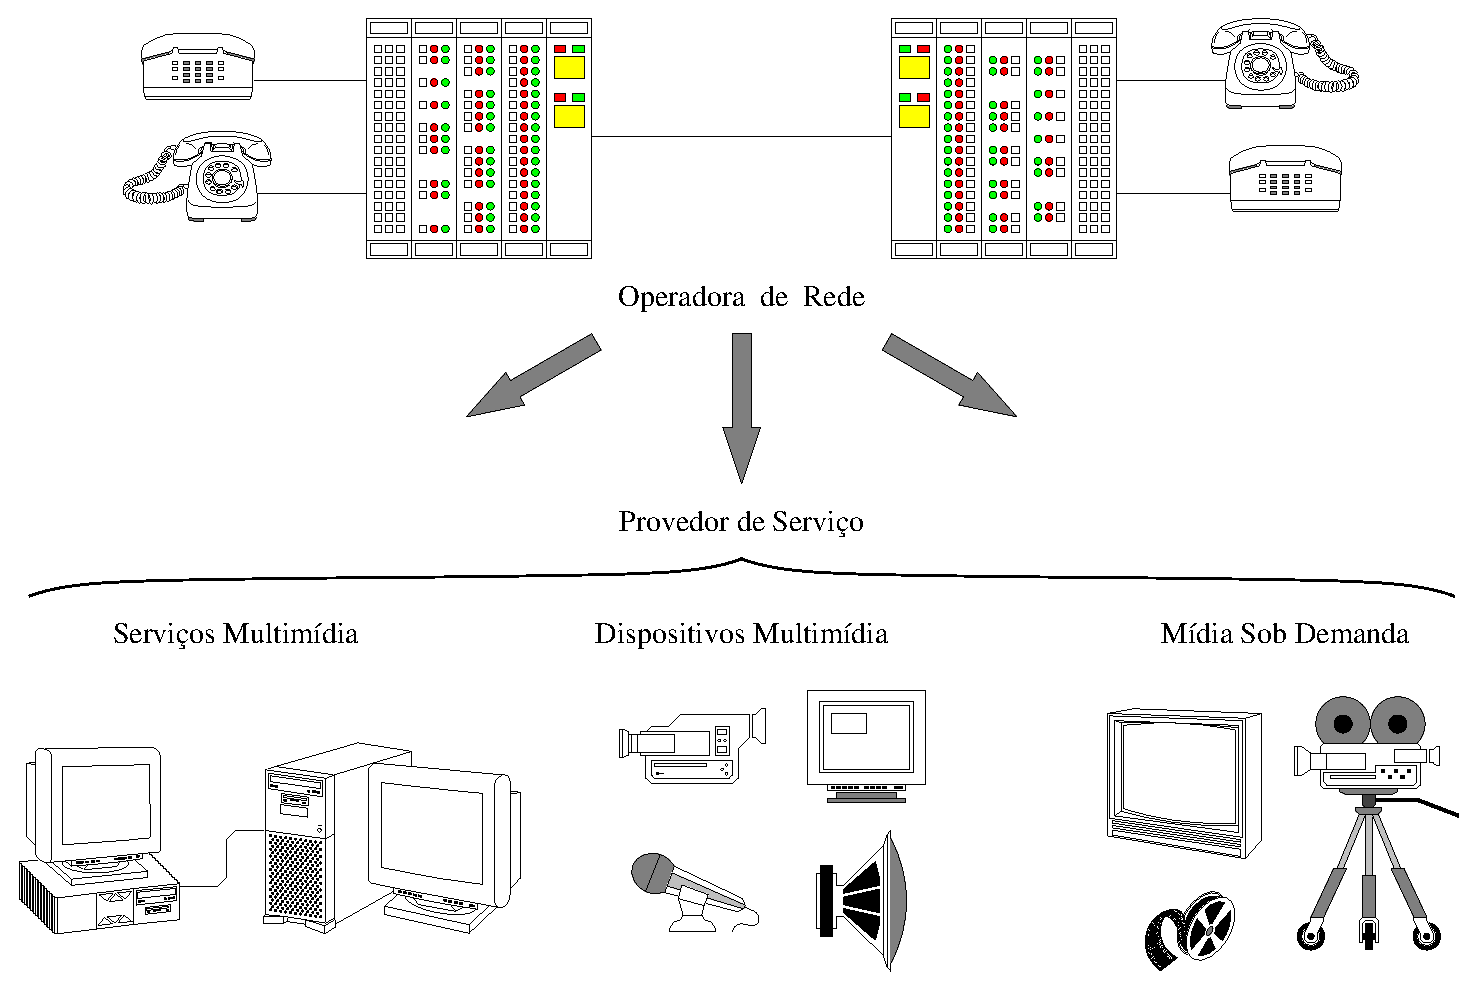
\includegraphics[width=0.55\textwidth]{./CapituloExemplo/figura1}%% Dimens\~oes e localiza\c{c}\~ao
\fonte{\citet{Larsson2003}.}%% Fonte
\end{figure}

Figuras em formato GIF, JPEG e BMP podem ser convertidas para o formato \gls{eps} atrav\'es do aplicativo ``xv''. O ``xv'' n\~ao lista o formato \gls{eps} dentre aqueles que \'e capaz de manipular. Entretanto, selecionando-se o formato \textit{PostScript} e fornecendo-se a extens\~ao \texttt{eps} ao nome do arquivo, o formato \gls{eps} \'e gerado.

O ambiente \texttt{picture} permite a programa\c{c}\~ao de imagens diretamente no \gls{latex}\index{LaTeX@\latex}, conforme exemplo apresentado na \autoref{fig:figura2}.

\begin{figure}[Htb]%% Ambiente figure
\captionsetup{width=8cm}%% Largura da legenda
\caption{Exemplo de figura criada a partir do ambiente \texttt{picture}.}%% Legenda
\label{fig:figura2}%% R\'otulo
\setlength{\unitlength}{1cm}%% Unidade de comprimento
\begin{picture}(8,5)(-4,-2.5)%% Ambiente picture
\put(-4,0){\vector(1,0){8}}
\put(3.75,-0.25){$\chi$}
\put(0,-2.5){\vector(0,1){5}}
\multiput(-4,1)(0.4,0){20}{\line(1,0){0.2}}
\multiput(-4,-1)(0.4,0){20}{\line(1,0){0.2}}
\put(0.25,2.25){$\beta \equiv v / c = \tanh \chi$}
\qbezier(0,0)(0.8853,0.8853)(2,0.9640)
\qbezier(0,0)(-0.8853,-0.8853)(-2,-0.9640)
\end{picture}
\fonte{Autoria pr\'opria.}%% Fonte
\end{figure}

A \autoref{fig:subfigure} apresenta um exemplo usando o pacote \texttt{subfigure} com legendas usando o pacote \texttt{subcaption}. \'E  poss\'{\i}vel referenciar cada uma das sub-figuras, no qual, a sua refer\^encia alfab\'etica aparece entre par\^enteses: \autoref{fig:subfigure_a} e \autoref{fig:subfigure_b}.

\begin{figure}[!ht]
\centering
\caption{Exemplo de Subfigure} 
\label{fig:subfigure}
\begin{subfigure}[t]{.45\textwidth}
	\centering
	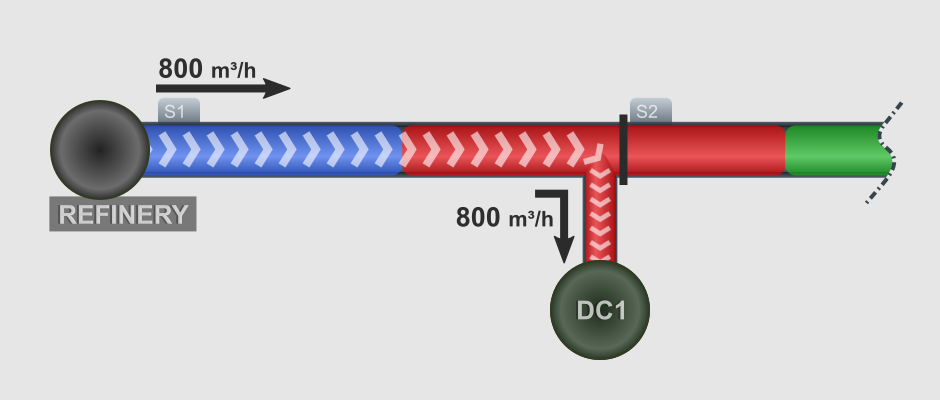
\includegraphics[width=\textwidth]{./CapituloExemplo/subfigure-a.png}
	\caption{Figura A}
	\label{fig:subfigure_a}
\end{subfigure}
\qquad
\begin{subfigure}[t]{.45\textwidth}
	\centering
	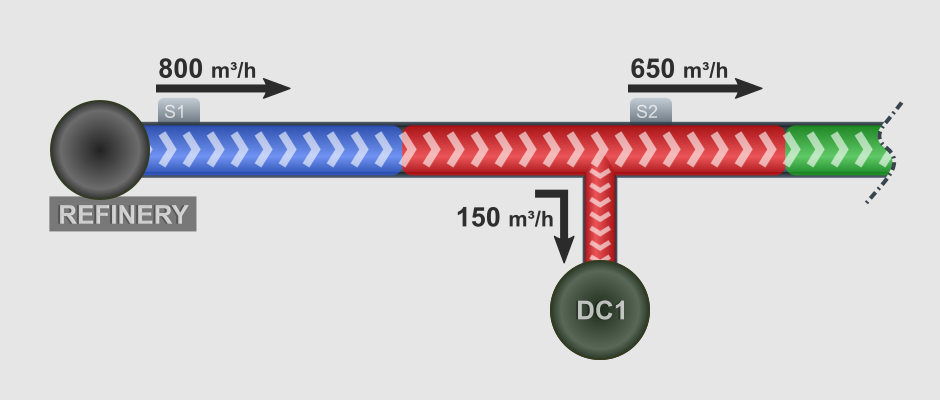
\includegraphics[width=\textwidth]{./CapituloExemplo/subfigure-b.png}  
	\caption{Figura B}
	\label{fig:subfigure_b}
\end{subfigure}
\fonte{\citet{Meira2020}} %citeonline{meira2020}
\end{figure}

%% T\'{\i}tulo e r\'otulo de se\c{c}\~ao (r\'otulos n\~ao devem conter caracteres especiais, acentuados ou cedilha)
\subsection{Fotografias}\label{sec:fotografias}

Um exemplo deste tipo de ilustra\c{c}\~ao \'e apresentado na \autoref{foto:foto1}.

\begin{photograph}[Htb]%% Ambiente photograph
\captionsetup{width=0.6\textwidth}%% Largura da legenda
\caption{Camale\~ao pantera fotografado por Joel Sartore, National Geographic.}%% Legenda
\label{foto:foto1}%% R\'otulo
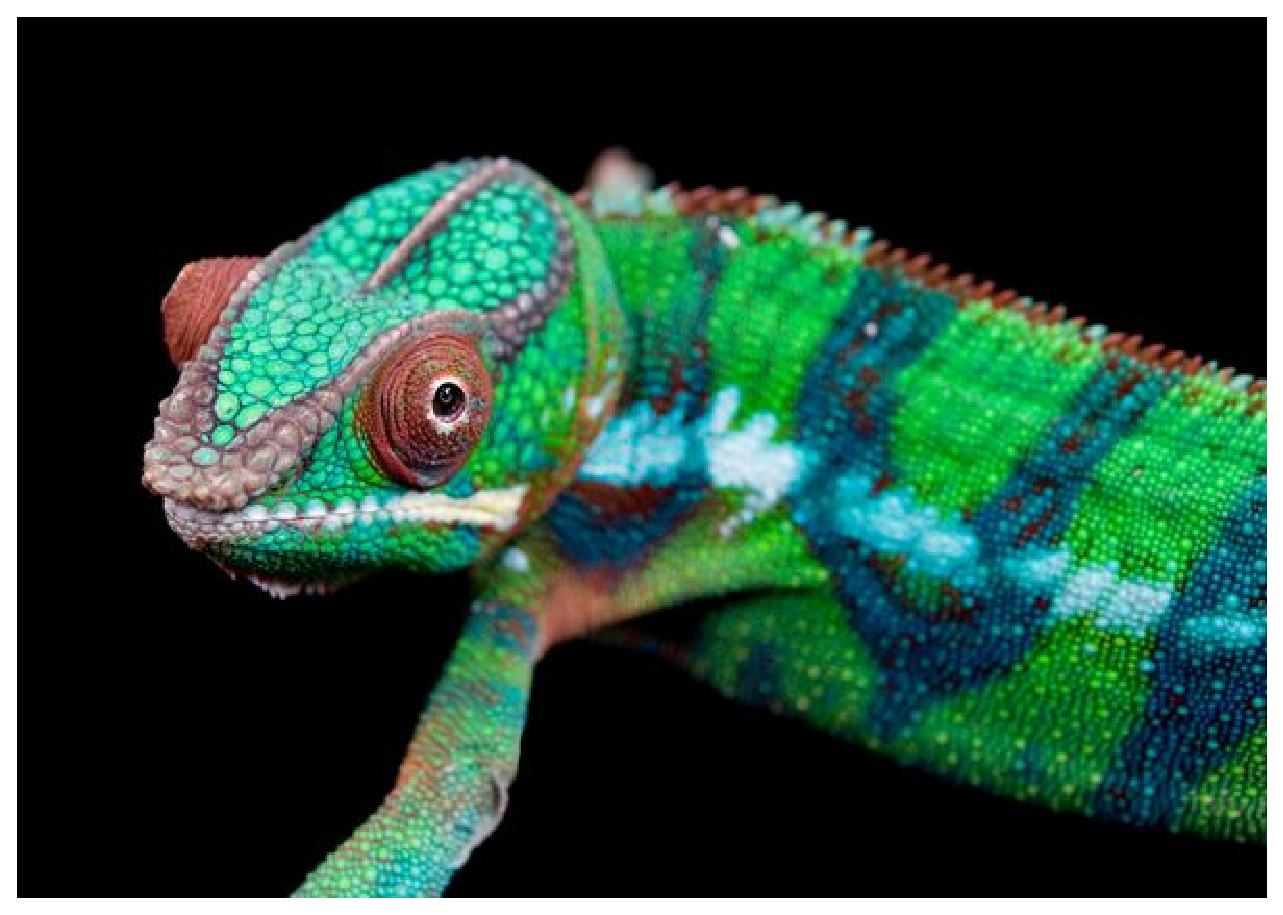
\includegraphics[width=0.6\textwidth]{./CapituloExemplo/foto1}%% Dimens\~oes e localiza\c{c}\~ao
\fonte{\citet{Sartore2013}.}%% Fonte
\end{photograph}

Outro exemplo deste tipo de ilustra\c{c}\~ao \'e apresentado na \autoref{foto:foto2}.

\begin{photograph}[Htb]%% Ambiente photograph
\captionsetup{width=0.6\textwidth}%% Largura da legenda
\caption{Fotografia da erup\c{c}\~ao vulc\^anica em 1982 do Galungung, Indon\'esia (com descargas de raios), produzida pelo Servi\c{c}o Geol\'ogico dos Estados Unidos da Am\'erica.}%% Legenda
\label{foto:foto2}%% R\'otulo
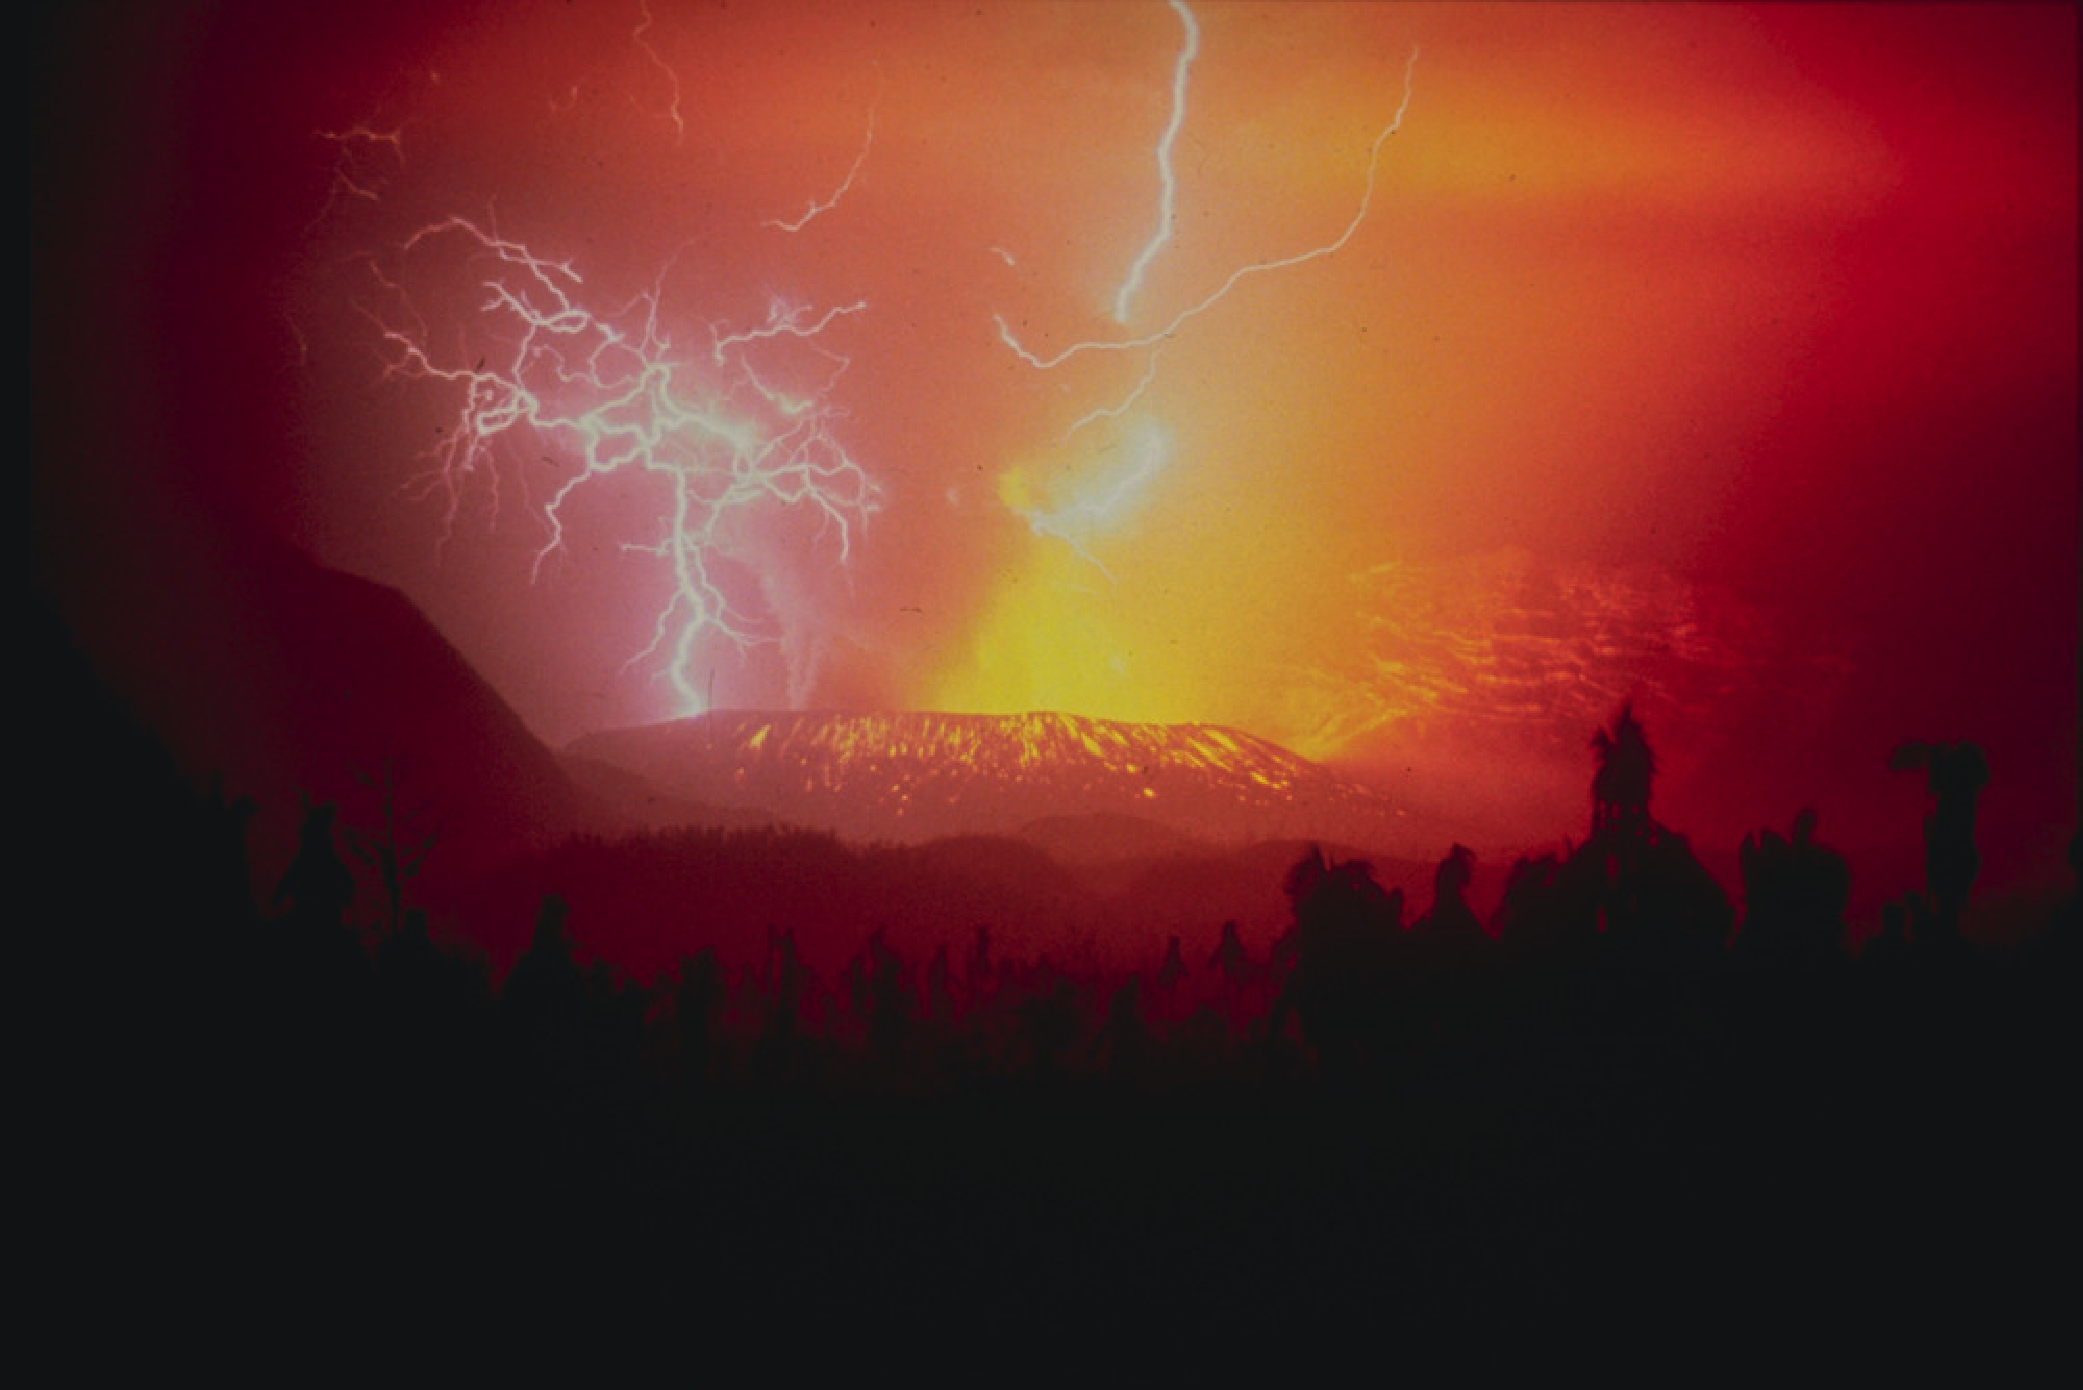
\includegraphics[width=0.6\textwidth]{./CapituloExemplo/foto2}%% Dimens\~oes e localiza\c{c}\~ao
\fonte{\citet{Hadian1982}.}%% Fonte
\end{photograph}

%% T\'{\i}tulo e r\'otulo de se\c{c}\~ao (r\'otulos n\~ao devem conter caracteres especiais, acentuados ou cedilha)
\subsection{Gr\'aficos}\label{sec:graficos}

Gr\'aficos s\~ao gerados com aplicativos capazes de exportar nos formatos \gls{ps} ou \gls{eps}. A ferramenta ``gnuplot'' \'e uma das mais utilizadas para a gera\c{c}\~ao de gr\'aficos (\url{http://www.gnuplot.info/}). Uma vez no formato \gls{eps}, gr\'aficos s\~ao inseridos no texto tal como figuras (veja \autoref{gra:grafico1}).

\begin{graph}[Htb]%% Ambiente graph
\captionsetup{width=0.6\textwidth}%% Largura da legenda
\caption{Exemplo de gr\'afico produzido em ``gnuplot''.}%% Legenda
\label{gra:grafico1}%% R\'otulo
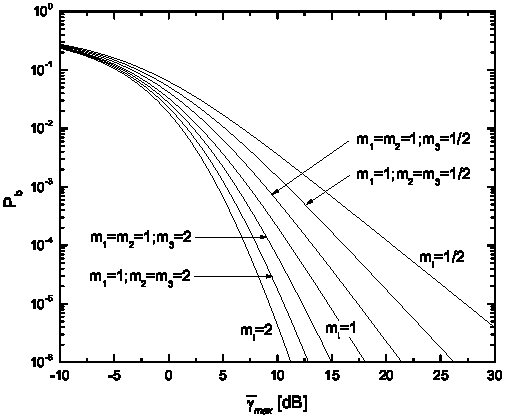
\includegraphics[width=0.6\textwidth]{./CapituloExemplo/grafico1}%% Dimens\~oes e localiza\c{c}\~ao
\fonte{\citet{Faina2001}.}%% Fonte
\end{graph}

No \autoref{gra:grafico2} \'e apresentado um exemplo de gr\'afico produzido em ``Excel''.

\begin{graph}[Htb]%% Ambiente graph
\captionsetup{width=0.6\textwidth}%% Largura da legenda
\caption{Exemplo de gr\'afico produzido em ``Excel''.}%% Legenda
\label{gra:grafico2}%% R\'otulo
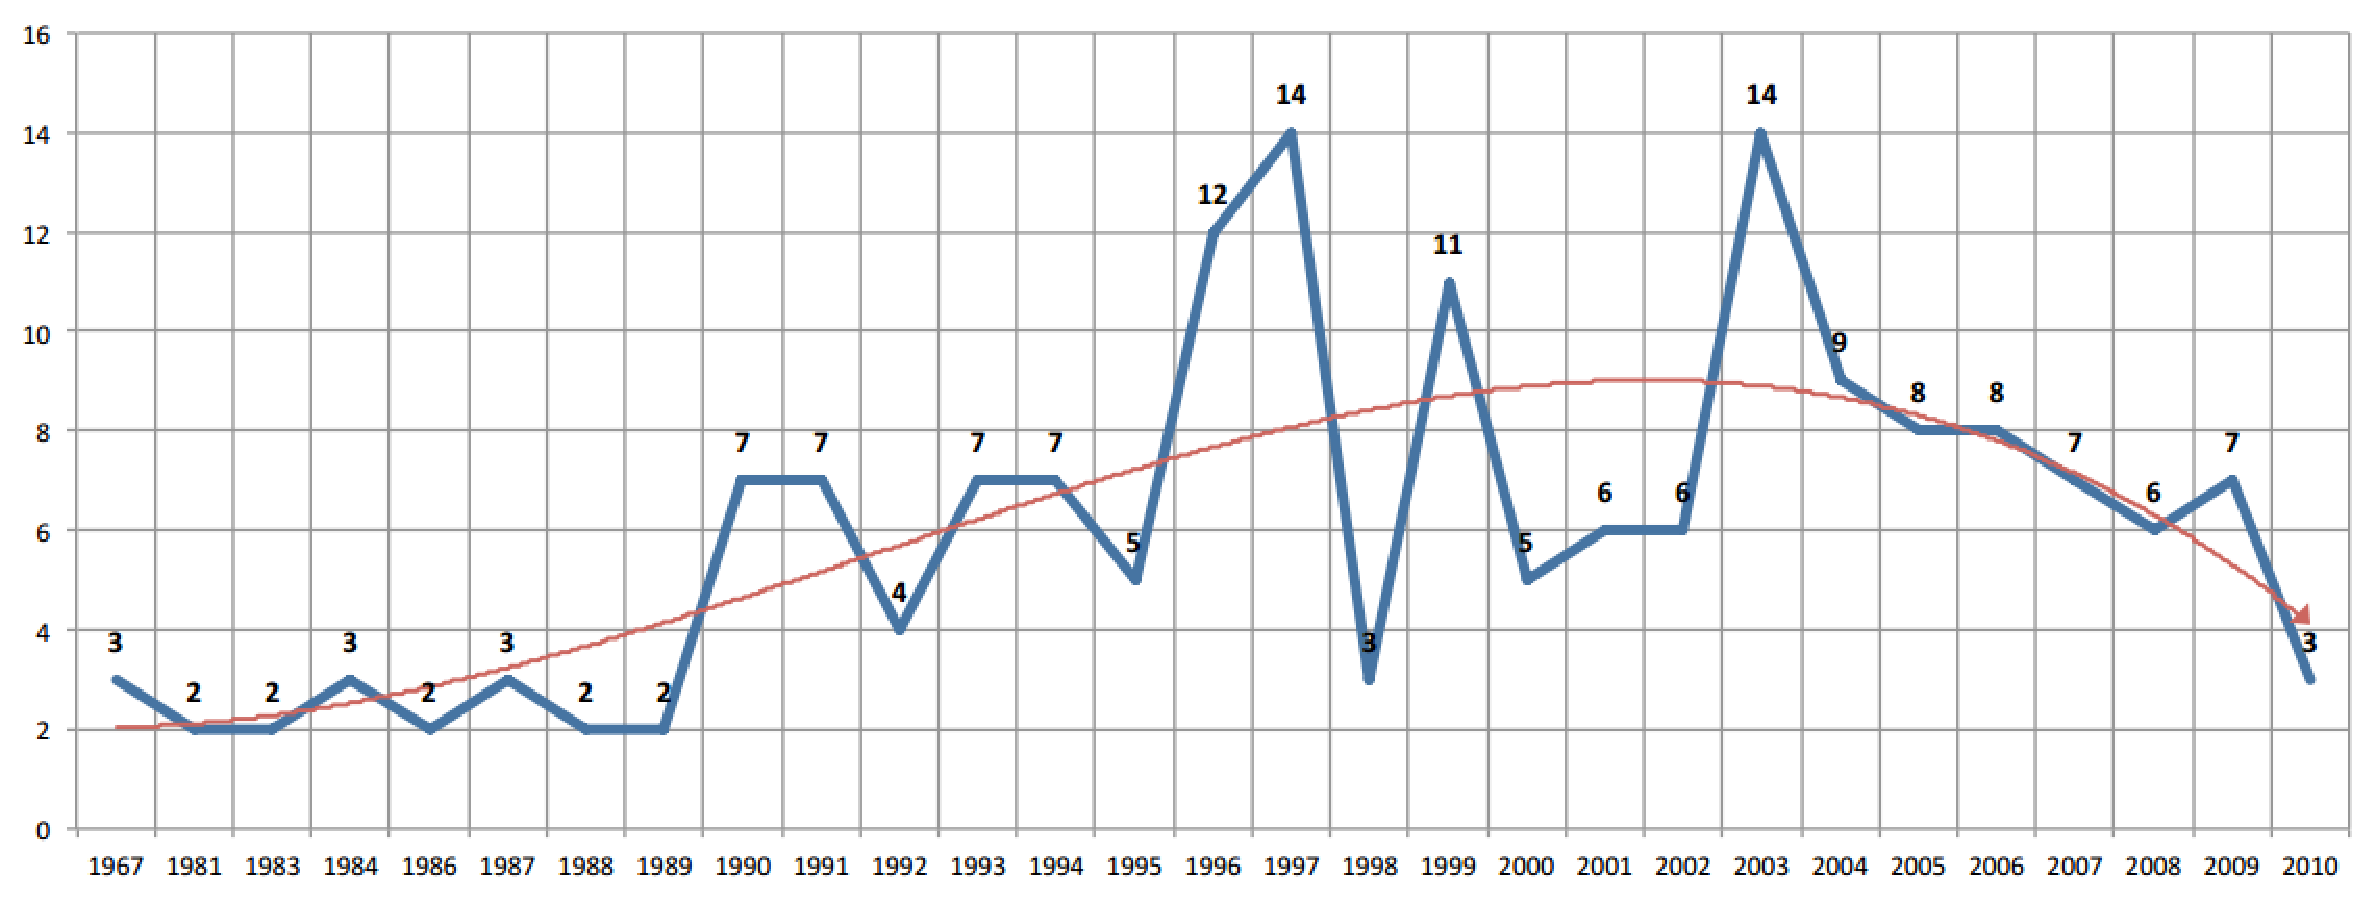
\includegraphics[width=0.6\textwidth]{./CapituloExemplo/grafico2}%% Dimens\~oes e localiza\c{c}\~ao
\fonte{\citeonline[p. 24]{Araujo2012}.}%% Fonte
\end{graph}

O ambiente \texttt{minipage} pode ser usado para inserir textos ou outros elementos em quadros com tamanhos e posi\c{c}\~oes controladas, conforme exemplos apresentados no \autoref{gra:minipagegrafico1} e no \autoref{gra:minipagegrafico2}.

\begin{graph}[Htb]%% Ambiente graph
\begin{minipage}[t]{0.395\textwidth}%% Ambiente minipage
\centering%% Centralizado
\captionsetup{width=0.85\textwidth}%% Largura da legenda
\caption{Gr\'afico 1 do ambiente \texttt{minipage}.}%% Legenda
\label{gra:minipagegrafico1}%% R\'otulo
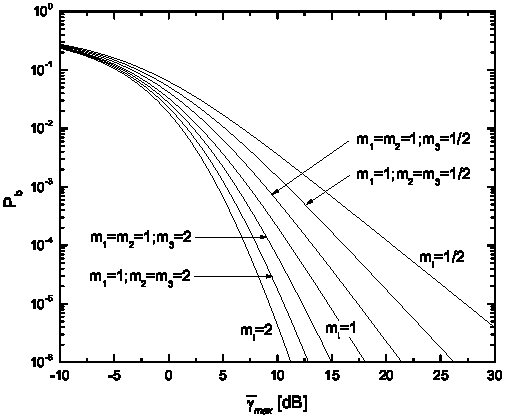
\includegraphics[width=0.85\textwidth]{./CapituloExemplo/grafico1}%% Dimens\~oes e localiza\c{c}\~ao
\fonte{\citet{Faina2001}.}%% Fonte
\end{minipage}
\hfill
\begin{minipage}[t]{0.595\textwidth}%% Ambiente minipage
\centering%% Centralizado
\captionsetup{width=0.95\textwidth}%% Largura da legenda
\caption{Gr\'afico 2 do ambiente \texttt{minipage}.}%% Legenda
\label{gra:minipagegrafico2}%% R\'otulo
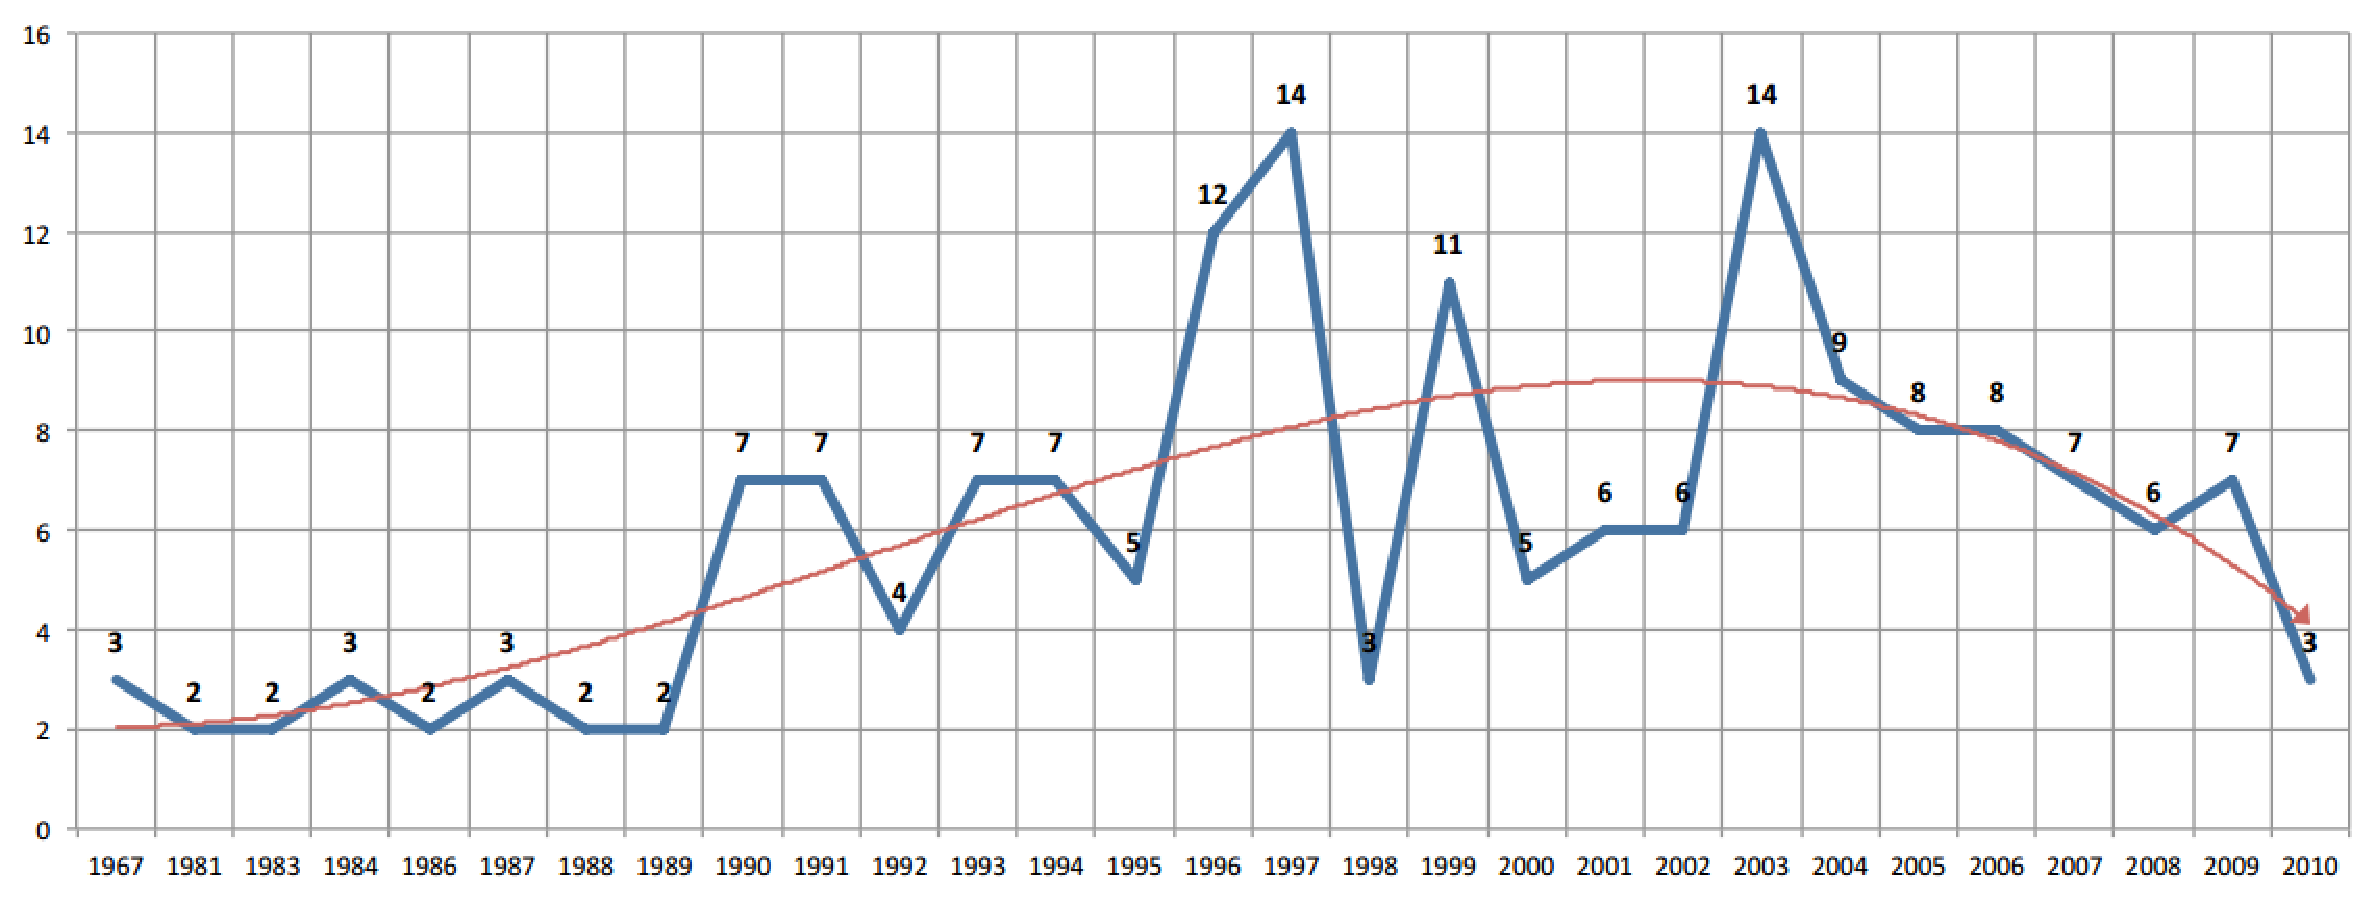
\includegraphics[width=0.95\textwidth]{./CapituloExemplo/grafico2}%% Dimens\~oes e localiza\c{c}\~ao
\fonte{\citeonline[p. 24]{Araujo2012}}%% Fonte
\end{minipage}
\label{gra:minipagegraficos}
\end{graph}

%% T\'{\i}tulo e r\'otulo de se\c{c}\~ao (r\'otulos n\~ao devem conter caracteres especiais, acentuados ou cedilha)
\subsection{Quadros}\label{sec:quadros}

Um exemplo deste tipo de ilustra\c{c}\~ao \'e apresentado no \autoref{quad:quadro1}.

\begin{tabframed}[Htb]%% Ambiente tabframed
\captionsetup{width=0.5\textwidth}%% Largura da legenda
\caption{Compostos org\^anicos: f\'ormulas estruturais e principais classes.}%% Legenda
\label{quad:quadro1}%% R\'otulo
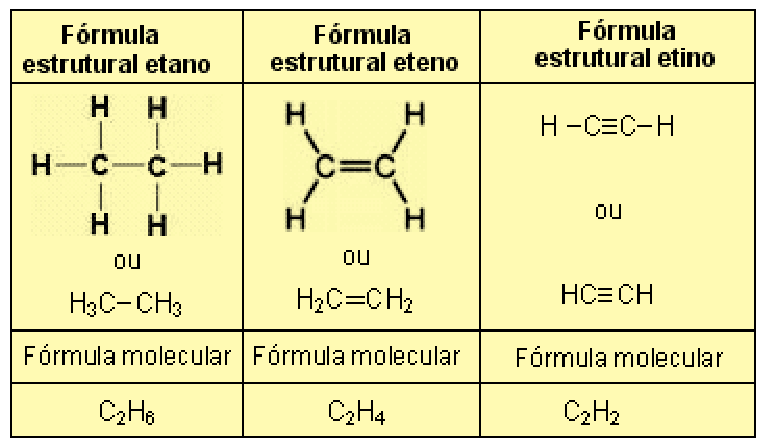
\includegraphics[width=0.5\textwidth]{./CapituloExemplo/quadro1}%% Dimens\~oes e localiza\c{c}\~ao
\fonte{\citet{daSilva2009}.}%% Fonte
\end{tabframed}

Outro exemplo deste tipo de ilustra\c{c}\~ao \'e apresentado no \autoref{quad:quadro2}.

\begin{tabframed}[Htb]%% Ambiente tabframed
\captionsetup{width=0.7\textwidth}%% Largura da legenda
\caption{Modelos de maturidade para a gest\~ao da cadeia de suprimentos.}%% Legenda
\label{quad:quadro2}%% R\'otulo
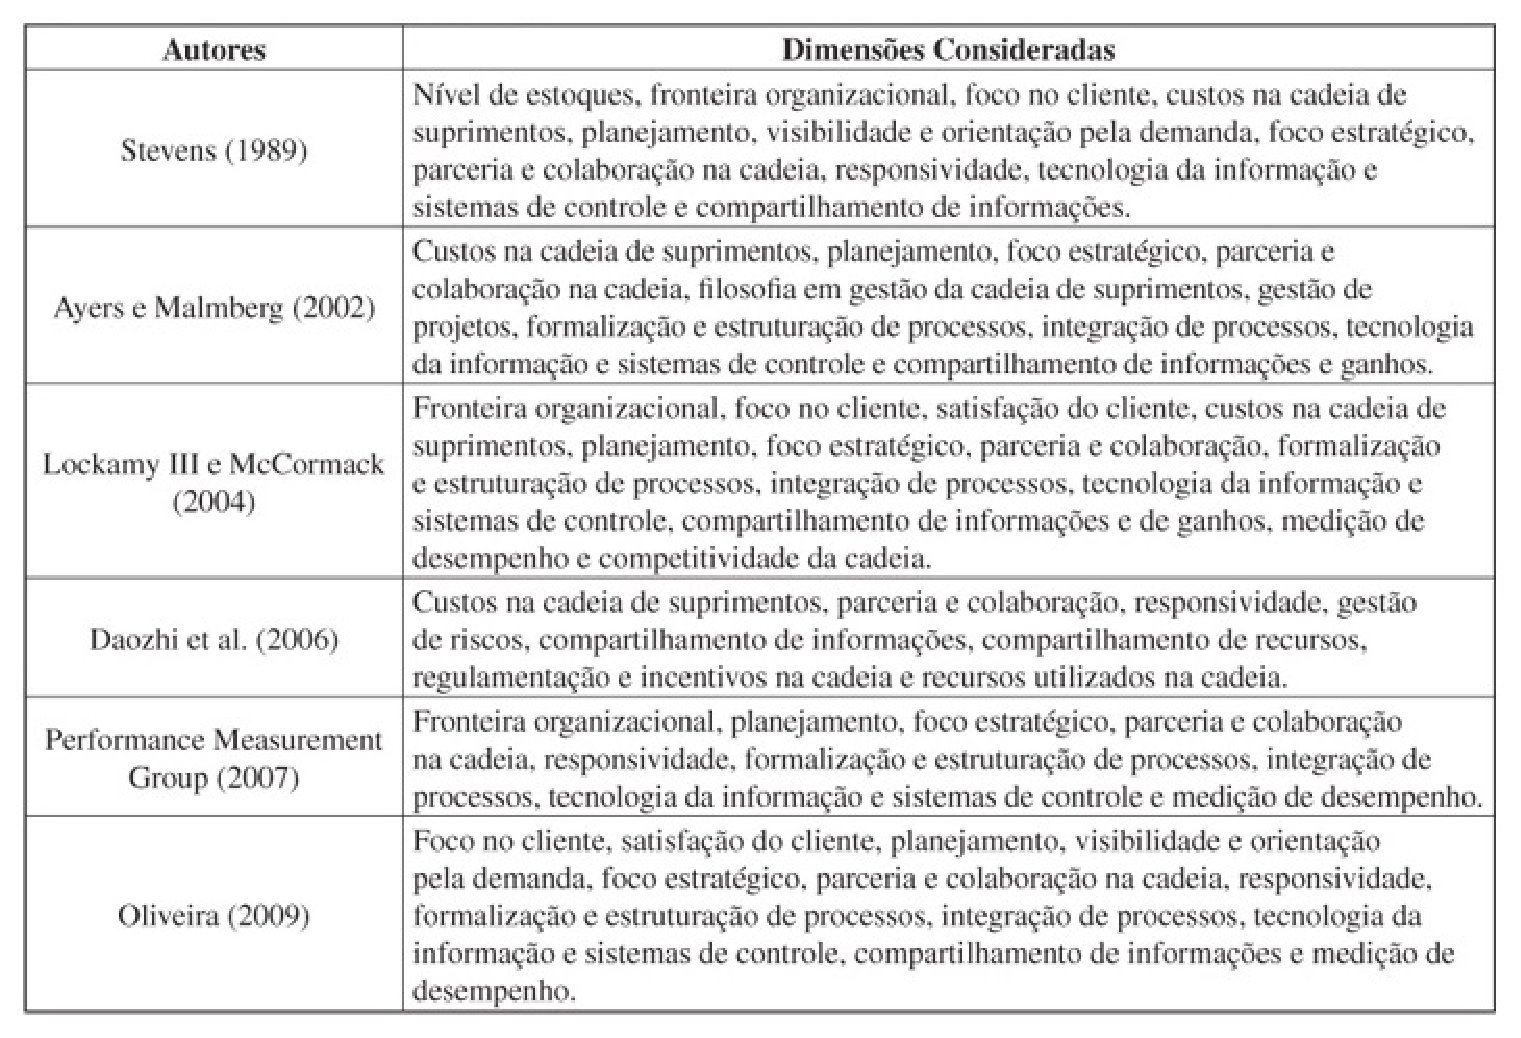
\includegraphics[width=0.7\textwidth]{./CapituloExemplo/quadro2}%% Dimens\~oes e localiza\c{c}\~ao
\fonte{\citet{Frederico2012}.}%% Fonte
\end{tabframed}

Os quadros n\~ao devem ser chamados de tabelas, uma vez que se diferenciam destas por apresentarem as laterais fechadas e o conte\'udo n\~ao num\'erico.

%% T\'{\i}tulo e r\'otulo de se\c{c}\~ao (r\'otulos n\~ao devem conter caracteres especiais, acentuados ou cedilha)
\section{Tabelas}\label{sec:tabelas}

Tabelas s\~ao constru\'{\i}das com comandos pr\'oprios do \gls{latex}\index{LaTeX@\latex}. Por exemplo, a \autoref{tab:tabela1} foi constru\'{\i}da desta forma.

\begin{table}[Htb]%% Ambiente table
\caption{Primeiro exemplo de tabela com uma legenda contendo um texto muito longo que pode ocupar mais de uma linha.}%% Legenda
\label{tab:tabela1}%% R\'otulo
\begin{tabularx}{\textwidth}{@{\extracolsep{\fill}}llll}%% Ambiente tabularx
\toprule
$\bsym{L}$ & $\bsym{L^2}$ & $\bsym{L^3}$ & $\bsym{L^4}$ \\
\SI{}{[m]} & \SI{}{[m^2]} & \SI{}{[m^3]} & \SI{}{[m^4]} \\ \midrule
1          & 1            & 1            & 1            \\
2          & 4            & 8            & 16           \\
3          & 9            & 27           & 81           \\
4          & 16           & 64           & 256          \\
5          & 25           & 125          & 625          \\ \bottomrule
\end{tabularx}
\fonte{Autoria pr\'opria.}%% Fonte
\end{table}

A \autoref{tab:tabela2} \'e um exemplo de tabela que ocupa mais de uma p\'agina e que foi constru\'{\i}da pelo \gls{latex}\index{LaTeX@\latex} utilizando o pacote \texttt{longtable}.

\begin{longtable}{@{\extracolsep{\fill}}lll}%% Ambiente longtable
\caption{Poss\'{\i}veis tr\'{\i}plices para grade altamente vari\'avel.\label{tab:tabela2}} \\%% Legenda e r\'otulo
\toprule
\textbf{Tempo (s)} & \textbf{Tr\'{\i}plice escolhida} & \textbf{Outras poss\'{\i}veis tr\'{\i}plices} \\
\midrule
\endfirsthead%% Encerra cabe\c{c}alho da primeira p\'agina
\caption[]{Poss\'{\i}veis tr\'{\i}plices para grade altamente vari\'avel.} \\%% Legenda
\multicolumn{3}{r}{\textbf{(continua\c{c}\~ao)}} \\
\toprule
\textbf{Tempo (s)} & \textbf{Tr\'{\i}plice escolhida} & \textbf{Outras poss\'{\i}veis tr\'{\i}plices} \\
\midrule
\endhead%% Encerra cabe\c{c}alho das demais p\'aginas
\midrule
\multicolumn{3}{r}{\textbf{(continua)}} \\
\endfoot%% Encerra rodap\'e das demais p\'aginas
\bottomrule
\\[-0.5\linha]
\caption*{\nomefonte: Adaptado de \citet{Smallen2014}.} \\
\endlastfoot%% Encerra rodap\'e da \'ultima p\'agina
0      & (1, 11, 13725) & (1, 12, 10980), (1, 13, 8235), (2, 2, 0), (3, 1, 0) \\
2745   & (1, 12, 10980) & (1, 13, 8235), (2, 2, 0), (2, 3, 0), (3, 1, 0)      \\
5490   & (1, 12, 13725) & (2, 2, 2745), (2, 3, 0), (3, 1, 0)                  \\
8235   & (1, 12, 16470) & (1, 13, 13725), (2, 2, 2745), (2, 3, 0), (3, 1, 0)  \\
10980  & (1, 12, 16470) & (1, 13, 13725), (2, 2, 2745), (2, 3, 0), (3, 1, 0)  \\
13725  & (1, 12, 16470) & (1, 13, 13725), (2, 2, 2745), (2, 3, 0), (3, 1, 0)  \\
16470  & (1, 13, 16470) & (2, 2, 2745), (2, 3, 0), (3, 1, 0)                  \\
19215  & (1, 12, 16470) & (1, 13, 13725), (2, 2, 2745), (2, 3, 0), (3, 1, 0)  \\
21960  & (1, 12, 16470) & (1, 13, 13725), (2, 2, 2745), (2, 3, 0), (3, 1, 0)  \\
24705  & (1, 12, 16470) & (1, 13, 13725), (2, 2, 2745), (2, 3, 0), (3, 1, 0)  \\
27450  & (1, 12, 16470) & (1, 13, 13725), (2, 2, 2745), (2, 3, 0), (3, 1, 0)  \\
30195  & (2, 2, 2745)   & (2, 3, 0), (3, 1, 0)                                \\
32940  & (1, 13, 16470) & (2, 2, 2745), (2, 3, 0), (3, 1, 0)                  \\
35685  & (1, 13, 13725) & (2, 2, 2745), (2, 3, 0), (3, 1, 0)                  \\
38430  & (1, 13, 10980) & (2, 2, 2745), (2, 3, 0), (3, 1, 0)                  \\
41175  & (1, 12, 13725) & (1, 13, 10980), (2, 2, 2745), (2, 3, 0), (3, 1, 0)  \\
43920  & (1, 13, 10980) & (2, 2, 2745), (2, 3, 0), (3, 1, 0)                  \\
46665  & (2, 2, 2745)   & (2, 3, 0), (3, 1, 0)                                \\
49410  & (2, 2, 2745)   & (2, 3, 0), (3, 1, 0)                                \\
52155  & (1, 12, 16470) & (1, 13, 13725), (2, 2, 2745), (2, 3, 0), (3, 1, 0)  \\
54900  & (1, 13, 13725) & (2, 2, 2745), (2, 3, 0), (3, 1, 0)                  \\
57645  & (1, 13, 13725) & (2, 2, 2745), (2, 3, 0), (3, 1, 0)                  \\
60390  & (1, 12, 13725) & (2, 2, 2745), (2, 3, 0), (3, 1, 0)                  \\
63135  & (1, 13, 16470) & (2, 2, 2745), (2, 3, 0), (3, 1, 0)                  \\
65880  & (1, 13, 16470) & (2, 2, 2745), (2, 3, 0), (3, 1, 0)                  \\
68625  & (2, 2, 2745)   & (2, 3, 0), (3, 1, 0)                                \\
71370  & (1, 13, 13725) & (2, 2, 2745), (2, 3, 0), (3, 1, 0)                  \\
74115  & (1, 12, 13725) & (2, 2, 2745), (2, 3, 0), (3, 1, 0)                  \\
76860  & (1, 13, 13725) & (2, 2, 2745), (2, 3, 0), (3, 1, 0)                  \\
79605  & (1, 13, 13725) & (2, 2, 2745), (2, 3, 0), (3, 1, 0)                  \\
82350  & (1, 12, 13725) & (2, 2, 2745), (2, 3, 0), (3, 1, 0)                  \\
85095  & (1, 12, 13725) & (1, 13, 10980), (2, 2, 2745), (2, 3, 0), (3, 1, 0)  \\
87840  & (1, 13, 16470) & (2, 2, 2745), (2, 3, 0), (3, 1, 0)                  \\
90585  & (1, 13, 16470) & (2, 2, 2745), (2, 3, 0), (3, 1, 0)                  \\
93330  & (1, 13, 13725) & (2, 2, 2745), (2, 3, 0), (3, 1, 0)                  \\
96075  & (1, 13, 16470) & (2, 2, 2745), (2, 3, 0), (3, 1, 0)                  \\
98820  & (1, 13, 16470) & (2, 2, 2745), (2, 3, 0), (3, 1, 0)                  \\
101565 & (1, 13, 13725) & (2, 2, 2745), (2, 3, 0), (3, 1, 0)                  \\
104310 & (1, 13, 16470) & (2, 2, 2745), (2, 3, 0), (3, 1, 0)                  \\
107055 & (1, 13, 13725) & (2, 2, 2745), (2, 3, 0), (3, 1, 0)                  \\
109800 & (1, 13, 13725) & (2, 2, 2745), (2, 3, 0), (3, 1, 0)                  \\
112545 & (1, 12, 16470) & (1, 13, 13725), (2, 2, 2745), (2, 3, 0), (3, 1, 0)  \\
115290 & (1, 13, 16470) & (2, 2, 2745), (2, 3, 0), (3, 1, 0)                  \\
118035 & (1, 13, 13725) & (2, 2, 2745), (2, 3, 0), (3, 1, 0)                  \\
120780 & (1, 13, 16470) & (2, 2, 2745), (2, 3, 0), (3, 1, 0)                  \\
123525 & (1, 13, 13725) & (2, 2, 2745), (2, 3, 0), (3, 1, 0)                  \\
126270 & (1, 12, 16470) & (1, 13, 13725), (2, 2, 2745), (2, 3, 0), (3, 1, 0)  \\
129015 & (2, 2, 2745)   & (2, 3, 0), (3, 1, 0)                                \\
131760 & (2, 2, 2745)   & (2, 3, 0), (3, 1, 0)                                \\
134505 & (1, 13, 16470) & (2, 2, 2745), (2, 3, 0), (3, 1, 0)                  \\
137250 & (1, 13, 13725) & (2, 2, 2745), (2, 3, 0), (3, 1, 0)                  \\
139995 & (2, 2, 2745)   & (2, 3, 0), (3, 1, 0)                                \\
142740 & (2, 2, 2745)   & (2, 3, 0), (3, 1, 0)                                \\
145485 & (1, 12, 16470) & (1, 13, 13725), (2, 2, 2745), (2, 3, 0), (3, 1, 0)  \\
148230 & (2, 2, 2745)   & (2, 3, 0), (3, 1, 0)                                \\
150975 & (1, 13, 16470) & (2, 2, 2745), (2, 3, 0), (3, 1, 0)                  \\
153720 & (1, 12, 13725) & (2, 2, 2745), (2, 3, 0), (3, 1, 0)                  \\
156465 & (1, 13, 13725) & (2, 2, 2745), (2, 3, 0), (3, 1, 0)                  \\
159210 & (1, 13, 13725) & (2, 2, 2745), (2, 3, 0), (3, 1, 0)                  \\
161955 & (1, 13, 16470) & (2, 2, 2745), (2, 3, 0), (3, 1, 0)                  \\
164700 & (1, 13, 13725) & (2, 2, 2745), (2, 3, 0), (3, 1, 0)                  \\
\end{longtable}

Tabelas criadas em planilhas do ``Excel'' podem ser convertidas em tabelas \gls{latex}\index{LaTeX@\latex} atrav\'es do suplemento ``Excel-to-LaTeX'', dispon\'{\i}vel em \url{http://www.ctan.org/pkg/excel2latex}.

%% T\'{\i}tulo e r\'otulo de se\c{c}\~ao (r\'otulos n\~ao devem conter caracteres especiais, acentuados ou cedilha)
\section{Abreviaturas, Siglas e Acr\^onimos}\label{sec:acronimos}

\gls{latex}\index{LaTeX@\latex} gera automaticamente a lista de abreviaturas, siglas e acr\^onimos atrav\'es do pacote \texttt{glossaries}. As abreviaturas, siglas e acr\^onimos devem ser definidos no arquivo \texttt{entradas-acronimos.tex}, no diret\'orio ``PreTexto'', com os comandos:

\begin{SingleSpacing}%% Ambiente SingleSpacing
\begin{verbatim}
\abreviatura{r\'otulo}{representa\c{c}\~ao}{defini\c{c}\~ao}
\sigla{r\'otulo}{representa\c{c}\~ao}{defini\c{c}\~ao}
\acronimo{r\'otulo}{representa\c{c}\~ao}{defini\c{c}\~ao}
\end{verbatim}
\end{SingleSpacing}

Para que a abreviatura, sigla ou acr\^onimo seja apresentada em alguma parte do texto do documento use o comando \verb|\gls{r\'otulo}|, por exemplo, as abreviaturas \gls{art.}, \gls{cap.} e \gls{sec.} foram geradas pelos comandos \verb|\gls{art.}, \gls{cap.} e \gls{sec.}|, respectivamente. Mais detalhes dos comandos do pacote \texttt{glossaries} podem ser encontrados em: \url{http://mirrors.ctan.org/macros/latex/contrib/glossaries/glossaries-user.pdf}.

Outra op\c{c}\~ao para gerar a lista de abreviaturas, siglas e acr\^onimos \'e atrav\'es da edi\c{c}\~ao manual do arquivo \texttt{lista-acronimos.tex} no diret\'orio ``PreTexto''.

%% T\'{\i}tulo e r\'otulo de se\c{c}\~ao (r\'otulos n\~ao devem conter caracteres especiais, acentuados ou cedilha)
\section{S\'{\i}mbolos}\label{sec:simbolos}

\gls{latex}\index{LaTeX@\latex} gera automaticamente a lista de s\'{\i}mbolos atrav\'es do pacote \texttt{nomencl}. Ao redigir um s\'{\i}mbolo pela primeira vez em qualquer parte do texto com o comando \verb|\nomenclature[prefixo]{s\'{\i}mbolo}{descri\c{c}\~ao \nomunit{unidade}}|, \'e gerada uma entrada para a lista de s\'{\i}mbolos. Veja exemplos deste comando no arquivo fonte deste cap\'{\i}tulo. Os elementos da lista de s\'{\i}mbolos s\~ao ordenados a depender da primeira letra atribu\'{\i}da ao prefixo e classificadas em:

\begin{itemize}%% Lista de itens
\item A~-~Letras Latinas.
\item B~-~Letras Gregas.
\item C~-~Sobrescritos.
\item D~-~Subscritos.
\item E~-~Nota\c{c}\~oes.
\item F~-~\'Indices e Conjuntos
\item G~-~Par\^ametros
\item H~-~Vari\'aveis cont\'{\i}nuas
\item I~-~Vari\'aveis inteiras
\item J~-~Vari\'aveis bin\'arias
\end{itemize}

Outra op\c{c}\~ao ao comando \verb|\nomenclature| \'e o uso dos atalhos:

\begin{SingleSpacing}%% Ambiente SingleSpacing
\begin{verbatim}
\letralatina{prefixo}{s\'{\i}mbolo}{descri\c{c}\~ao}{unidade}
\letragrega{prefixo}{s\'{\i}mbolo}{descri\c{c}\~ao}{unidade}
\sobrescrito{prefixo}{s\'{\i}mbolo}{descri\c{c}\~ao}{unidade}
\subscrito{prefixo}{s\'{\i}mbolo}{descri\c{c}\~ao}{unidade}
\notacao{prefixo}{s\'{\i}mbolo}{descri\c{c}\~ao}{unidade}
\notacaois{s\'{\i}mbolo}{descri\c{c}\~ao}{unidade}
\notacaoparam{s\'{\i}mbolo}{descri\c{c}\~ao}{unidade}
\notacaofloatvar{s\'{\i}mbolo}{descri\c{c}\~ao}{unidade}
\notacaointvar{s\'{\i}mbolo}{descri\c{c}\~ao}{unidade}
\notacaobinvar{s\'{\i}mbolo}{descri\c{c}\~ao}{unidade}
\end{verbatim}
\end{SingleSpacing}

\noindent Neste caso a atribui\c{c}\~ao da primeira letra do prefixo pode ser desprezada.

%% Letras Latinas [A]
\nomenclature[AA]{$A$}{\'Area \nomunit{m^2}}%%
\letralatina{L}{L}{Comprimento}{m}%%
\letralatina{R}{R}{Raio}{m}%%
%% Letras Gregas [B]
\nomenclature[Bmu]{$\mu$}{Viscosidade din\^amica \nomunit{kg/(m.s)}}%%
\letragrega{nu}{\nu}{Viscosidade cinem\'atica}{m^2/s}%%
\letragrega{pi}{\pi}{Pi (constante circular)}{rad}%%
\letragrega{rho}{\rho}{Massa espec\'{\i}fica}{kg/m^3}%%
\letragrega{sigma}{\sigma}{Tens\~ao superficial}{N/m}%%
%% Sobrescritos [C]
\nomenclature[C+]{$+$}{Passo de tempo posterior}%%
\sobrescrito{-}{-}{Passo de tempo anterior}{}%%
\sobrescrito{0}{0}{Valor inicial}{}%%
%% Subscritos [D]
\nomenclature[DG]{$G$}{Fase gasosa}%%
\subscrito{L}{L}{Fase l\'{\i}quida}{}%%
\subscrito{S}{S}{Fase s\'olida}{}%%
%% Nota\c{c}\~oes [E]
\nomenclature[EPsi_1]{$\overline{\Psi}$}{M\'edia temporal}%%
\notacao{Psi_2}{\langle \Psi \rangle}{M\'edia na se\c{c}\~ao transversal}{}%%
\notacao{Psi_3}{\langle\langle \Psi \rangle\rangle}{M\'edia na se\c{c}\~ao transversal ponderada}{}%%
%% Nota\c{c}\~oes [F]
\notacaois{Event_set}{e \in E}{Set of events}{}
\notacaois{Interval_set}{i \in I}{Set of intervals}{}
%% Nota\c{c}\~oes [H]
\notacaoparam{eps}{\varepsilon}{Small constant value}{}
\notacaoparam{lb}{L}{Lower bound value ($L \ll 0$)}{}
%% Nota\c{c}\~oes [I]
\notacaofloatvar{end}{e_{i}}{End of interval $i$}{h}
\notacaofloatvar{start}{s_{i}}{Start of interval $i$}{h}
%% Nota\c{c}\~oes [J]
\notacaointvar{e_i}{\phi_i}{Number of employees set to work during interval $i$}{}
%% Nota\c{c}\~oes [K]
\notacaobinvar{a_i}{a_{i}}{1 if the flow is active during interval $i$; 0 otherwise}{}

Mais detalhes dos comandos do pacote \texttt{nomencl} podem ser encontrados em: \url{http://tug.ctan.org/tex-archive/macros/latex/contrib/nomencl/nomencl.pdf}.

Outra op\c{c}\~ao para gerar a lista de s\'{\i}mbolos \'e atrav\'es da edi\c{c}\~ao manual do arquivo \texttt{lista-simbolos.tex} no diret\'orio ``PreTexto''.

%% T\'{\i}tulo e r\'otulo de se\c{c}\~ao (r\'otulos n\~ao devem conter caracteres especiais, acentuados ou cedilha)
\section{Inclus\~ao de Outros Arquivos}\label{sec:inclusao}

\'E uma boa pr\'atica dividir o seu documento em diversos arquivos, e n\~ao apenas escrever tudo em um \'unico. Esse recurso foi utilizado neste documento (veja \texttt{utfprct.tex}). Para incluir diferentes arquivos em um arquivo principal, de modo que cada arquivo inclu\'{\i}do fique em uma p\'agina diferente, utilize o comando:

\begin{SingleSpacing}%% Ambiente SingleSpacing
\begin{verbatim}
\include{documento-a-ser-incluido} %% Sem a extens\~ao .tex
\end{verbatim}
\end{SingleSpacing}

Para incluir documentos sem quebra de p\'aginas, utilize:

\begin{SingleSpacing}%% Ambiente SingleSpacing
\begin{verbatim}
\input{documento-a-ser-incluido}   %% Sem a extens\~ao .tex
\end{verbatim}
\end{SingleSpacing}

%% T\'{\i}tulo e r\'otulo de se\c{c}\~ao (r\'otulos n\~ao devem conter caracteres especiais, acentuados ou cedilha)
\section{Refer\^encias Bibliogr\'aficas}\label{sec:referencias}

A formata\c{c}\~ao das refer\^encias bibliogr\'aficas conforme as regras da \gls{abnt}\index{ABNT} s\~ao um dos principais objetivos do \gls{abntex2}\index{abnTeX2@\abnTeX}. Consulte os manuais \citeonline{abnTeX2:2013Cite} e \citeonline{abnTeX2:2013CiteAlf} para obter informa\c{c}\~oes sobre sua utiliza\c{c}\~ao.

%% T\'{\i}tulo e r\'otulo de se\c{c}\~ao (r\'otulos n\~ao devem conter caracteres especiais, acentuados ou cedilha)
\subsection{Acentua\c{c}\~ao de Refer\^encias Bibliogr\'aficas}\label{sec:acentuacaodereferencias}

Normalmente n\~ao h\'a problemas em usar caracteres acentuados em arquivos bibliogr\'aficos (extens\~ao \texttt{bib}). Por\'em, como as regras da \gls{abnt}\index{ABNT} fazem uso quase abusivo da convers\~ao para letras mai\'usculas, \'e preciso observar o modo como se escreve os nomes dos autores e/ou editores. No \autoref{quad:quadro3} voc\^e encontra alguns exemplos das convers\~oes mais importantes. A regra geral \'e sempre usar a acentua\c{c}\~ao neste modo quando houver convers\~ao para letras mai\'usculas.

\begin{tabframed}[Htb]%% Ambiente tabframed
\captionsetup{width=0.5\textwidth}%% Largura da legenda
\caption{Convers\~ao de acentua\c{c}\~ao em arquivos \texttt{bibtex}.}%% Legenda
\label{quad:quadro3}%% R\'otulo
\begin{tabular}{|*{2}{p{0.25\textwidth-\columnsep}|}}%% Ambiente tabular
\toprule
\textbf{Acento}   & \textbf{Comando}                       \\ \midrule
{\'a} {\`a} {\~a} & \verb|{\'a}| \verb|{\`a}| \verb|{\~a}| \\ \midrule
{\^e}             & \verb|{\^e}|                           \\ \midrule
{\"u}             & \verb|{\"u}|                           \\ \midrule
{\'\i}            & \verb|{\'\i}|                          \\ \midrule
{\c{c}}           & \verb|{\c{c}}|                         \\ \bottomrule
\end{tabular}
\fonte{Autoria pr\'opria.}%% Fonte
\end{tabframed}

%% T\'{\i}tulo e r\'otulo de se\c{c}\~ao (r\'otulos n\~ao devem conter caracteres especiais, acentuados ou cedilha)
\section{Gloss\'ario}\label{sec:glossario}

Voc\^e pode definir as entradas do gloss\'ario no in\'{\i}cio do texto. Recomenda-se o uso de um arquivo separado a ser inserido ainda no pre\^ambulo do documento, como por exemplo o arquivo \texttt{entradas-glossario.tex} no diret\'orio ``PosTexto'' do presente documento. Veja orienta\c{c}\~oes sobre inclus\~ao de arquivos na \autoref{sec:inclusao}.

`O \gls{abntex2} \'e \glsdesc*{abntex2}' \'e um exemplo de termo definido no gloss\'ario e usado no decorrer do texto, bem como:

\begin{citacao}%% Ambiente citacao
Esta frase usa a palavra \gls{componente} e o plural de \glspl{filho}, ambas definidas no gloss\'ario como filhas da entrada \gls{pai}. \Gls{equilibrio} exemplifica o uso de um termo no in\'{\i}cio da frase. O software \gls{abntex2}\index{abnTeX2@\abnTeX} \'e escrito em \gls{latex}\index{LaTeX@\latex}, que \'e definido no gloss\'ario como `\glsdesc*{latex}'.
\end{citacao}

A frase da cita\c{c}\~ao direta acima foi produzida com:

\begin{SingleSpacing}%% Ambiente SingleSpacing
\begin{verbatim}
Esta frase usa a palavra \gls{componente} e o plural de
\glspl{filho}, ambas definidas no gloss\'ario como filhas da
entrada \gls{pai}. \Gls{equilibrio} exemplifica o uso de um
termo no in\'{\i}cio da frase. O software \gls{abntex2} \'e
escrito em \gls{latex}, que \'e definido no gloss\'ario como
`\glsdesc*{latex}'.
\end{verbatim}
\end{SingleSpacing}

A impress\~ao efetiva do gloss\'ario \'e dada com:

\begin{SingleSpacing}%% Ambiente SingleSpacing
\begin{verbatim}
\printglossaries
\end{verbatim}
\end{SingleSpacing}

A impress\~ao do gloss\'ario incorpora o n\'umero das p\'aginas em que as entradas foram citadas. Isso pode ser removido adicionando-se a op\c{c}\~ao \texttt{nonumberlist} em:

\begin{SingleSpacing}%% Ambiente SingleSpacing
\begin{verbatim}
\usepackage[nonumberlist, style=index]{glossaries}
\end{verbatim}
\end{SingleSpacing}

%% T\'{\i}tulo e r\'otulo de se\c{c}\~ao (r\'otulos n\~ao devem conter caracteres especiais, acentuados ou cedilha)
\section{Ap\^endices e Anexos}\label{sec:apendiceseanexos}

Ap\^endices e anexos podem ser inseridos no documento, logo ap\'os o gloss\'ario, atrav\'es da inclus\~ao de arquivos, como por exemplo, os arquivos fontes \texttt{apendicea.tex}, \texttt{apendiceb.tex} e  \texttt{anexoa.tex}, presentes no diret\'orio ``PosTexto'' deste projeto, s\~ao utilizados para gerar o \autoref{cap:apendicea}, o \autoref{cap:apendiceb} e o \autoref{cap:anexoa}, respectivamente. Veja orienta\c{c}\~oes sobre inclus\~ao de arquivos na \autoref{sec:inclusao}.

%% T\'{\i}tulo e r\'otulo de se\c{c}\~ao (r\'otulos n\~ao devem conter caracteres especiais, acentuados ou cedilha)
\section{\'Indice Remissivo}\label{sec:indice}

Palavras podem ser indexadas no \'{\i}ndice remissivo atrav\'es do comando \verb|\index{palavra a ser indexada}|. Existem v\'arios exemplos do uso deste comando no arquivo fonte deste cap\'{\i}tulo. Por exemplo o comando \verb|\index{Windows}| \'e utilizado para indexar a palavra Windows\index{Windows} no \'{\i}ndice remissivo.

%% T\'{\i}tulo e r\'otulo de se\c{c}\~ao (r\'otulos n\~ao devem conter caracteres especiais, acentuados ou cedilha)
\section{Compila\c{c}\~ao do Documento \LaTeX}\label{sec:compilar}\index{LaTeX@\latex}

Geralmente os editores \gls{latex}\index{LaTeX@\latex}, como o TeXlipse\index{TeXlipse}\footnote{Dispon\'{\i}vel em \url{http://texlipse.sourceforge.net/}.}, o Texmaker\index{Texmaker}\footnote{Dispon\'{\i}vel em \url{http://www.xm1math.net/texmaker/}.}, entre outros, compilam os documentos automaticamente ou ap\'os configura\c{c}\~ao, de modo que voc\^e n\~ao precisa se preocupar com isto.

No entanto, voc\^e pode compilar os documentos \gls{latex}\index{LaTeX@\latex} usando os seguintes comandos, que devem ser digitados no \textit{Prompt} de comandos do Windows\index{Windows} ou no terminal do Mac\index{Mac} ou do Linux\index{Linux}:

\begin{SingleSpacing}%% Ambiente SingleSpacing
\begin{verbatim}
latex <mainfile>.tex
bibtex <mainfile>
latex <mainfile>.tex
latex <mainfile>.tex
dvips <dvips configs> <mainfile>.dvi -o <mainfile>.ps
ps2pdf <mainfile>.ps <mainfile>.pdf
\end{verbatim}
\end{SingleSpacing}

\noindent se todas as figuras no seu documento est\~ao no formato \gls{eps}, ou ent\~ao, usando os seguintes comandos:

\begin{SingleSpacing}%% Ambiente SingleSpacing
\begin{verbatim}
pdflatex <mainfile>.tex
bibtex <mainfile>
pdflatex <mainfile>.tex
pdflatex <mainfile>.tex
\end{verbatim}
\end{SingleSpacing}

\noindent se todas as figuras no seu documento est\~ao no \gls{pdf}, ou em formatos comuns de imagens (BMP, GIF, JPG ou PNG).

%% T\'{\i}tulo e r\'otulo de se\c{c}\~ao (r\'otulos n\~ao devem conter caracteres especiais, acentuados ou cedilha)
\subsection{Problemas de Compila\c{c}\~ao}\label{sec:problemas}

O \gls{utfprcttex}\index{UTFPRCTTeX@\utfprcttex} foi configurado e testado para compilar documentos \gls{latex}\index{LaTeX@\latex} sem problemas, mas por se tratar de uma linguagem de programa\c{c}\~ao (para editora\c{c}\~ao) est\'a sujeita \`a \textit{bugs} como qualquer outra linguagem. Al\'em disto, o \gls{utfprcttex}\index{UTFPRCTTeX@\utfprcttex} \'e baseado em outras classes de documento e tamb\'em utiliza uma quantidade consider\'avel de pacotes que podem ter incompatibilidades. Portanto, alguns cuidados devem ser tomados quando se trabalha com \gls{latex}\index{LaTeX@\latex}, principalmente para novos usu\'arios:

\begin{itemize}%% Lista de itens
\item Os comandos devem ser corretamente finalizados, ou seja, deve-se verificar a abertura e fechamento dos colchetes e chaves: \verb|\comando[op\c{c}\~oes]{argumentos}|. Alguns comandos n\~ao necessitam disto, por exemplo \verb|\comando|, mas as vezes torna-se necess\'ario colocar uma barra invertida, \verb|\|, ou chaves, \verb|{}|, ap\'os o comando para gerar um espa\c{c}o com o texto na sequ\^encia: \verb|\comando\ texto na sequ\^encia do comando| ou \verb|\comando{} texto na sequ\^encia do comando|.
\item Os ambientes devem ser corretamente finalizados, ou seja, deve-se verificar a abertura e fechamento dos ambientes: \verb|\begin{ambiente} ... \end{ambiente}|.
\item Os caracteres especiais devem ser precedidos de barra invertida quando se deseja imprim\'{\i}-los no texto: \verb|\$ \& \% \# \_ \{ \}| resulta em \$ \& \% \# \_ \{ \}. Do contr\'ario, n\~ao ser\~ao impressos e executar\~ao comandos espec\'{\i}ficos do \gls{latex}\index{LaTeX@\latex}.
\item Os textos copiados de outros arquivos (\texttt{*.doc}, \texttt{*.html}, \texttt{*.pdf}, etc.) para os arquivos fonte do \gls{latex}\index{LaTeX@\latex} (\texttt{*.tex}, \texttt{*.bib}, etc.) devem ter a mesma codifica\c{c}\~ao de caracteres (\texttt{UTF8}). Do contr\'ario, alguns caracteres n\~ao ser\~ao devidamente impressos ou causar\~ao erro, por exemplo, o h\'{\i}fen e os caracteres acentuados.
\item Os nomes de arquivos carregados no modelo (arquivos fontes, figuras, etc.) n\~ao devem conter caracteres especiais ou acentuados: \verb|capitulo1.tex| ao inv\'es de \verb|capitulo_1.tex|. Esta regra tamb\'em se aplica aos r\'otulos: \verb|\label{cap:capitulo1}| ao inv\'es de \verb|\label{cap:capitulo_1}|.
\end{itemize}

Outras dicas de uso dos comandos do \gls{latex}\index{LaTeX@\latex} podem ser encontradas em diversos materiais de refer\^encia dispon\'{\i}veis na internet, por exemplo: \url{http://en.wikibooks.org/wiki/LaTeX}, \url{https://www.overleaf.com/learn}, entre outros.
%% Comente para remover este item


%%%%%%%%%%%%%%%%%%%%%%%%%%%%%%%%%%%%%%%%%%%%%%%
%%%%%%%%%%%%%%%%%%%%%%%%%%%%%%%%%%%%%%%%%%%%%%%
%% Formatação de páginas de elementos pós-textuais
%%
\postextual%% Não comente esta linha


%%%%%%%%%%%%%%%%%%%%%%%%%%%%%%%%%%%%%%%%%%%%%%%
%% Arquivos de referências
%%
\arquivosdereferencias{%% Arquivos bibtex sem a extensão .bib e separados por vírgula - Não comente esta linha
  ./PosTexto/exemplos-referencias,%% Arquivo de referências - Comente para remover este item (chktex 26 supress warn.)
  ./PosTexto/referencias%% Arquivo de referências - Comente para remover este item (chktex 26 - supress warn.)
}%% Não comente esta linha
%%%%%%%%%%%%%%%%%%%%%%%%%%%%%%%%%%%%%%%%%%%%%%%


%%%%%%%%%%%%%%%%%%%%%%%%%%%%%%%%%%%%%%%%%%%%%%%
%% Glossário
%%
\incluirglossario%% Comente para remover este item
%%%%%%%%%%%%%%%%%%%%%%%%%%%%%%%%%%%%%%%%%%%%%%%


%%%%%%%%%%%%%%%%%%%%%%%%%%%%%%%%%%%%%%%%%%%%%%%
%% Arquivos de apêndices
%%
\begin{arquivosdeapendices}%% Os arquivos de apêndices devem se incluídos neste ambiente - Não comente esta linha
  \partapendices%% Página de início dos apêndices - Comente para remover este item
  %%%% AP\^ENDICE A
%%
%% Texto ou documento elaborado pelo autor, a fim de complementar sua argumenta\c{c}\~ao, sem preju\'{\i}zo da unidade nuclear do trabalho.

%% T\'{\i}tulo e r\'otulo de ap\^endice (r\'otulos n\~ao devem conter caracteres especiais, acentuados ou cedilha)
\chapter{T\'{\i}tulo do Ap\^endice A com um Texto Muito Longo que Pode Ocupar Mais de uma Linha}\label{cap:apendicea}

Quando houver necessidade pode-se apresentar como ap\^endice documento(s) auxiliar(es) e/ou complementar(es) como: legisla\c{c}\~ao, estatutos, gr\'aficos, tabelas, etc. Os ap\^endices s\~ao enumerados com letras mai\'usculas: \autoref{cap:apendicea}, \autoref{cap:apendiceb}, etc.

No \latex\ ap\^endices s\~ao editados como cap\'{\i}tulos. O comando \verb|\appendix| faz com que todos os cap\'{\i}tulos seguintes sejam considerados ap\^endices.

Ap\^endices complementam o texto principal da tese com informa\c{c}\~oes para leitores com especial interesse no tema, devendo ser considerados leitura opcional, ou seja, o entendimento do texto principal da tese n\~ao deve exigir a leitura atenta dos ap\^endices.

Ap\^endices usualmente contemplam provas de teoremas, dedu\c{c}\~oes de f\'ormulas matem\'aticas, diagramas esquem\'aticos, gr\'aficos e trechos de c\'odigo. Quanto a este \'ultimo, c\'odigo extenso n\~ao deve fazer parte da tese, mesmo como ap\^endice. O ideal \'e disponibilizar o c\'odigo na Internet para os interessados em examin\'a-lo ou utiliz\'a-lo.

%% T\'{\i}tulo e r\'otulo de se\c{c}\~ao (r\'otulos n\~ao devem conter caracteres especiais, acentuados ou cedilha)
\section{T\'{\i}tulo da Se\c{c}\~ao Secund\'aria do Ap\^endice A}\label{sec:secaoapendicea}

Exemplo de se\c{c}\~ao secund\'aria em ap\^endice (\autoref{sec:secaoapendicea} do \autoref{cap:apendicea}).

%% T\'{\i}tulo e r\'otulo de se\c{c}\~ao (r\'otulos n\~ao devem conter caracteres especiais, acentuados ou cedilha)
\subsection{T\'{\i}tulo da Se\c{c}\~ao Terci\'aria do Ap\^endice A}\label{subsec:subsecaoapendicea}

Exemplo de se\c{c}\~ao terci\'aria em ap\^endice (\autoref{subsec:subsecaoapendicea} do \autoref{cap:apendicea}).

%% T\'{\i}tulo e r\'otulo de se\c{c}\~ao (r\'otulos n\~ao devem conter caracteres especiais, acentuados ou cedilha)
\subsubsection{T\'{\i}tulo da se\c{c}\~ao quatern\'aria do Ap\^endice A}\label{subsubsec:subsubsecaoapendicea}

Exemplo de se\c{c}\~ao quatern\'aria em ap\^endice (\autoref{subsubsec:subsubsecaoapendicea} do \autoref{cap:apendicea}).

%% T\'{\i}tulo e r\'otulo de se\c{c}\~ao (r\'otulos n\~ao devem conter caracteres especiais, acentuados ou cedilha)
\paragraph{T\'{\i}tulo da se\c{c}\~ao quin\'aria do Ap\^endice A}\label{para:paragraphapendicea}

Exemplo de se\c{c}\~ao quin\'aria em ap\^endice (\autoref{para:paragraphapendicea} do \autoref{cap:apendicea}).
%% Apêndice - Comente para remover este item
  %%%% AP\^ENDICE B
%%
%% Texto ou documento elaborado pelo autor, a fim de complementar sua argumenta\c{c}\~ao, sem preju\'{\i}zo da unidade nuclear do trabalho.

%% T\'{\i}tulo e r\'otulo de ap\^endice (r\'otulos n\~ao devem conter caracteres especiais, acentuados ou cedilha)
\chapter{Or\c{c}amentos dos Materiais para Montagem da Bancada Experimental}\label{cap:apendiceb}

\begin{table}[Htb]%% Ambiente table
\caption{Or\c{c}amento dos materiais n.\textsuperscript{o} 1.}%% Legenda
\label{tab:tab3}%% R\'otulo
\begin{tabularx}{\textwidth}{@{\extracolsep{\fill}}lrrr}%% Ambiente tabularx
\toprule
Material              & \multicolumn{1}{c}{Valor (R\$)} & \multicolumn{1}{c}{Quantidade}  & \multicolumn{1}{c}{Total (R\$)} \\ \midrule
Bomba centr\'{\i}fuga      & 2500,00                         & 01                              & 2500,00                         \\
Compressor rotativo   & 3000,00                         & 01                              & 3000,00                         \\
Man\^ometro diferencial & 450,00                          & 02                              & 900,00                          \\
Termopar              & 370,00                          & 02                              & 740,00                          \\
V\'alvula de esfera     & 43,00                           & 02                              & 86,00                           \\
Tubula\c{c}\~ao de PVC      & 10,00                           & 05                              & 50,00                           \\
Conex\~ao de PVC        & 5,00                            & 10                              & 50,00                           \\ \midrule
                      &                                 & \multicolumn{1}{r}{Total (R\$)} & 7326,00                         \\ \bottomrule
\end{tabularx}
\fonte{Autoria pr\'opria.}%% Fonte
\end{table}

\begin{table}[Htb]%% Ambiente table
\caption{Or\c{c}amento dos materiais n.\textsuperscript{o} 2.}%% Legenda
\label{tab:tab4}%% R\'otulo
\begin{tabularx}{\textwidth}{@{\extracolsep{\fill}}lrrr}%% Ambiente tabularx
\toprule
Material              & \multicolumn{1}{c}{Valor (R\$)} & \multicolumn{1}{c}{Quantidade}  & \multicolumn{1}{c}{Total (R\$)} \\ \midrule
Bomba centr\'{\i}fuga      & 2700,00                         & 01                              & 2700,00                         \\
Compressor rotativo   & 2950,00                         & 01                              & 2950,00                         \\
Man\^ometro diferencial & 515,00                          & 02                              & 1030,00                         \\
Termopar              & 350,00                          & 02                              & 700,00                          \\
V\'alvula de esfera     & 40,00                           & 02                              & 80,00                           \\
Tubula\c{c}\~ao de PVC      & 8,00                            & 05                              & 40,00                           \\
Conex\~ao de PVC        & 6,00                            & 10                              & 60,00                           \\ \midrule
                      &                                 & \multicolumn{1}{r}{Total (R\$)} & 7560,00                         \\ \bottomrule
\end{tabularx}
\fonte{Autoria pr\'opria.}%% Fonte
\end{table}

\begin{table}[Htb]%% Ambiente table
\caption{Or\c{c}amento dos materiais n.\textsuperscript{o} 3.}%% Legenda
\label{tab:tab5}%% R\'otulo
\begin{tabularx}{\textwidth}{@{\extracolsep{\fill}}lrrr}%% Ambiente tabularx
\toprule
Material              & \multicolumn{1}{c}{Valor (R\$)} & \multicolumn{1}{c}{Quantidade}  & \multicolumn{1}{c}{Total (R\$)} \\ \midrule
Bomba centr\'{\i}fuga      & 2600,00                         & 01                              & 2600,00                         \\
Compressor rotativo   & 3100,00                         & 01                              & 3100,00                         \\
Man\^ometro diferencial & 500,00                          & 02                              & 1000,00                         \\
Termopar              & 400,00                          & 02                              & 800,00                          \\
V\'alvula de esfera     & 45,00                           & 02                              & 90,00                           \\
Tubula\c{c}\~ao de PVC      & 12,00                           & 05                              & 60,00                           \\
Conex\~ao de PVC        & 5,00                            & 10                              & 50,00                           \\ \midrule
                      &                                 & \multicolumn{1}{r}{Total (R\$)} & 7700,00                         \\ \bottomrule
\end{tabularx}
\fonte{Autoria pr\'opria.}%% Fonte
\end{table}
%% Apêndice - Comente para remover este item
\end{arquivosdeapendices}%% Não comente esta linha
%%%%%%%%%%%%%%%%%%%%%%%%%%%%%%%%%%%%%%%%%%%%%%%


%%%%%%%%%%%%%%%%%%%%%%%%%%%%%%%%%%%%%%%%%%%%%%%
%% Arquivos de anexos
%%
\begin{arquivosdeanexos}%% Os arquivos de anexos devem se incluídos neste ambiente - Não comente esta linha  
  \partanexos%% Página de início dos anexos - Comente para remover este item (ver Bug0001)
  %%%% ANEXO A
%%
%% Texto ou documento n\~ao elaborado pelo autor, que serve de fundamenta\c{c}\~ao, comprova\c{c}\~ao e ilustra\c{c}\~ao.

%% T\'{\i}tulo e r\'otulo de anexo (r\'otulos n\~ao devem conter caracteres especiais, acentuados ou cedilha)
\chapter{Direitos Autorais - Lei N\texorpdfstring{.\textsuperscript{o}}{o.} 9.610, de 19 de Fevereiro de 1998: Disposi\c{c}\~oes Preliminares}\label{cap:anexoa}

\centerline{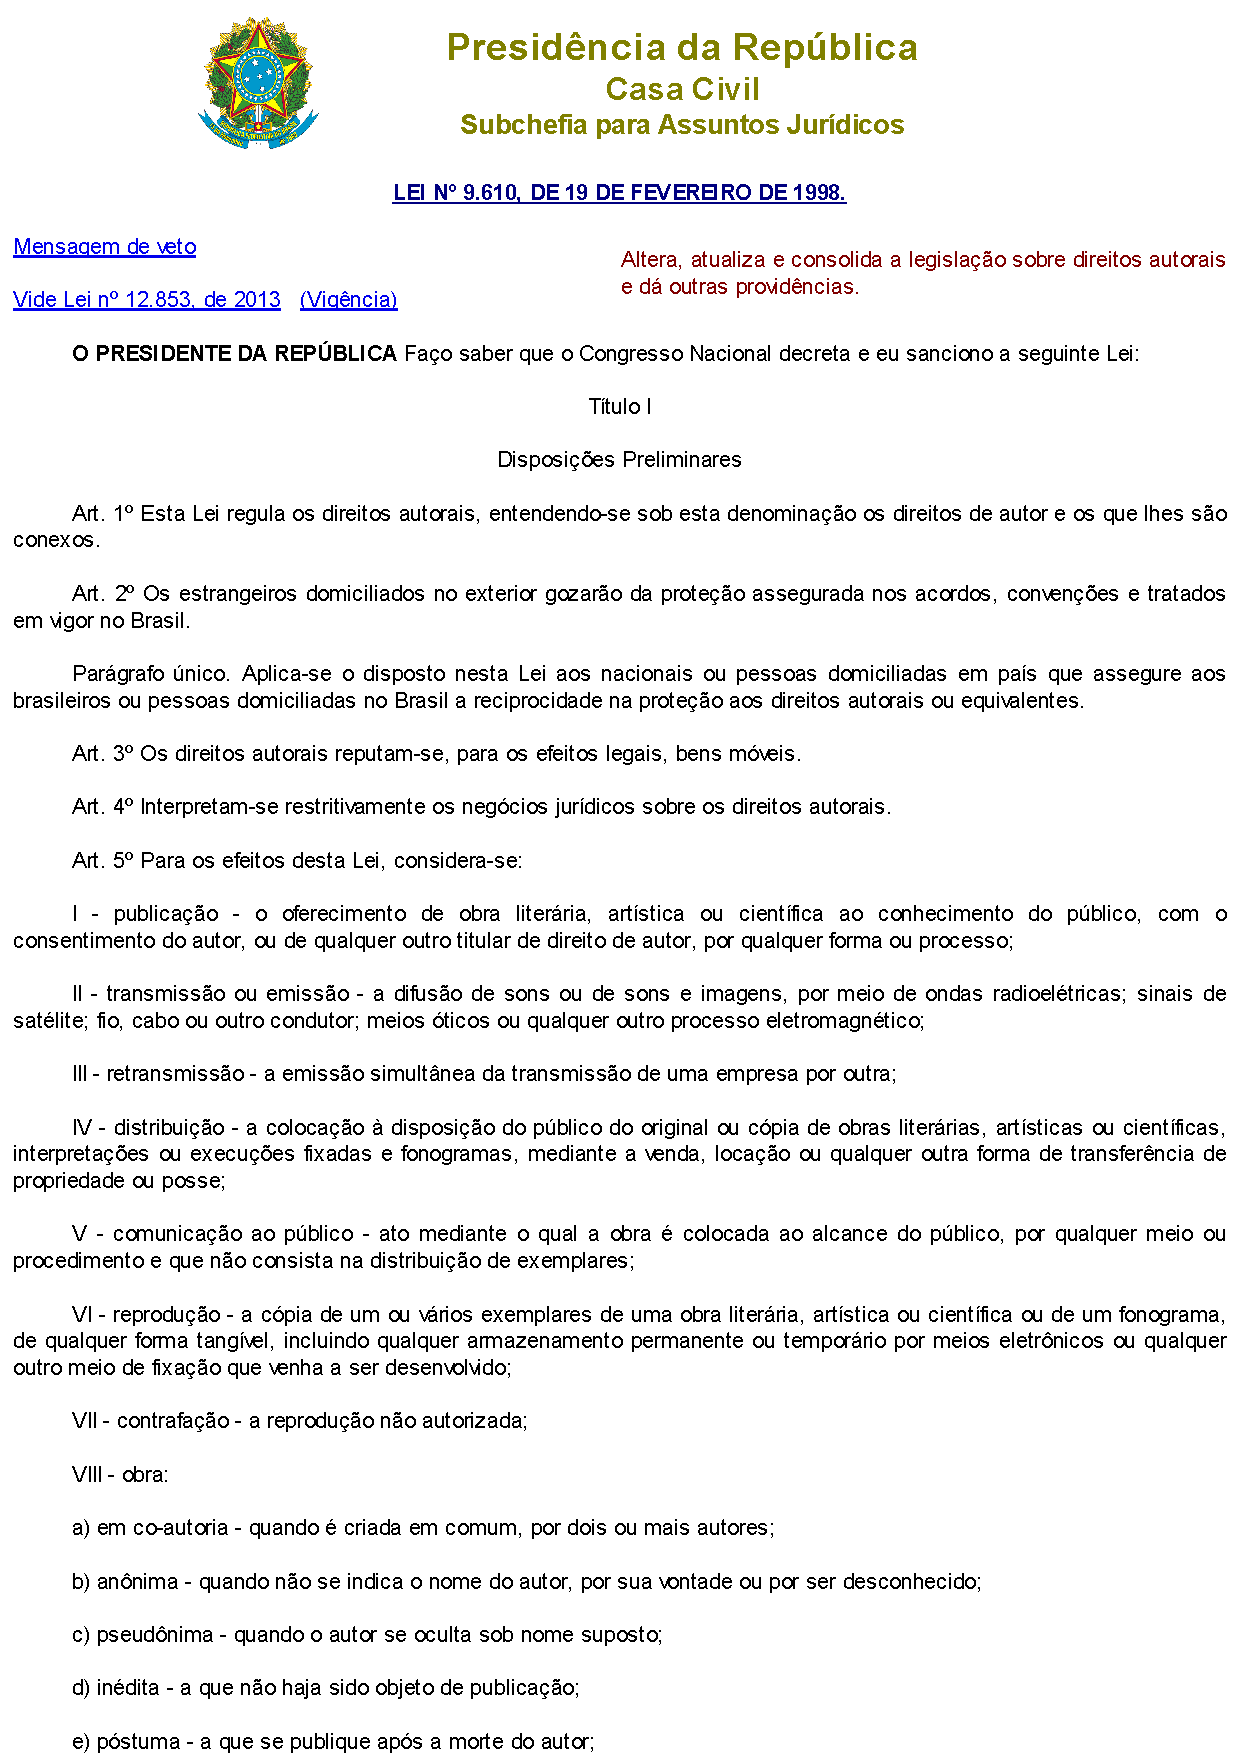
\includegraphics[width=\textwidth]{./PosTexto/Ilustracoes/lei-n9610-p1}}%% Imagem (Dimens\~oes e localiza\c{c}\~ao)

\centerline{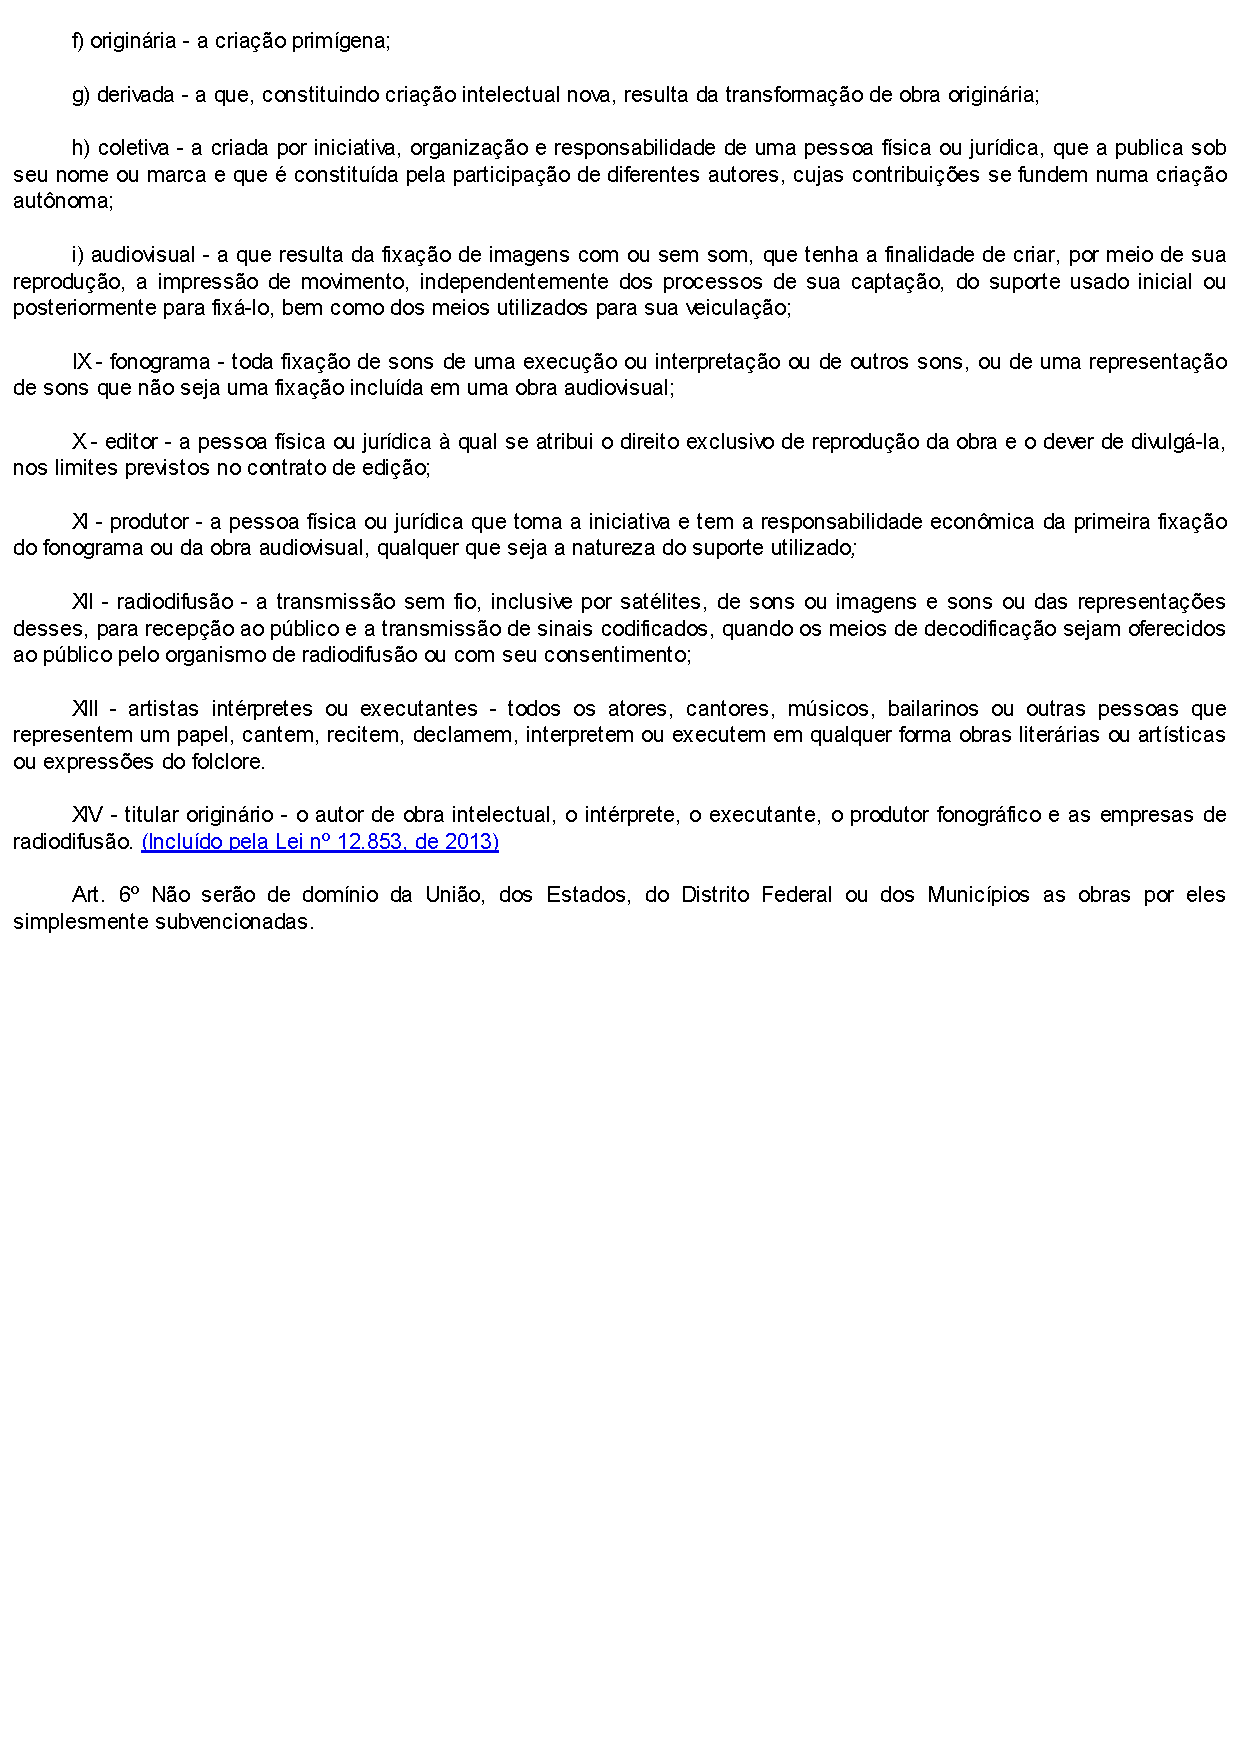
\includegraphics[width=\textwidth]{./PosTexto/Ilustracoes/lei-n9610-p2}}%% Imagem (Dimens\~oes e localiza\c{c}\~ao)
%% Anexo - Comente para remover este item
%  %\include{./PosTexto/anexob}%% Anexo - Comente para remover este item
\end{arquivosdeanexos}%% Não comente esta linha
%%%%%%%%%%%%%%%%%%%%%%%%%%%%%%%%%%%%%%%%%%%%%%%


%%%%%%%%%%%%%%%%%%%%%%%%%%%%%%%%%%%%%%%%%%%%%%%
%% Índice
%%
\incluirindice%% Comente para remover este item
%%%%%%%%%%%%%%%%%%%%%%%%%%%%%%%%%%%%%%%%%%%%%%%

%% Fim do documento
\end{document}%% Não comente esta linha
%%%%%%%%%%%%%%%%%%%%%%%%%%%%%%%%%%%%%%%%%%%%%%%
